\RequirePackage{color}
\documentclass[12pt,frontmatter,copyright,dissertation]{usfmanus}
\usepackage[bottom=1in, left=1in, right=1in, top=1in]{geometry}
\usepackage[utf8]{inputenc}

\usepackage{ifpdf}
\ifpdf %This ensure proper paper size (some compiler like overleaf mess it up)
  \pdfpageheight=11in
  \pdfpagewidth=8.5in
\else
  \special{papersize=11in,8.5in}
\fi

% Block comments
\usepackage{verbatim}

\usepackage[titles]{tocloft}

\newcommand{\subfigureautorefname}{Figure}

% Indent the section levels properly
\setlength{\cftsecindent}{0.5in}
\setlength{\cftsubsecindent}{1in}
\setlength{\cftsubsubsecindent}{1.5in}


\usepackage{multirow}
\usepackage{url} \urlstyle{same} %To keep same font for url
\usepackage{graphicx}
\usepackage{adjustbox}
\usepackage{floatrow}
\usepackage{amsthm}
\usepackage{amsmath}
\usepackage{amssymb,alltt,url,verbatim}
\usepackage{float}
\usepackage{graphics}
\usepackage{graphicx,leftidx}
\usepackage{epsfig}
\usepackage{appendix}
\usepackage[ruled,chapter]{algorithm}
\usepackage{algorithmic}
\usepackage[english]{babel}
\usepackage{url}
\usepackage{multirow}
\usepackage{enumitem}
\usepackage{tabularx}
\usepackage{comment}
\usepackage{amsmath,amssymb,amsfonts}
\usepackage{algorithmic}
\usepackage{textcomp}
\usepackage{xcolor}
\usepackage{multirow}
\usepackage[center]{caption}
\usepackage{subcaption}
\usepackage{balance}
\usepackage{array}
\usepackage{graphicx}
\usepackage{color,colortbl}
\usepackage{booktabs}
%\usepackage{unicode-math}
\usepackage{algorithmic}
\usepackage{graphicx}
\usepackage{textcomp}
\usepackage{xcolor}
\usepackage{comment}
\usepackage{booktabs}
\usepackage{hhline}
\usepackage{pgf}
\usepackage{multirow}
\usepackage{graphicx}
\usepackage{tikz}
%\usepackage{cite}
\usepackage{algorithmic}
\usepackage{textcomp}
\usepackage{xcolor}
\usepackage{multirow}
\usepackage{balance}
\usepackage{array}
\usepackage{pdflscape}
\usepackage{float}
\usepackage{pgfplotstable}
\usepackage{sfmath}
\usepackage{lipsum}
\usepackage{graphicx}
\usepackage{color, colortbl}
\usepackage{graphicx}
\usepackage{tikz}
\usepackage{collcell}
\usepackage{etoolbox}
%\usepackage[table]{xcolor}
\usepackage{booktabs}
\usepackage{hhline}
\usepackage{pgf}
\usepackage{multirow}
\usepackage{graphicx}
\usepackage{tikz}
\usepackage{xcolor}
\usepackage{everypage}
\usepackage{blindtext}
\usepackage{fancyhdr}

\usepackage{tabularx,booktabs}
\usepackage{adjustbox}

%%%for SIMPOR 
\usepackage{mathtools}
\usepackage{cuted}
%%for table 
\usepackage{rotating}
\usepackage{multirow}
\usepackage{booktabs}



%%% for Federated Learning
%%%%%% for privacy section
\usepackage{stmaryrd}



%%%% Only Edit if you know what you are doing %%%
\floatsetup[table]{capposition=top}
\counterwithout{footnote}{chapter}

 \newcolumntype{P}[1]{>{\centering\arraybackslash}p{#1}}

%\captionsetup{justification=raggedright,singlelinecheck=false}
\setlength{\cftbeforetoctitleskip}{-3em}

% correct bad hyphenation here
\hyphenation{op-tical net-works semi-conduc-tor}
\pgfplotsset{compat=1.16}
\newcommand{\Lpagenumber}{\ifdim\textwidth=\linewidth\else\bgroup
  \dimendef\margin=0 
  \ifodd\value{page}\margin=\oddsidemargin
  \else\margin=\evensidemargin
  \fi
  \raisebox{\dimexpr -\topmargin-\headheight-\headsep}[0pt][0pt]{%
    \rlap{\hspace{\dimexpr \margin+\textheight+\footskip}%
    \llap{\rotatebox{90}{\thepage}}}}%
\egroup\fi}
\AddEverypageHook{\Lpagenumber}%


\def\vita{\long\def\@vita}
\def\printvita{%
  \newpage
  \pagestyle{empty}

  \addtocontents{toc}{\protect\contentsline{chapter}%
{About the Author}{End Page}}
  \begin{center}
  ~\\~\\~\\{\bf About the Author} 
  \end{center}
  \begin{doublespace}
   \@vita\nopagebreak\par
  \end{doublespace}
  \vfill
}


%%%%%%%%%%%%%%%%%%%%%%%%%%%%%%%%%%%%

%%%%%%%%%%% Edit from here %%%%%%%%%%%%%%%%%


\title{
		Deep Learning Classification Enhancement and Privacy-Preserving Deep Learning: A Data-Centric Approach
}




\author{Hung S. Nguyen}


\degree{Doctor of Philosophy} 

\distname{dissertation }

\department{Electrical Engineering} 


\college{Engineering} 

\majorprofessor{Morris J. Chang, Ph.D.}

\members{Ismail Uysal, Ph.D. \and
		 Zhuo Lu,  Ph.D. \and
          Lu Lu, Ph.D. \and
          Simon Ou, Ph.D. }
\presentdate{May 29, 2023 (TBD)}

\keywords{Dimentional reduction, Non-IID data, Privacy preservation, Federated learning}

\copyrightyear{2023}

\dedication{\par This dissertation is dedicated to my dear family, including my parents, my sister, and her husband. They initiated my Ph.D. journey by encouraging me to go study abroad. They have supported me a lot throughout my entire studying life. Without their endless mental and economic support, I could not have reached this step. 
	
I am also dedicating this to my beloved wife and in-law family members, including my parents-in-law, sisters-in-law, and brothers-in-law. They all mentally supported me a lot and kept encouraging me to overcome difficulties. My wife especially had to give up her dream job to come and help me through my Ph.D. journey. Without their support, this work was not  possible to complete. }


\acknowledgments{\par First, I would like to express my sincerest gratitude to my advisor,
Professor J. Morris Chang, for his priceless guidance through my Ph.D. journey over
the last five years. I want to thank Prof. Chang for unconditionally supporting me
with academic knowledge, research instructions, and professional career advice, particularly
guiding me to choose research topics that are among the most interesting in the industry
and academia.

I would also like to sincerely thank the professors on my dissertation committee, Dr. Ismail Uysal, Dr. Xinming Ou, Dr. Lu Lu, and Dr. Zhuo Lu. The knowledge that I
have gained from them during coursework and discussions helped enrich this dissertation.

Last but not least, I would like to express my deep gratitude to my academic friends who have been working around me over the past five years. This dissertation would not have been possible without their help.}

\abstract{\par  

Deep Learning and its applications have become attractive to a lot of research recently because of its capability to capture important information from large amounts of data. While most of the work focuses on finding the best model parameters, improving the data still needs more attention. In this work, we propose data processing approaches to enhance the robustness of deep learning classification by improving data quality. Specifically, our data processing proposals aim to alleviate the impacts of class-imbalanced data and non-IID data in classification and federated learning scenarios receptively. In addition, data pre-processing strategies such that dimensionality reduction is also enhanced using deep learning-based techniques for a scenario of data privacy preservation. By conducting several experiments and comparisons, we show that our approaches yield good performance and constantly outperform many state-of-the-art methods.  }


%\vita{\par About the Author}

\setlength{\textfloatsep}{2cm}
\setlength{\intextsep}{2cm}

\begin{document}
	



\chapter{Introduction}
\label{chap:Intro}

In recent decades, deep learning has become successful in many automatic tasks such as pattern recognition, natural language processing, image and vision computing by extracting and learning from large amounts of data. While most existing works focus on enhancing machine learning models to improve task performance, data quality improvement is still in lacks of attention. There are numerous aspects to look for in order to improve data quality, such as data augmentation, data dimensionality reduction, data imbalance, missing data, and feature extraction. In practice, by improving data quality, we could significantly boost machine learning performance. In this work, we aim to enhance machine learning performance by focusing on data processing techniques to alleviate the negative impacts of class imbalance, data that is not independent and identically distributed (non-IID). Besides, we also propose a deep learning-based dimensionality reduction technique to improve classification accuracy and preserve user privacy simultaneously. Proposed techniques are introduced in the following chapters. Specifically, Chapter \ref{chap:FedDisk} introduces a method to tackle the non-IID issue in federated learning, which might significantly reduce machine learning performance. Chapter \ref{chap:SIMPOR} introduces a class balancing technique that generates synthetic data for minor classes. This could help deep learning to avoid slow convergence problems and task performance. In Chapter \ref{chap:AUTOGAN}, we propose a dimensionality reduction technique based on the state-of-the-art generative models (i.e., AutoEncoder and Generative Adversarial Network) to not only improve classification accuracy but also preserve data privacy. 



\newcommand{\MethodnameLong}{Federated Learning for Skewed Distribution Using Sample Weights}
\newcommand{\MethodnameShort}{FedDisk}

\newcommand{\px}[2]{p_{#1}(\mathbf{x_{#2}})}
\newcommand{\qx}[2]{q_{#1}(\mathbf{x_{#2}})}

\newcommand{\Prob}{\mathcal{P} }


\newcommand{\x}{\mathbf{x}}
\newcommand{\ubold}{\mathbf{u}}

\newcommand\parties{100}



%for figure paths
\newcommand{\ChapterPathFedDisk}{Chapter2} 


\chapter{Federated Learning for Skewed Distribution}
\label{chap:FedDisk}




\section{Introduction}
\label{sec:FedIntro}
Since the demand for massive data in artificial intelligent machines, the concept of federated learning (FL) was first introduced in 2017 \cite{OriginFL}, which is a collaboratively decentralized learning framework. In contrast to centralized learning approaches (in which datasets are sent to an aggregator), FL encourages data holders to contribute without the privacy concern of exposing their raw data. For example, several hospitals holding patient records would participate in a machine learning system to provide better disease predictions via a FL framework without the concern of privacy disclosure. Since then, FL has been seen in various applications in different fields \cite{abs-1811-03604,yadav_federated_2022,feki_federated_2021,zhai_dynamic_2021}. 

To learn a model utilizing data from multiple clients without directly accessing to clients' data, authors in \cite{OriginFL} introduced Federated Averaging (FedAvg) and demonstrated its robustness. The main idea is that clients (data holders) involve in a model training process by exchanging local models' weights instead of exchanging raw data. One of the main concerns in FL is that the data might come from different sources and have different distributions. Thus, FL performance is significantly reduced because this violates a fundamental machine learning assumption that data should be independent and identically distributed (IID). The FL over non-IID data has been shown in existing works \cite{ZHU2021371,Sahu2018OnTC,9392310,abs_1905_06641,Shen2020FederatedML,9155494,abs-2102-02079,abs-2005-11418} that its performance deteriorates dramatically. In this work, we focus on tackling the non-IID data issue in a federated learning system, in which the collected data feature distribution is skewed. The skewness might be caused by many different reasons. For example, clients might perform different sampling methods, apply different normalization methods, or sample using different devices. 

Over the past few years, there have been a number of approaches aiming at reducing non-IID data impacts. While many current works focus on the skewed label distribution, there are only limited approaches considering skewed feature distribution data which is very common in various fields, e.g., medical images collected from different x-ray machines. Authors in \cite{Zhao2018FederatedLW} explained the performance reduction as the problem of weight divergence. They then proposed an alleviation by combining local data with global shared data to train each client. However, it raises the concern of privacy violation with the shared data. Li et al. illustrated in their work (FedBN) \cite{li2021fedbn} that Local Batch Normalization would help to reduce the problem of non-IID data. FedBN suggests clients to not synchronize local batch normalization parameters with the global model. Sahu et al. introduce FedProx \cite{FedProx} to solve the weight-divergence issue by proposing a loss function which constrains the local models to stay close to the global model. FedDNA \cite{fedDNA} shares statistical parameters of models (means and variances) and aims at finding averaging weights for each client's model to minimize models' weights divergence across clients. However, as this only considers the aggregating weights for each model, the improvement is minor. FedNova \cite{fednova} suggests to normalize local weights before synchronizing with the aggregator. FedMA \cite{fedma}, AFL \cite{AFL} and PFNM \cite{pfnm} consider combinations of layer-wise parameters and provide an aggregation of such parameters to alleviate the non-IID issue. In FedRod \cite{FedRod}, Chen and Chao deal with the non-IID issue by learning hyper-networks locally which results in personalized classifiers for clients and clients' class distributions. Recently, Tan et al. \cite{FedProto} tackle the non-IID data issue by exchanging representation vectors of samples in a given class instead of model's parameters, enable clients to have personalized model architecture. However, these suggestions do not directly consider the data distribution skewness at the data level, which could lead to performance reduction and convergence slowth.    

Different from centralized learning frameworks, the non-IID issue is challenging in FL because of the limited access to client's raw data. To overcome this, we propose an algorithm that implicitly leverages statistical information of client data to alleviate the distribution skewness impact. Our method only requires clients to exchange additional model weights using a typical FL procedure. The proposed method aims to exchange statistical information to generate sample weights to adjust distribution skewness at the sample level. After acquiring the adjusting weights, the machine learning model can be trained under a typical FL framework. Similar to a typical FL framework, the proposed method does not require clients to expose their private data.
Our contributions are as follows:
\begin{enumerate}
	\item Provide a theoretical base to deal with skewed feature distribution data for federated learning by adjusting sample weights derived from the machine learning empirical risk.  
	\item Provide a practical solution to mitigate the problem of learning from non-IID data for the FL framework without sharing clients' draw data. It not only helps to improve the classification accuracy of the global model but also accelerates the model convergence process, thus minimizing communication costs.
	\item Several experiments were conducted on three datasets, including MNIST, non-IID benchmark dataset FEMNIST and real-world dataset Chest-Xray. The results demonstrate that the proposed method outperforms other experimental methods in classification accuracy and dramatically reduces the communication cost.
	\item As the proposed method needs to exchange additional information, we also provide a theoretical analysis to analyze the potential privacy leakage. We showed that the leakage information becomes insignificant when the number of clients increases. 
	\item To our best knowledge, the proposed method is the first method utilizing data distribution information and sample weights to tackle the FL Non-IID issue.   
\end{enumerate}

The rest of this paper is organized as follows. Section \ref{sec:FedProblem} introduces our problem in a scenario where clients hold different distribution datasets. Section \ref{sec:made} introduces a neural network-based model is leveraged in our work to carry density information. Our proposed solution is introduced in Section \ref{sec:FedMethodology}. We provide a privacy leakage analysis in Section \ref{sec:FedPrivacyAnalysis} as the proposed method indirectly exchanges distribution information. Section \ref{sec:FedExperiments} shows our experimental results and illustrates the proposed method's performance. Section \ref{sec:FedConclusion} summarizes our study and discusses the future work to improve the proposed method.        

\section{Preliminary: Masked Autoencoder for Distribution Estimation}
\label{sec:made}
The proposed method asks the clients to share additional model weights that carry their local datasets' distribution information instead of sharing the raw data. We utilize a neural network-based density estimation, namely, Masked Autoencoder for Distribution Estimation (MADE) \cite{MADE}. This section briefly introduces MADE.

MADE is designed to estimate the probability distribution of input components (e.g., pixels in an image). MADE assumes input components are dependent instead of independent, which is relevant in many applications. For example, MADE can decompose the distribution of an instance $\textbf{x}$ consisting d components $x_1, x_2, x_3, ..., x_n$ as follows:

\begin{equation}
\label{eq:MADE_decomposition}
p(\mathbf{x}) =   p(x_1|x_2,x_3,..,x_n) \cdot p(x_2|x_3,...,x_n) 
...p(x_{n-1}|x_n) \cdot p(x_n). 
\end{equation}

For implementation, MADE poses the constraint on a neural network model that each output component in a certain layer only connects to its dependent input components in the previous layer. Masks are created based on such principle, and applied to the weights of the model.
Specifically, MADE assigns each unit in a hidden layer an integer $\textit{m}$ between $1$ and $D-1$, where $D$ is the number of dimensions. Denote $\textit{m(k) } $ as the maximum number of units in the previous layer to which the $\textit{k}^{th}$ hidden unit can connect, the weight mask $M$ is then formulated as follows:

\begin{equation}
 M_{k,d} = 1_{m(k) \geq d} = 
				 \begin{cases}
				  1 & \text{if \textit{m(k)} $\geq$ d }\\
				  0 & \text{otherwise,}
				 \end{cases} 
\end{equation}
for $d \in \{1,...,D\}$ and $k \in \{1,...,K \}$ with $K$ being the number of hidden layer units.


\section{Scenario}
\label{sec:FedProblem}
In this section, we introduce and formulate the scenario of FL with skewed feature distribution across clients. 
Our scenario is a learning collaboration between $K$ clients to build a global classification model that maximizes the global accuracy given arbitrary data. Each client holds a number of individual records that they are not willing to share with others due to privacy concerns. This study focus on preventing the performance of the global model from deteriorating because of the distribution skewness issue \cite{survey} across clients.

We denote the data and associated labels held by client $k$ $\in$ $\{1,...,K\}$ as $ \{( \mathbf{x}_k^i,y_k^i )\}_{i=1}^{N_k}$ where $ \mathbf{x}_k^i \in \mathbb{R}^d$ and $y_k^i \in \mathbb{N}$. Instead of learning each model for every client $f(\mathbf{w}_k)$ (where $f(\cdot)$ demotes local inference models and $\mathbf{w}_k$ is the model's parameter of the $k^{th}$ client), the objective is to maximize the performance of a global model $g(\mathbf{w})$ ($g(\cdot)$ approximates the global inference model and $\mathbf{w}$ is the global model's parameter) that is resilient to data skewness.  

\section{\MethodnameLong{}}
\label{sec:FedMethodology}
\label{sec:methodology}
In this section, we propose a solution to alleviate the negative impact of distribution skewness across clients for federated learning. The proposed method aims to find weights for training samples in order to adjust the global distribution. To achieve this goal, we need to exchange some statistical information between clients and the aggregator in a privacy-preserving manner. The remainder of this section introduces how we design sample weights, how we exchange statistical information without exposing clients' raw data, and how we derive sample weights from achieved information. After achieving weights for the samples, the training process for machine learning tasks is similar to FedAvg \cite{OriginFL}. Our framework is illustrated in Figure \ref{fig:framework}. The proposed method, namely \MethodnameShort{}, requires a 2-phase process. First, clients jointly learn a global density estimation model and their local density models utilizing MADE models. These models are then used to derive sample weights for the local training process. Second, the machine learning tasks can be learned by the conventional FL procedure, with the data skewness issue mitigated by the sample weights from the first phase.
\begin{figure*}[ht!]
	\centering
	%left bottom right top,
	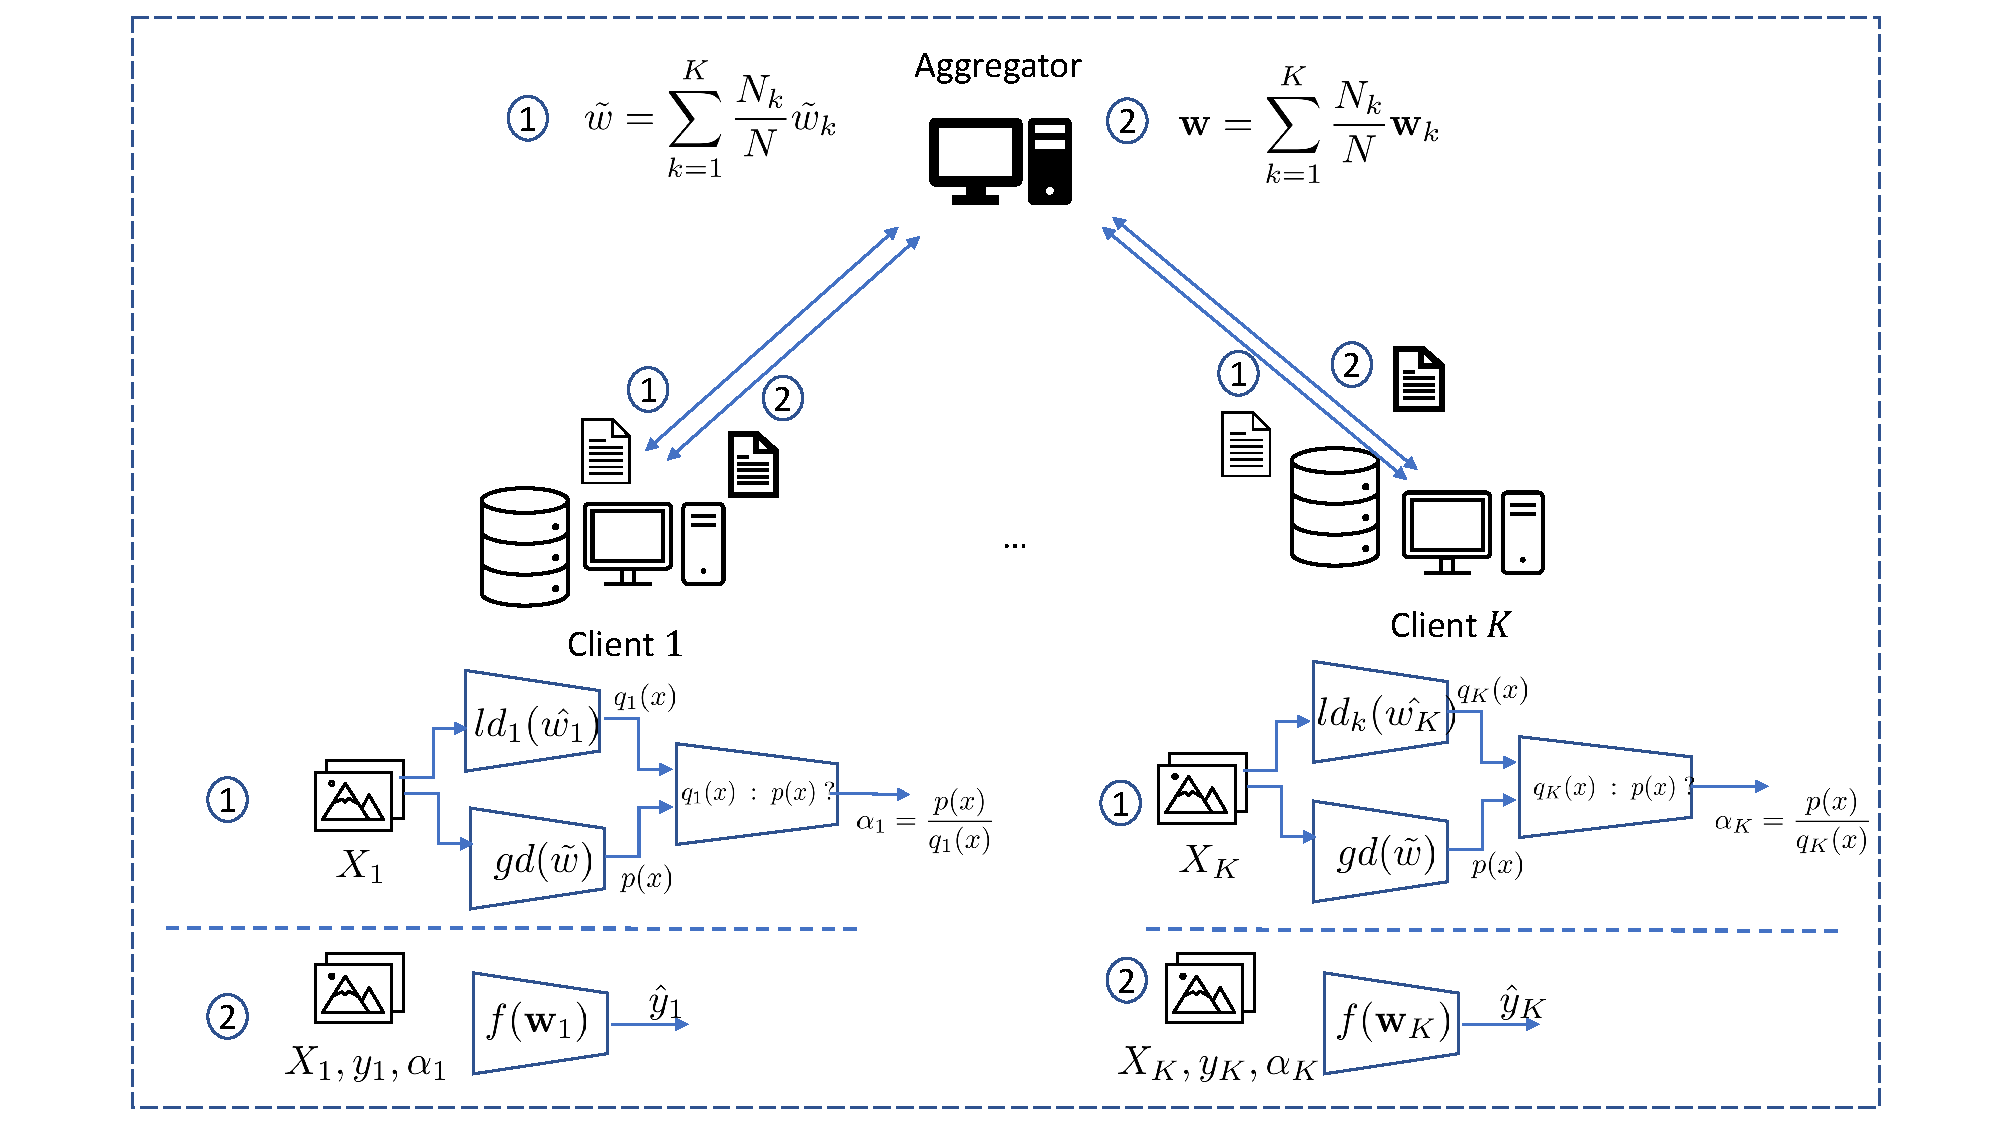
\includegraphics[width=0.85\textwidth, trim={1cm 0.1cm 1cm 0.3cm},clip]{\ChapterPathFedDisk/Figures/FL}
	\caption[\MethodnameShort{} framework.]{\MethodnameShort{} framework. The proposed framework has two phases. First, local and global probability density functions ($p(x),q(x)$) are estimated via MADE models leveraging FL procedures. Then, the sample weights $\alpha$ are computed by approximating density ratio via class probability estimation. Second, the machine learning tasks (e.g., classification) can be performed similar to a typical FL method (i.e., FedAvg) with the sample weights acquired from phase 1.} 
	\label{fig:framework} 
	
\end{figure*}  

\subsection{Sample Weights Design}
As we do not have sufficient information about the true distribution, we consider the combination of all clients' dataset distribution as our true distribution. Thus, we consider the probability density function (pdf) of the true distribution as 

\begin{equation}
\label{eq:sumdist}
p(\mathbf{x}) = \sum_{k=1}^{K}q_k(\mathbf{x}) ,
\end{equation}
where $q_k(\mathbf{x})$ represents the pdf of the $k^{th}$ client's data. 

To jointly learn a global model, the system finds the expectation of the loss function $l(g(\mathbf{x}),y)$ with sample $\x{}$ that drawn from the true distribution. The expected loss is formulated by the associated risk \cite{noauthor_empirical_2021} as follows:

\begin{align}
\mathbb{E}[l(g(\mathbf{x}),y)] 
% &= \iint l(g(\mathbf{\mathbf{x}}),y) p(\mathbf{x},y) d\mathbf{x}dy \label{eq:risk1}\\
&= \iint l(g(\mathbf{x}),y) p(y|\mathbf{\mathbf{x}}) p(\mathbf{x}) d\mathbf{x}dy, \label{eq:risk} 
\end{align}
where $p(\mathbf{x},y)$ is the joint pdf of a sample $\mathbf{x}$ and its associated label $y$, and $p(y|\mathbf{x})$ is the conditional probability of a label $y$ given a sample $\mathbf{x}$. We also assume that for any client $k \in$ $\{1,...,K\}$ with local data distribution $q_k(\mathbf{x})$, the conditional probability of a label $y$ given a sample $\mathbf{x}$ is equivalent to that of the true distribution, namely

\begin{align}
\label{eq:assumtion}
q_k(y|\mathbf{x}) = p(y|\mathbf{x}).
\end{align}

From Equation \ref{eq:sumdist}, \ref{eq:risk}, \ref{eq:assumtion}, and by multiplying with factor $\frac{q_k(\mathbf{x})}{q_k(\mathbf{x})}=1$, the expected loss in Equation \ref{eq:risk} can be expanded as follows:

\begin{align}
\mathbb{E}[l(g(\mathbf{x}),y)]  &= \iint l(g(\mathbf{x}),y) p(y|\mathbf{x}) p(x) d\mathbf{x}dy,\\
%&= \iint l(g(\mathbf{x}),y) p(y|\mathbf{x}) \frac{q_k(\mathbf{x})}{q_k(\mathbf{x})}  p(\mathbf{x}) d\mathbf{x}dy	 \\
&= \iint l(g(\mathbf{x}),y) q_k(y|\mathbf{x}) \frac{q_k(\mathbf{x})}{q_k(\mathbf{x})}  p(\mathbf{x}) d\mathbf{x}dy \\
&= \iint l(g(\mathbf{x}),y) q_k(\mathbf{x},y) \frac{p(\mathbf{x})}{q_k(\mathbf{x})}  d\mathbf{x}dy.    \label{eq:expectedloss}
\end{align}

The objective of the global model thus amounts to minimize the empirical risk over all $K$ clients' datasets:

\begin{equation}
\begin{aligned}
\underset{g}{\text{minimize}}
\sum_{k=1}^{K} \frac{1}{N_k}\sum_{j=1}^{N_k} \alpha_k^j \:l(g(\mathbf{x}_k^j),y_k^j)), \label{eq:optimation}
\end{aligned}
\end{equation} 
where $\mathbf{x}_k^j$, $y_k^j$ are the $j^{th}$ sample and its label. $N_k$ is the number of samples in the $k^{th}$ client's dataset. $\alpha_k^j$ is the corresponding sample weight computed as

\begin{equation}
\begin{aligned}
\boxed{\alpha_k^j = \frac{ \px{}{}}{q_k(\mathbf{x})}  = \frac{ \sum_{i=1}^{K}q_i(\mathbf{x}) }{q_k(\mathbf{x})}. }  
\label{eq:alpha}.
\end{aligned}
\end{equation}

Our problem becomes minimizing the summation of the loss functions (Equation \ref{eq:optimation}) over all clients. For each client, the loss function is minimized over local samples with the corresponding $j^{th}$ sample weight of the client $k^{th}$, $\alpha_k^j$. The sample weights could be estimated by the density ratio between the true distribution (global distribution) and the client distributions (local distributions). For each client, the local distribution can be estimated using its local data. However, the challenge is to achieve the true distribution without having access to other clients' data. To solve this, we leverage a neural network-based density estimation model to learn the global density function via a typical federated learning procedure. Thus, clients can implicitly exchange some statistical information, while still preserving the privacy in client data.          


\subsection{Probability Density Approximation}
\label{sec:densityapproximation}
To estimate global density and preserve client privacy at the same time, we propose to leverage a neural network-based density estimation so that we can exchange local density information (via models' weights) with the aggregator without sharing the raw data. In this work, we leverage a well-known method, namely, Masked Autoencoder for Distribution Estimation (MADE, \cite{MADE}), which is briefly reviewed in Section \ref{sec:made}. Elaborately, each client aims to estimate its local probability density $q_k(\mathbf{x})$ using its own dataset, and all $K$ clients jointly estimate the global probability density $p(\mathbf{x}) = q_1(\mathbf{x})+...+q_K(\mathbf{x})$. Learned MADE models are used to approximate local probability density functions, and the global MADE model approximates the global probability density. The learning process is described as follows.    

The $k^{th}$ client learns a local density estimation model $ld_k(\hat{w}_k)$ (where $ld(\cdot)$ approximates density estimation function with parameter $\hat{w}$) using its local data. It then jointly learns a global density estimation model $gd(\tilde{w})$ (where $gd(\cdot)$ represents the global density function with the parameter $\tilde{w}$) using the procedure similarly to FedAvg \cite{OriginFL}. Specifically, for the local model density estimation models, each client train a MADE model on its local data until the loss function can not be improved. For the global density estimation model, each client trains its data locally for a certain number of iterations, and then model parameters are sent to an aggregator for the aggregation. Since clients might own different number of samples, a weight of ${N_k}/N$ (where $N_k$ and $N$ are the number of samples of the $k^{th}$ client and the the total number of samples over all clients) is used for adjusting client parameter significance, similar to FedAvg. After aggregating all clients' model parameters, the aggregator shares global model parameters to all clients. The steps are repeated until the validation loss starts increasing. The global MADE model aggregation from $K$ clients at iteration $t$ can be described as follows:

\begin{equation}
\begin{aligned}
\tilde{w}^t = \frac{N_k}{N}\sum_{k=1}^{K} \tilde{w}^t_k 
\end{aligned}
\end{equation}

\subsection{Sample Weight Approximation}
\label{sec:weightapproximation}
After the local and global density approximations by MADE models are fully learned ( Section \ref{sec:densityapproximation}), we can estimate sample weights in Equation \ref{eq:alpha}. Since MADE models output vectors of conditional probabilities for each element in the d-dimensional input $\mathbf{x}$, an intuitive way to compute $p(\mathbf{x})$ is to multiply all the conditional probabilities. However, as $\px{}{}$ vanishes when any of the conditional probabilities vanishes, we instead keep the output as a vector of conditional probabilities (same size as input) and approximate the density ratio in Equation \ref{eq:alpha} using a class probability estimation method inspired by \cite{densityratio}. The method aims at training a binary classifier to output a probability that represents the ratio between $\px{}{}$ and $\qx{}{}$. The solution detail is described in the rest of this subsection. 

After each client receives the final global MADE model and trains its own local MADE, it starts to evaluate sample weights for its local data. The training data of the $k^{th}$ client, $X_k$, is then fed into both the global MADE (the global MADE is downloaded to clients so that this step can be done locally) and the local MADE to estimate $\px{}{}$ and $\qx{k}{}$, respectively. Denote $\ubold{}$ as the output vector of density estimation models, and $l$ be the pseudo label indicating whether it is sampled from the global destination ($l=1$) or the local distribution ($l=0$). Each client then trains a binary classifier to differentiate whether the output $\ubold$ comes from $\px{}{}$ or $\qx{k}{}$. Outputs of the two MADE models (the sample size of each output is $N_k$) are concatenated to a new vector dataset including samples $\{(\ubold{}_k^i,l_k^i) \}_{i=1}^{2N_k}$, and is used to train the binary classifier. The conditional probabilities of the binary classification model $h(\ubold,w_h)$ (where $\ubold$ is the input variable , $w_h$ is the model parameter) can be approximated as following: 

\begin{align}
\Prob(\ubold | l=0 )  \propto  \qx{k}{}  ,\;\;\;\;
\Prob(\ubold | l=1 )  \propto \px{}{}.
\end{align}

From Bayes' rule, we have

\begin{align}
\frac{\px{}{}}{\qx{}{}} &= \frac{\Prob(\ubold | l=1 )}{ \Prob(\ubold | l=0 ) }       
= \left( \frac{\Prob(l=1| \ubold ) \Prob(\ubold)}{\Prob(l=1)} \right)     
\left( \frac{\Prob(l=0)} {\Prob(l=0| \ubold ) \Prob(\ubold)}\right)  \label{eq:pq1}\\
&= \frac{  \Prob(l=1|\ubold )  \Prob(l=0) }{ \Prob(l=0|\ubold )  \Prob(l=1)  }.  \label{eq:pq2} 
\end{align}

We approximate the marginal probability ratio between two distributions ( $\Prob(l=0)$  and $\Prob(l=1)$) by the number of samples from the two distributions $N_k$ over the concatenated dataset size ($2N_k$).Thus,  We have
$\frac{ \Prob(l=0) }{ \Prob(l=1)  } = \frac{N_k}{2N_k} \frac{2N_k}{N_k}=1. \label{eq:marginalratio}$


The density ratio then can be estimated as follows:
\begin{align}
\frac{\px{}{}}{\qx{}{}} &= \frac{  \Prob(l=1|\ubold )  }{ \Prob(l=0|\ubold )   } 
= \frac{  \Prob(l=1|\ubold )  }{ 1 - \Prob(l=1|\ubold )   }. \label{eq:ratio2}
\end{align} 
where $\Prob(l=1|\ubold{})$ is the classifier's probability-liked output indicating how likely an input vector $\ubold$ comes from the global probability $\px{}{}$. 

To summarize, the $j^{th}$ training sample of client $k$, $\x_k^j$, is fed into the client's local MADE model to achieve its corresponding density estimation $\ubold{}_k^j$. $\ubold{}_k^j$ is then fed into the binary classification function $h(\ubold)$ to achieve the class probability $ \Prob(l=1|\ubold_k^j ) $. This is used to estimate the sample weight $\alpha_k^j$ (Equation \ref{eq:alpha}) based on Equation \ref{eq:ratio2}. In words, the binary classification model $h(\ubold,w_h)$ is expected to return higher weights for samples that are likely belonging to the true distribution and vice versa. 

\subsection{Learning on Skewed Distribution Data Across Clients }
After acquiring sample weights, each client starts to train the model on the local dataset and corresponding sample weights for a machine learning task (e.g., classification) as a typical FL framework. In this work, we follow the procedure introduced by FedAvg to learn the global model. The aggregator aggregates clients' local models as follows:

\begin{equation}
\begin{aligned}
\mathbf{w}^t = \frac{N_k}{N}\sum_{k=1}^{K} \mathbf{w}^t_k 
\end{aligned}
\end{equation}
where $\mathbf{w}^t$ and $\mathbf{w}^t_k$ are the global and local model parameter of $k^{th}$ client at the $t^{th}$ iteration.


\section{Privacy Leakage Analysis}
\label{sec:FedPrivacyAnalysis}
In this section, we discuss the privacy leakage of our method compared to the conventional FL. Similar to many other works, we utilize additional information to alleviate the negative impact of non-IID data, i.e., parameters of MADE models. However, these parameters might contain distribution information of clients’ data. However, we prove that the more clients are involved in the FL training process, the less information is leaked. The detail is described as follows. 

Assume each client samples their own data point ${\hat Z}_k \sim Q_k$ independently, and let  $\Theta$ be a random variable taking values in $\llbracket 1,K \rrbracket$ with $\Prob[\Theta = k] = \kappa_k$ and independent of ${\hat Z}_k$ for each $k \in \llbracket 1,K \rrbracket$. Note that ${\hat Z}_\Theta \sim P$, and one may quantify the privacy leakage of client $k$'s data through the knowledge of $P$ by the mutual  information between ${\hat Z}_k$ and ${\hat Z}_\Theta$, as given by

\begin{equation}
\begin{aligned}
I({\hat Z}_k;{\hat Z}_\Theta) & \leq I({\hat Z}_k;{\hat Z}_\Theta, \Theta)
=  I({\hat Z}_k; \Theta) + I({\hat Z}_k;{\hat Z}_\Theta | \Theta)
\\ &= I({\hat Z}_k;{\hat Z}_\Theta | \Theta) = \sum_{i=1}^K \Prob[\Theta = i] I({\hat Z}_k;{\hat Z}_i) = \kappa_k H({\hat Z}_k).
\end{aligned}
\end{equation}
%
In other words, the privacy leakage is proportional to $\kappa_k$, which decreases to $0$ as long as $\kappa_k = O(1/K)$ and $K \rightarrow \infty$.

\section{Experiments}
\label{sec:FedExperiments}
In this section, we conduct several experiments to evaluate the proposed method on non-IID FL scenarios with three real image datasets (MNIST, Chest-Xray and FEMNIST). Our FL system goal is to learn a global classifier leveraging data from all clients. The classification accuracy is used as a metric to evaluate the performance of the proposed method. The communication cost is evaluated by counting the number of iterations needed for clients to exchange model parameters with the aggregator. We compare our method with other state-of-the-art methods, e.i., FedAvg, FedProx, FedBN, and FedROD. 

\subsection{Datasets and Non-IID Setting.}
In this Section, we describe how datasets are used in our experiments. We categorize our dataset into two groups, simulated non-IID dataset (MNIST) and real non-IID datasets (Femnist \& Chest Xray). The first one contains images that have already been combined together so that our partitioning process is considered for sampling from the same contribution. Thus, we added different levels of noise to each client to simulate the feature skewness as inspired by settings in \cite{abs-2102-02079}, and \cite{FedProto}. The second group's data are collected from different sources so that they are considered to be non-IID by nature. All the data are normalized and clipped to the range of [0,1] before training. Each client's data is split to 85\% and 15\% for training and testing sets, respectively. The detail of the datasets is described as follows.  

\subsubsection{Simulated Non-IID: MNIST}
MNIST dataset \cite{deng2012mnist} contains 60,000 (1x28x28) gray scale images of 10 digits (0-9). The number of unique output labels is 10 representing 10 digits. To mimic feature skewness, we split data equally into \parties{} partitions and add different level of noise to each client's data as inspried by the skewness simulation in \cite{abs-2102-02079}. The noise is drawn from Gaussian distribution with a mean of 0 and different values of standard deviations. More specifically, the $k^{th}$ client $(k \in [0,99])$ is added noise with the variance of $k*x/100$ where $x$ is the added noise variance.  

\subsubsection{Real Non-IID: Femnist and Chest Xray}
FEMNIST dataset is downloaded from https://leaf.cmu.edu/, which is considered a benchmark dataset for real non-IID data. It contains handwritten images of 62 digits and characters (corresponding to 62 unique labels) from different writers and strokes. In this study, we randomly select \parties{} different writers (each of them owns more than 300 images to avoid overfitting) and assign their data to \parties{} clients. The average sample size of clients is 387.47, and the standard deviation is 83.04. All images are resized to a (32x32) grayscale and normalized to the range of [0,1] before inputting to models.

The Chest-Xray dataset, which contains pneumonia and normal chest xray images, are collected from different sources (i.e., COVID-19 \cite{covid19}, Shenzhen Hospital \cite{Shenzhen}, and University of California San Diego (UCSD) \cite{Kermany2018LabeledOC}) with different image sizes, colors and potentially taken from different medical devices. Thus, we consider this dataset non-IID by nature. After partitioning the data into \parties{} clients, the mean and standard deviation of the client sample size are 325.50 and 63.74, respectively. All images are converted to grayscale and resized to (32x32). There are two unique output labels (binary classification) to predict chest xray images are normal or abnormal.

\subsection{Implementation Detail}
\subsubsection{Baselines}
We compare our methods with different methods, i.e., FedAvg, FedProx, FedBN, and FedROD. While most implementation details are taken from the initial parameter sets in original papers, we also tune suggested parameters and report the results that give the best values. For FedROD, the results are reported for the hyper-parameter $\mu$ of 1. We also tried other values in the set {1, 5, 10, 20} and found that the results are very similar. For FedProx, we tuned the parameter $\mu$ with the candidates of {0.001, 0.01, 0.1, 1} and reported the value of 0.01, 1, 0.01 for the three datasets, Chest-Xray, FEMNIST, MNIST, respectively. 

\subsubsection{Federated Learning Classification Model} We use shallow Convolutional Neural Networks (CNN) for the classification of image datasets. The models are constructed by two 5x5 convolutional layers (32 and 32 channels for Chest-Xray, 128 and 128 channels for FEMNIST, 32 and 32 channels for MNIST). Each convolutional layer is followed by 2x2 max pooling and batch normalization layers. A fully connected layer with 16 neurons is added on the top of the models. The input and output sizes are designed to fit each dataset scenario (i.e., image size and the number of unique labels). We use stochastic gradient descent (SGD) with a learning rate of 0.01 for the optimizers. Local iterations are set to 2 for all datasets. Global iterations are set to 1500 for FEMNIST and MNIST, and 500 for Chest-Xray. 

\subsubsection{Density Estimation Model (MADE)} Density estimation models (MADE) are constructed by neural networks and the hyper-parameters are taken directly from the initial setting for MNIST dataset by the original work \cite{MADE}. More detail, the models include a 500-neuron hidden layer. We also tried different settings of MADE. For example, the number of layers was tuned within the set of {1,2,3} and 500 neurons in each layer. However, the three settings gave very similar results. Thus, we select one hidden layer as it is the optimized setting. The model's input and output sizes are the flattened size of images. For example, the input and output size is 784 for MNIST dataset with an image size of 28x28. The maximum iteration is 500, and the training process is stopped when the validation loss starts increasing. Other hyper-parameters are taken directly from \cite{MADE}.

\subsubsection{Sample Weight Approximation} In order to compute the sample weight $alpha$, we use a shallow, fully connected neural network to discriminate the density estimation output vectors coming from which of the two distribution density functions $\px{}{}$ or $\qx{}{}$. The model contains a 100-neuron hidden layer with Relu activation function. The output layer contains one neuron with Sigmoid activation function. All models applied a learning rate of 0.01, and SGD optimization were used in the training process. The training process is terminated if the loss function is not significantly reduced.

\subsection{Results}
\begin{figure*}[ht!]
	\centering
	%[trim=left bottom right top, clip]
	\begin{subfigure}[t]{0.3\linewidth}	
		\includegraphics[width=\linewidth]{\ChapterPathFedDisk/Figures/xray/test_acc}
		\caption{Chest-Xray }
		\label{fig:acc_xray}
	\end{subfigure}
	\hspace{0.01em}%
	\begin{subfigure}[t]{0.3\linewidth}
		\includegraphics[width=\linewidth]{\ChapterPathFedDisk/Figures/femnist/test_acc}
		\caption{FEMNIST}
		\label{fig:acc_femnist}
	\end{subfigure}
	\hspace{0.01em}%
	\begin{subfigure}[t]{0.3\linewidth}	
		\includegraphics[width=\linewidth]{\ChapterPathFedDisk/Figures/mnist/test_acc}
		\caption{MNIST (NoiseVar 0.3)  }
		\label{fig:acc_mnist}
	\end{subfigure}
	\caption[Classification accuracy over global iterations.]{Global model's average test accuracy during aggregation process. For MNIST dataset, clients' data were added noise with the mean of zero and variance of 0.3.}
	\label{fig:acc_all}
\end{figure*}

\begin{figure*}[ht!]
	\centering
	%[trim=left bottom right top, clip]
	\begin{subfigure}[t]{0.3\linewidth}	
		\includegraphics[width=\linewidth]{\ChapterPathFedDisk/Figures/xray/ClientAcc}
		\caption{Chest-Xray }
		\label{fig:cl_acc_xray}
	\end{subfigure}
	\hspace{0.01em}%
	\begin{subfigure}[t]{0.3\linewidth}
		\includegraphics[width=\linewidth]{\ChapterPathFedDisk/Figures/femnist/ClientAcc}
		\caption{FEMNIST}
		\label{fig:cl_acc_femnist}
	\end{subfigure}
	\hspace{0.01em}%
	\begin{subfigure}[t]{0.3\linewidth}	
		\includegraphics[width=\linewidth]{\ChapterPathFedDisk/Figures/mnist/ClientAcc}
		\caption{MNIST (NoiseVar 0.3) }
		\label{fig:cl_acc_mnist}
	\end{subfigure}
	\caption[Classification results over 100 clients.]{Test accuracy percentiles, min, max and median plot of \parties{} clients for different datasets and methods. }
	\label{fig:cl_acc_all}
\end{figure*}

\subsubsection{Classification Accuracy} Figure \ref{fig:acc_all} shows the average of the \parties{} clients' testing accuracies over training iterations. The shaded regions illustrate the standard deviation over five trials. Overall, \MethodnameShort{} significantly outperforms other methods in terms of classification accuracy. For example, in Figure \ref{fig:acc_xray} for Chest-Xray dataset, \MethodnameShort{} with an accuracy of 92\% outperforms others with the highest accuracy of 90.5\%. For FEMNIST dataset (Figure \ref{fig:acc_femnist}), our method achieved an accuracy of 78\% while others only reached the maximum accuracy of 56\% (FedROD). For MNIST, \MethodnameShort{} reached the accuracy of 54.5\% while others only obtained the highest accuracy of 51.7\%. 

Figure \ref{fig:cl_acc_all} shows the descriptive statistical accuracy results of \parties{} clients on different datasets. The colored rectangles contain 50\% of client accuracies. The colored rectangular's lower and upper edges show the middle values in the first and second half of the sorted clients' accuracies (lower quartile and higher quartile). The middle dash is the median value. The upper and lower dashes represent the min and max clients' accuracies. Dots illustrate outliers. Overall, the bars for \MethodnameShort{} are higher than others, meaning that most clients archive higher accuracy. Dots are also higher (Figure \ref{fig:cl_acc_xray} and \ref{fig:cl_acc_femnist}) for \MethodnameShort{}, showing that outlier clients are also improved. Especially, the bar for FEMNIST is significantly raised for \MethodnameShort{}, indicating that the proposed method significantly improved for this dataset. It is clear that the proposed method outperforms compared methods in all experimental datasets, including real-world non-IID and simulated non-IID settings.

\subsubsection{Performance Over Different Feature Skewness Levels}
\begin{figure*}[ht!]
	\centering
	%[trim=left bottom right top, clip]
	\begin{subfigure}[t]{0.3\linewidth}	
		\includegraphics[width=\linewidth]{\ChapterPathFedDisk/Figures/xray/MADE_loss}
		\caption{Chest-Xray }
		\label{fig:made_loss_xray}
	\end{subfigure}
	\hspace{0.01em}%
	\begin{subfigure}[t]{0.3\linewidth}
		\includegraphics[width=\linewidth]{\ChapterPathFedDisk/Figures/femnist/MADE_loss}
		\caption{FEMNIST}
		\label{fig:made_loss_femnist}
	\end{subfigure}
	\hspace{0.01em}%
	\begin{subfigure}[t]{0.3\linewidth}	
		\includegraphics[width=\linewidth]{\ChapterPathFedDisk/Figures/mnist/MADE_loss}
		\caption{MNIST (NoiseVar 0.3)  }
		\label{fig:made_loss_mnist}
	\end{subfigure}
	\caption[Validation and training loss over gloabl iterations.]{Average validation and train losses during training the global MADE models. The training processes were stopped if the validation loss starts increasing. }
	\label{fig:made_loss}
\end{figure*}
We also evaluate the proposed method over different skewness levels by conducting experiments on MNIST dataset with varying values of added noise variance. Figure \ref{fig:accvsnoise} shows the average accuracy for FedDisk and FedAvg on MNIST dataset over added noise variance values. It illustrates that the proposed method is more resilient to different skewness levels as the gap between accuracy results of the two approaches becomes more significant when the added noise variance increases. When the added noise variance is as low as 0.1, both methods closely achieve an accuracy of 94\%. However, when the added noise is as high as 0.7, the gap between \MethodnameShort{} and FedAvg accuracies becomes more significant as the accuracy is 45\% for \MethodnameShort{} and 25\% for FedAvg. Overall, the experiment shows that the proposed method is more resilient to the skewness level than the conventional method FedAvg.
\begin{figure*}[ht!]
	\centering
	%[trim=left bottom right top, clip]
	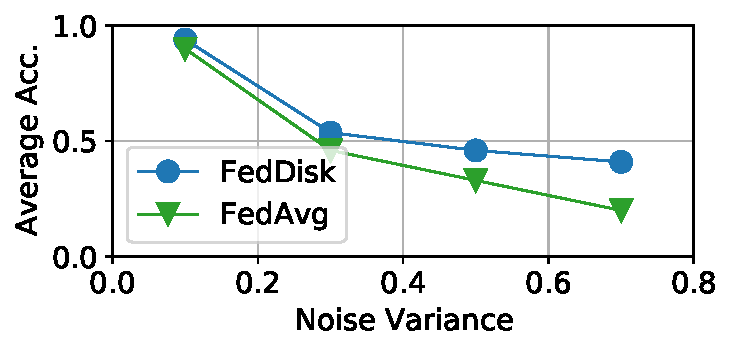
\includegraphics[width=0.8\linewidth]{\ChapterPathFedDisk/Figures/Accuracy_vs_noise}
	\caption[Accuracy over different noise levels.]{FedDisk and FedAvg accuracy on different added noise variance.}	
	\label{fig:accvsnoise}
\end{figure*}

\subsubsection{Communication Cost}
To evaluate the communication cost, we calculate the number of ``Effective Communication Rounds" (ECR). For \MethodnameShort{}, ECR include the communication rounds for exchanging MADE models and classification models. Figure \ref{fig:made_loss} show the aggregated training loss and validation loss for the global MADE model over communication rounds. The global MADE exchanging process stops when the validation loss starts increasing. For example, the proposed method needs 15 rounds for exchanging global MADE models in the case of FEMNIST dataset. The ECR for \MethodnameShort{} in the classification phase are calculated with the number of iterations that the proposed method needed to achieve the highest value of other methods gained. For example, for the FEMNIST dataset experiment shown in Figure \ref{fig:cl_acc_femnist}, \MethodnameShort{} only needs 105 rounds to reach the accuracy of 57\% (FedROD's accuracy), which is the highest accuracy among other experimental methods. Plus 15 rounds to exchange MADE model, \MethodnameShort{} only needs a total of 120 rounds to effectively reach the top comparison method accuracy. The ECRs of other methods are calculated with the number of exchanging classification model rounds until they reach their highest accuracy values.  

\begin{figure*}[ht!]
	\centering
	%[trim=left bottom right top, clip]
	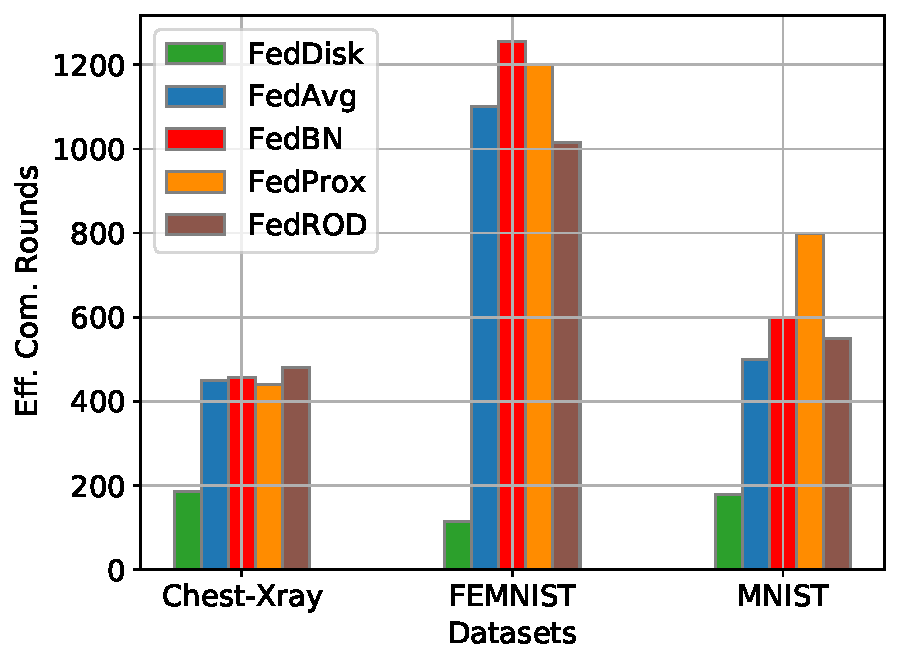
\includegraphics[width=0.85\linewidth]{\ChapterPathFedDisk/Figures/Com.Rounds}
	\caption[Summary of effective communication rounds.]{Summary of ``Effective Communication Rounds" over 3 datasets. The Figure shows that \MethodnameShort{} is much more efficient in terms of communication cost.}	
	\label{fig:communication_round}
\end{figure*}


Figure \ref{fig:communication_round} shows the summary of ``Effective Communication Rounds" for the three experimental datasets. As shown in the Figure, \MethodnameShort{} is the most effective method as it needs a lot fewer communication rounds to reach the highest accuracy among other methods. This is because the proposed method only needs a few number communication rounds for the global MADE model to be converged, and such statistical information accelerates the global classification model to reach high accuracy much faster compared to others. For example, for FEMNIST dataset, the \MethodnameShort{}'s ECR is only 120 (15 for MADE model exchange plus 105 for classification model exchange ), whereas others take more than 1000 iterations (a communication cost reduction of more than eight times). The communication cost reduction trend is also applied to other experimental datasets, Chest-Xray (2 times) and MNIST (2.5 times). Therefore, the proposed method not only improves the accuracy but also dramatically reduces the communication cost for the experimental datasets, which is one of the most critical concerns in Federated Learning.


\section{Conclusion}
\label{sec:FedConclusion}
In this work, we have proposed a FL method to tackle the issue of distribution skewed data. The technique utilizes a FL framework and a neural network-based density estimation model to derive training sample weights. This helps to adjust the global distribution without revealing clients' raw data. We also provide a privacy analysis for the extra information used in \MethodnameShort{} (i.e., the parameters of MADE models) and prove that the leakage information becomes less important when the number of clients increases. The experimental results show that the proposed method not only improves the FL accuracy but also significantly reduces communication costs. 
















	


\newcommand{\argmax}{{\operatorname{arg}\,\operatorname{max}}\;}
%\newcommand{\x}{$\times$}
\newcommand{\multirot}[3]{\multirow{#1}{*}{\rotatebox{#2}{ #3 } }}  %paras: rows,degree,text 


\DeclarePairedDelimiterX{\infdivx}[2]{(}{)}{%
	#1\;\delimsize\|\;#2%
}
\newcommand{\KL}{KL\infdivx}
\DeclarePairedDelimiter{\norm}{\lVert}{\rVert}

%\DeclareMathOperator*{\argmin}{\arg\min} 

\newcommand{\MethodnameLongSIMPOR}{Synthetic Information towards Maximum Posterior Ratio}
\newcommand{\Methodname}{SIMPOR}

\newcommand{\ChapterPathSIMPOR}{Chapter3}
\chapter{Synthetic Information Towards Maximum Posterior Ratio for Deep Learning on Class Imbalanced Data}
\label{chap:SIMPOR}



\section{Introduction}
Class imbalance is a common phenomenon; it could be caused by the data collecting procedure or simply the nature of the data. For example, it is difficult to sample some rare diseases in the medical field, so collected data for these are usually significantly less than that for other diseases. This leads to the problem of class imbalance in machine learning. The chance of rare samples appearing in model training process is much smaller than that of common samples. Thus, machine learning models tend to be dominated by the majority class; this results in a higher prediction error rate. Existing work also observed that class imbalanced data cause a slow convergence in the training process because of the domination of gradient vectors coming from the majority class \cite{ya-guan_emsgd:_2020, liu_high-performance_2020}. 

In the last decades, a number of techniques have been proposed to soften the negative effects of class imbalance for conventional machine learning algorithms by analytically studying particular algorithms and developing corresponding strategies. However, the problem for heuristic algorithms such as deep learning is often more difficult to tackle. As suggested in the most recent deep learning with class imbalance survey \cite{johnson_survey_2019}, most of the works are emphasizing image data, and studies for other data types are missing. Thus, in this work, we focus on addressing the issue of tabular data with class imbalance for deep learning models. We propose a class balancing solution that utilizes entropy-based sampling and data statistical information. As suggested in the survey (\cite{johnson_survey_2019}) that techniques for traditional ML can be extended to deep learning and inspiring by the comparison in a recent relevant work, Gaussian Distribution Based Oversampling (GDO) \cite{bib:GDO}, we compare the proposed technique with other widely-used and recent techniques such as GDO \cite{bib:GDO}, SMOTE \cite{chawla_smote:_2002}, ADASYN \cite{ADASYN}, Borderline SMOTE \cite{bordersmote}, Random Oversampling (ROS). 

We categorize existing solutions into model-centric and data-centric approaches in which the first approach aims at modifying machine algorithms, and the latter looks for data balancing techniques. Perhaps data-centric techniques are more commonly used because they do not tie to any specific model. In this category, a simple data balancing technique is to duplicate minority instances to balance the sample quantity between classes, namely random oversampling (ROS). This can preserve the best data structure and reduce the negative impact of data imbalance to some degree. However, this puts too much weight on a very few minority samples; as a result, it causes over-fitting problems in deep learning when the imbalance ratio becomes higher. 

Another widely-used technique in this category is Synthetic Minority Oversampling Technique (SMOTE) \cite{chawla_smote:_2002}, which randomly generates synthetic data on the connections (in Euclidean space) between minority samples. However, this easily breaks data topology, especially in high-dimensional space, because it can accidentally connect instances that are not supposed to be connected. In addition, if there are minority samples located in the majority class, the technique will generate sample lines across the decision boundary, which leads to distorted decision boundaries and misclassification. To improve SMOTE, Hui Han, \textit{et al.} \cite{bordersmote} proposed a SMOTE-based technique (Borderline SMOTE), in which they only apply SMOTE on the near-boundary samples determined by the labels of their neighbors. For example, if a sample Euclidean space-based group includes samples from other classes, they can be considered samples near the border. Since this technique is entirely based on Euclidean distance from determining neighbors to generating synthetic data, it performs poorly in high dimensional space. Similar to SMOTE, if there is any poorly generated sample near the boundary, it will worsen the problem due to synthetic samples bridges across the border. Leveraging the same way as SMOTE generates synthetic samples, another widely-used technique, ADASYN \cite{ADASYN}, controls the number of generated samples by the number of samples in different classes within small groups. Again, this technique still suffers distortion of the decision boundary if the boundary region is class imbalanced. Additionally, such mentioned techniques have not utilized statistical data information. A recent work, Gaussian Distribution Based Oversampling (GDO) \cite{bib:GDO}, balances data class based on the statistical information of data instead. However, its strong assumption of data distribution (data follow Gaussian) reduces the technique's effectiveness in real data.  

To alleviate the negative effects of data imbalance and avoid the drawbacks of existing techniques, we propose a minority oversampling technique that focuses on balancing the high-entropy region that provides the most critical information to the deep learning models. Besides, the technique enhances synthetic data's chance to fall into the minority class to reduce model errors. By carefully generating synthetic data near minority samples, our proposed technique also preserves the best data topology. Besides, our technique does not need any statistical assumption. 

To find informative samples, we leverage an entropy-based deep active learning technique that is able to select samples yielding high entropy to deep learning models. We denote the location of informative samples as the informative region. We then balance this region first, and the remaining data are balanced later so that it would reduce the decision distortion mentioned earlier. For each minority sample in this region, we safely generate its synthetic neighbors so that the global data topology is still preserved. However, generating synthetic samples in this region is risky because it can easily fall across the decision boundary. Therefore, we find a direction to generate synthetic samples by maximizing their posterior probability based on Bayes's Theorem. However, maximizing the posterior probability is facing infeasible computation in the denominator. To overcome this, we maximize the posterior ratio instead so that the denominator computation can be avoided. This also ensures that the synthetic samples are not only close to the minority class but also far from the majority class. The remaining data are eventually balanced by a similar procedure. 

The proposed technique alleviates the class imbalance problem. Our experiments indicate that we can achieve better classification results over widely-used techniques in all experimental cases by applying the proposed strategy.  

Our work has the following main contributions:
\begin{enumerate}
	\item{Exploring the impact of class imbalance mitigations on deep learning via visualization and experiments.}
	\item{Proposing a new minority oversampling-based technique, namely \MethodnameLongSIMPOR, to balance data classes and alleviate data imbalance impacts. Our technique is enhanced by the following key points.}
	\begin{enumerate}
		\item Leveraging an entropy-based active learning technique to prioritize the region that needs to be balanced. It is the informative region where samples provide high information entropy to the model. 
		\item Leveraging Maximum Posterior Ratio and Bayes's theorem to determine the direction to generate synthetic minority samples to ensure the synthetic data fall into the minority class and not fall across the decision boundary. To our best knowledge, this is the first work utilizing the posterior ratio for tackling class imbalanced data. 
		\item Approximating the likelihood in the posterior ratio using kernel density estimation, which can approximate a complicated topology. Thus, the proposed technique is able to work with large, distributively complex data. 
		\item Carefully generating synthetic samples surrounding minority samples so that the global data topology is still preserved. 
	\end{enumerate}
	\item{We applied our technique to 41 real datasets with a diversity of imbalance ratio and the number of features.}
	\item{We compare our technique with different widely-used and recent techniques. The results show that the proposed technique outperforms others.}
\end{enumerate}


The rest of this paper is organized as follows. Section \ref{sec:preliminaries} introduces related concepts that will be used in this work, i.e., Imbalance Ratio, Macro F1-score, AUC, and Entropy-based active learning. Section \ref{sec:problem} will provide more detail on the problem of learning from an imbalanced dataset. Our proposed solution to balance dataset, \MethodnameLongSIMPOR, will be explained comprehensively in Section \ref{sec:SIMPOR_method}. Section \ref{sec:implementation} discusses the technique implementation and complexity. We will show experiments on different datasets, including artificial and real datasets in Section \ref{sec:experiments}. We also discuss experimental results in the same section. In Section \ref{sec:relatedwork}, we briefly review other existing works. Section \ref{sec:conclusion} concludes the study and discusses future work. 

\section{Preliminaries}
\label{sec:preliminaries}       
In this section, we introduce related concepts that will be used in our work. 

\subsection{Imbalance Ratio (IR)}
For binary classification problems, we use imbalance ratio (IR) to depict the data imbalance as it has been widely used. IR is the ratio of the majority class samples to the minority class's samples. For example, if a dataset contains 1000 class-A and 100 class-B samples, the Imbalance Ratio is 10:1.   

\subsection{Evaluation Metrics}
\label{f1score}
In this work, we evaluate balancing data techniques by classification performance. Specifically, we use F1-Score and Area Under the Curve (AUC) as evaluation metrics. We measure the Macro-averaging for measuring F1-scores in which we compute scores per class and take the average of all classes with the same weight regardless of how often they appear in the datasets. These are fair measurements for imbalanced test datasets. 

F1 score is computed based on two factors Recall and Precision as follows:

\begin{align}
Recall &= \frac{TP}{TP+FN}\\
Precision &= \frac{TP}{TP+FP}\\
F1-score &= \frac{2*Recall*Precision}{Recall+Precision},
\end{align}
where $T$ and $F$ stand for True and False; $P$ and $N$ stand for Positive and Negative. 

We also measure AUC \cite{cite:AUC} scores as it is an important metric to evaluate imbalanced data. AUC is derived from Receiver Operating Characteristic curve (ROC). In this work, we utilize a skit-learn library to compute AUC; the library can be found in sklearn.metrics.auc. 


\subsection{Entropy-based Active Learning }   
\label{sec:EAL}
To find informative samples, we leverage entropy-based active learning. The technique gradually selects batch-by-batch samples that provide high information to the model based on information entropy theory \cite{shannon_mathematical_1948}. The information entropy is quantified based on the ``surprise" to the model in terms of class prediction probability. Take a binary classification, for example, if a sample is predicted to be 50\% belonging to class A and 50\% belonging to class B, this sample has high entropy and is informative to the model. In contrast, if it is predicted to be 100\% belonging to class A, it is certain and gives zero information to the model. The class entropy $E$ for each sample can be computed as follows. 

\begin{equation}
E(x,\theta) = -\sum_i^n{ P_\theta( y=c_i|x) \log_n P_\theta(y=c_i|x) }
\label{eq:entropy_AL}
\end{equation} 
where $P_\theta(y=c_i|x)$ is the probability of data $x$ belonging to the \textit{i}th class of $n$ classes with current model parameter $\theta$.

In this work, we consider a dataset containing $N$ pairs of samples $X$ and corresponding labels $y$, and a deep neural network with parameter $\theta$. At the first step $t^{(0)}$, we train the classifier with parameter $\theta^{(0)}$ on a random batch of $k$ labeled samples and use the $\theta^{(0)}$ to predict the labels for the rest of the data (we assume their labels are unknown). We then compute the prediction entropy of each sample based on Equation \ref{eq:entropy_AL}. We are now able to collect the first batch of informative samples by selecting $k$ samples based on the top $k$ highest entropy. We query labels for this batch and concatenate them to existing labeled data to train the classifier parameter $\theta^{(1)}$ in the next step $t^{(1)}$. Steps are repeated until the number of informative samples reaches a pre-set informative portion (IP). For example, $IP=0.3$ will select the top 30\% high entropy samples as informative samples.  

\section{The Problem of Learning From Imbalanced Datasets}
\label{sec:problem}
In this section, we review the problem of learning from imbalanced datasets. Although the problem may apply to different machine learning methods, we focus on deep learning in this work. 

\begin{figure}[t!]
	%[trim=left bottom right top, clip]
	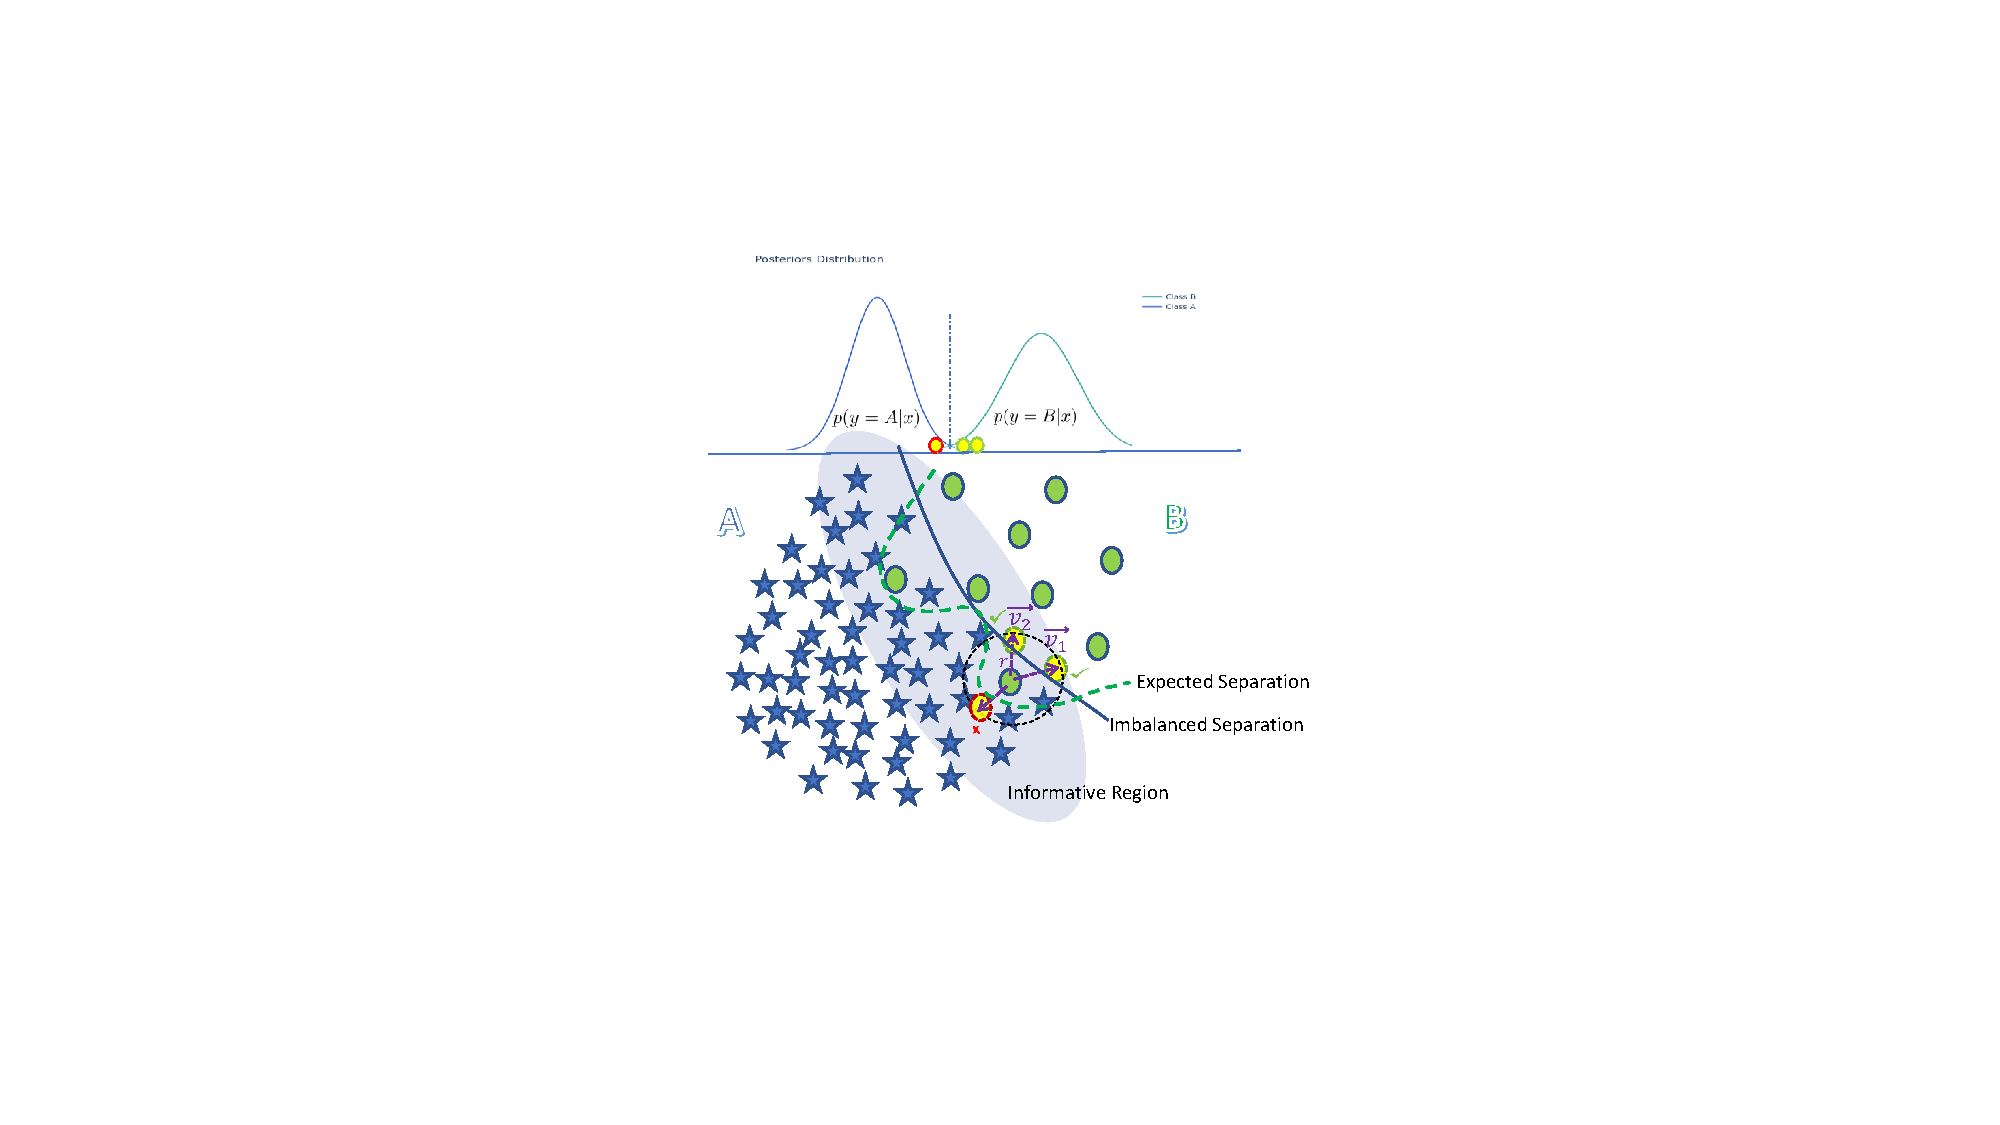
\includegraphics[width=\linewidth, trim=300 150 310 120,clip]{\ChapterPathSIMPOR/Figures/proplem.pdf}
	\caption{Learning from imbalanced datasets}
	\label{fig:problem}
\end{figure}

Figure \ref{fig:problem} illustrates our problem on a binary classification. The imbalance in the informative region (light blue eclipse) could lead to classification errors. The dashed green line depicts the expected boundary, while the solid blue line is the model's boundary. Since the minority class lacks data in this region, the majority class will dominate the model even with a few noisy poorly-placed samples, which leads to a shift of the model's boundary. In contrast to the study by Ertekin \textit{et al.} \cite{ertekin_learning_2007} which assumes the informative region is more balanced by nature and proposes a solution that only classifies over the informative samples, our assumption is different. We consider the case that the informative region contains highly imbalanced data, which we believe happens in most real scenarios. The problem could be more severe in a more complex setting such as high-dimensional and topologically complex data. Therefore, we proposed a technique to tackle the problem of data imbalance by oversampling the minority class in an informative manner. The detail of our proposed technique will be described in Section \ref{sec:SIMPOR_method}.   
       



\section{Related Work}
\label{sec:relatedwork}
In the last few decades, there have been a number of solutions proposed to alleviate the negative impacts of data imbalance in machine learning. However, many of them are not efficient when it comes to high-dimensional data and deep learning. In this section, we review algorithms that aim at deep learning and strategies inherited from conventional machine learning methods. These techniques can mainly be categorized into two different categories, i.e., data-centric and model-centric approaches. 


Model-centric approaches usually require modifications of algorithms on the cost functions in order to balance the weight of each class. Specifically, such cost-sensitive approaches put higher penalties on majority classes and less on minority classes to balance their contribution to the final cost. For example,  \cite{cui_class-balanced_2019} provided their designed formula $ (1 - \beta^n)/(1 - \beta)$ to compute the weight of each class based on the effective number of samples $n$ and a hyperparameter $\beta$ which is then applied to re-balance the loss of a convolutional neural network model.  \cite{huang_learning_2016},\cite{rangarajan_sridhar_unsupervised_2015}, \cite{DBLP:journals/corr/abs-1805-00932} assign classes' weights inversely proportional to sample frequency appearing in each class.      


Compared to model-centric-based manners, data-centric approaches have been attracting more research attention as it is independent of machine learning algorithms. In this category, we divide into two main approaches, i.e. sampling-based and generative approaches. Sampling-based methods \cite{DBLP:journals/corr/ShenLH15}, \cite{DBLP:journals/corr/abs-1711-00941}, \cite{haibo_he_learning_2009}, \cite{li_entropy-based_2020}, \cite{ertekin_active_2007} mainly generate a balanced dataset by either over-sampling minority classes or down-sampling majority classes. Some methods are not designed for deep learning, but we still consider them since they are independent of the machine learning model architecture. In a widely used method SMOTE \cite{chawla_smote:_2002}, Chawla \textit{et al.} attempt to oversampling minority class samples by connecting an sample to its neighbors in feature space and arbitrarily drawing synthetic samples along the connections. However, one of the drawbacks of SMOTE is that if there are samples in the minority class located in the majority class, it creates synthetic sample bridges towards the majority class \cite{goswami_class_2020}. This renders difficulties in differentiation between the two classes. Another SMOTE-based work namely Borderline-SMOTE \cite{bordersmote} was proposed in which its method aims to do SMOTE with only samples near the border between classes. The samples near the border are determined by the labels of its \textit{k} distance-based neighbors (if more than half of neighbors belong to the other class, the sample is considered to be on the border). This "border" idea is similar to ours to some degree. However, finding a good \textit{k} is critical, and it is usually highly data-dependent. In addition, Borderline-SMOTE again faces the problems of SMOTE. 


Under the down-sampling category, other works \cite{ertekin_learning_2007}, \cite{aggarwal_active_2020} leverage active learning techniques to find informative samples which authors believe the imbalance ratio in these areas is much smaller than that in the entire dataset. They then classify this small pool of samples to improve the performance and expedite the training process for the SVM-based method. however, this method was only designed for SVM-based methods which mainly depend on the support vectors. Also, this potentially discards important information of the entire dataset because only a small pool of data is used.  

Generative approaches which generate synthetic samples in minor classes by sampling from data distribution are becoming more attractive as they are outperforming other methods in high dimensional data \cite{DBLP:conf/dmin/LiuGM07}. When it comes to images, a number of deep learning generative-based methods have been proposed as deep learning is capable of capturing good image representations. \cite{rashid_convergence_2012} \cite{dai_generative_2019} \cite{mullick_generative_2019} utilized Variational Autoencoder as a generative model to arbitrarily generate images from learned distributions. However, most of them assumed simple prior distributions such as Gaussian for minor classes, they tend to simplify data distribution and might not succeed in sophisticated distributions. Our solution also falls into this category; however, we leverage the idea of a mixture model to tackle this issue for image data.     



\section{Methodology}
\label{sec:SIMPOR_method}
To alleviate the negative effects of data imbalance, we propose a comprehensive approach, \MethodnameLong{} (\Methodname), which aims to generate synthetic samples for minority classes. First, the informative region that contains informative samples is determined and balanced by creating surrounding synthetic neighbors for minority samples. The remaining region is then fully balanced by arbitrarily generating minority samples' neighbors. The remainder of this section provides further information about how our approach was developed.  

\subsection{Methodology Motivation}  
As Chazal and Michel mentioned in their work \cite{leroueil_compressibility_1996}, the natural way to highlight the global topological structure of the data is to connect data points' neighbors; our proposed method aligns with their observation by generating surrounding synthetic neighbors for minority samples to preserve data topology. Thus, our technique not only generates more data for minority class but also preserve the underlying topological structure of the entire data. 

Similar to \cite{ertekin_learning_2007} and \cite{aggarwal_active_2020}, we believe that informative samples play the most important role in the prediction success of both traditional machine learning models (e.g., SVM, Naive Bayes) and modern deep learning approaches (e.g., neural network). Thus, our technique finds these informative samples and focuses on augmenting minority data in this region. In this work, an entropy-based active learning strategy mentioned in \ref{sec:EAL} is applied to find the samples that contain more information to the model. This strategy is perhaps the most popular active learning technique and over-performs many other techniques on several datasets \cite{DAL}, \cite{7393573} \cite{settles_analysis_2008}.

\subsection{Generating minority synthetic data}  
\label{sec:solvingOptimization}
\R{1.1a}
\Copy{1.1a}{
A synthetic neighbor $ x'$ and its label $y'$ can be created surrounding a minority sample $x$ by adding a small random vector $v$ to the sample, $x' = x + v$. Thus, $x'$ can be selected on the d-sphere's surface centered at $x$ with a radius of $|\vec{v}|$. For notation convenience, let $r = |\vec{v}|$ be the radius of the d-sphere. To enrich the synthetic samples, $r$ is sampled from a defined Gaussian distribution to generate a new synthetic sample distance each time. This section describes how the direction and distance of a synthetic sample are determined, which can also be represented via the direction and length of vector $\vec{v}$.

It is critical to generate synthetic data in the informative region because synthetic samples can unexpectedly jump across the decision boundary. This can be harmful to models as this might create outliers and reduce the model's performance. Therefore, we safely find vector $\vec{v}$ towards the minority class, such as $\vec{v}_0$ and $\vec{v}_1$ depicted in Figure \ref{fig:problem}.} Our technique is described via a binary classification scenario as follows. 

Let's consider a binary classification problem between majority class A and minority class B. 
From the Bayes' theorem, the posterior probabilities $p(y'=A|x')$ or $p(y'=B|x')$ can be used to present the probabilities that a synthetic sample $x'$ belongs to class A or class B, respectively. Let the two posterior probabilities be $f_0$ and $f_1$; they can be expressed as follows. 
\begin{align}
	\label{eq:posterior}
	p(y'=A|x') = \frac{p(x'|y'=A)\:p(A)}{p(x')} = f_0 \\
	p(y'=B|x') = \frac{p(x'|y'=B)\:p(B)}{p(x')} = f_1  
\end{align}

As mentioned earlier, each synthetic data $x'$ is generated so that it maximizes the probability of $x'$ belonging to the minority class $B$ and minimizes the chance $x'$ falling into the majority class $A$. Thus, a technique that maximizes the fractional posterior $f$ is proposed,   
\begin{align}
	\label{eq:fracpost}
	f &= f_1/f_0  \\
	&=\frac{p(x'|y'=B) \:p(B)}{p(x'|y'=A) \: p(A)}. \label{equ:f_ratio}
\end{align}


\textbf{\textit{Approximation of likelihoods in Equation \ref{equ:f_ratio}:}} A non-parametric kernel density estimates (KDE) is selected to approximate the likelihoods $p(x'|y'=A)$ and $p(x'|y'=B)$ as KDE is flexible and does not require specific assumptions about the data distribution. One can use a parametric statistical model such as Gaussian to approximate the likelihood; however, it oversimplifies the data and does not work effectively with topological complex data, especially in high dimensions. In addition, parametric models require an assumption about the distribution of data which is difficult in real-world problems since we usually do not have such information. On the other hand, KDE only needs a kernel working as a window sliding through the data. Among different commonly used kernels for KDE, we choose Gaussian Kernel as it is a powerful continuous kernel that would also eases the derivative computations for finding optima.
 
\R{PriorApproximation}
\Copy{PriorApproximation}{
\textbf{\textit{Approximation of priors in Equation \ref{equ:f_ratio}:}} Additionally, we estimate the prior probabilities of observing samples in class A ($p(A)$) and class B ($p(B)$) (in Equation \ref{equ:f_ratio}) by the widely-used Empirical Bayes Method \cite{empiricalBayes} to leverage the existing information from the original data. The estimates are denoted as $\widehat{p(A)}$ and $\widehat{p(B)}$ respectively.

\textbf{\textit{Equation \ref{equ:f_ratio} Approximation:} } Let $X_A$ and $X_B$ be the subsets of dataset $X$ which contain samples of class A and class B, $X_A=\{x: y=A  \}$ and $X_B=\{x: y=B  \}$. $N_A$ and $N_B$ are the numbers of samples in $X_A$ and $X_B$. $d$ is the number of data dimensions. $h$ presents the width parameter of the Gaussian kernel. The posterior ratio for each synthetic sample $x'$ then can be estimated as follows:

\begin{align}
	\label{eq:fracpost_estimation}
	f &= \frac{p(x'|y'=B)  \: p(B)}{p(x'|y'=A) \: p(A)} \\
	&\propto \frac{ \frac{1}{N_B h^d} \: \sum_{i=1}^{N_B}{ (2\pi)^{-\frac{d}{2}} \: e^{\frac{1}{2}{(\frac{x'-X_{B_i}}{h})^2} } } \: \widehat{p(B)} }
	{ \frac{1}{N_A h^d} \:  \sum_{j=1}^{N_A}{ (2\pi)^{-\frac{d}{2}} \: e^{ \frac{1}{2} {(\frac{x-X_{A_j}}{h})^2} } }\: \widehat{p(A)} }\\
	& \propto \frac{ \frac{1}{N_B h^d} \: \sum_{i=1}^{N_B}{ \: e^{\frac{1}{2}{(\frac{x'-X_{B_i}}{h})^2} } } \: \widehat{p(B)} }
	{ \frac{1}{N_A h^d} \:  \sum_{j=1}^{N_A}{  \: e^{ \frac{1}{2} {(\frac{x-X_{A_j}}{h})^2} } }\: \widehat{p(A)} }
	\label{equ:f}
\end{align} 
}


\textbf{\textit{Selecting bandwidth parameter $h$ for Gaussian kernel:} } The bandwidth is automatically selected for each dataset using the most common method, namely Scott's rule of thumb, proposed by Scott \cite{scott_2015}. With an attempt to minimize the mean integrated squared error, the parameter is estimated as $h = N^{(-\frac{1}{d+4})}$ where $N$, $d$ are the number of data points and the number of dimensions respectively. This study utilizes a scikitlearn python library for KDE, including bandwidth selection. The implementation detail can be found at \cite{skitlearnKDE}. 

\R{1.1b}
\textbf{\textit{Finding synthetic samples surrounding a minority sample:}} To generate neighbors for each minority sample that maximizes Function \text{f} in Equation \ref{equ:f}, points on each $r$-radius sphere centered at a minority sample are considered synthetic instances. As a result, a vector $\vec{v}$ can be added to a minority sample for generating a new instance. \Copy{1.1b}{The relationship between a synthetic sample $x'$ and a minority sample can be described as follows,
\begin{align}
	\label{equ:vecV}
	\vec{x'} =  \vec{x} + \vec{v},
\end{align}
where the length of $\vec{v}$ is equal to $r$, and $r$ is sampled from a Gaussian distribution,
\begin{align}
     r \sim \mathcal{N}(0,\,(\alpha R)^{2}),
     \label{equ:r_dist}
\end{align}
where $\alpha R$ is the standard deviation of the Gaussian distribution and $ 0< \alpha <=1 $.
The range parameter $R$ is relatively small and computed as the average distance of a minority sample $x$ to its k-nearest neighbors. This will ensure that the generated sample will surround the minority sample. The Gaussian distribution with the mean of zero and the standard deviation $\alpha R$ controls the distance between the synthetic samples and the minority sample. The standard deviation is tuned from 0 to R by a coefficient $\alpha \in (0,1]$. The larger the $\alpha$ is, the farther synthetic data is placed from its original sample.} Consider a minority sample $x$ and its k-nearest neighbors in the Euclidean space, $R$ can be computed as follows:

\begin{align}
	R = \frac{1}{k}\sum\limits_{1}^{k} ||x-x_j ||,
\end{align}
where $||x-x_j||$ is the Euclidean distance between a minority sample $x$ and its $j$th neighbor. $k$ is a parameter indicating selected number of neighbors. 


\begin{figure}[th]
	%[trim=left bottom right top, clip]
	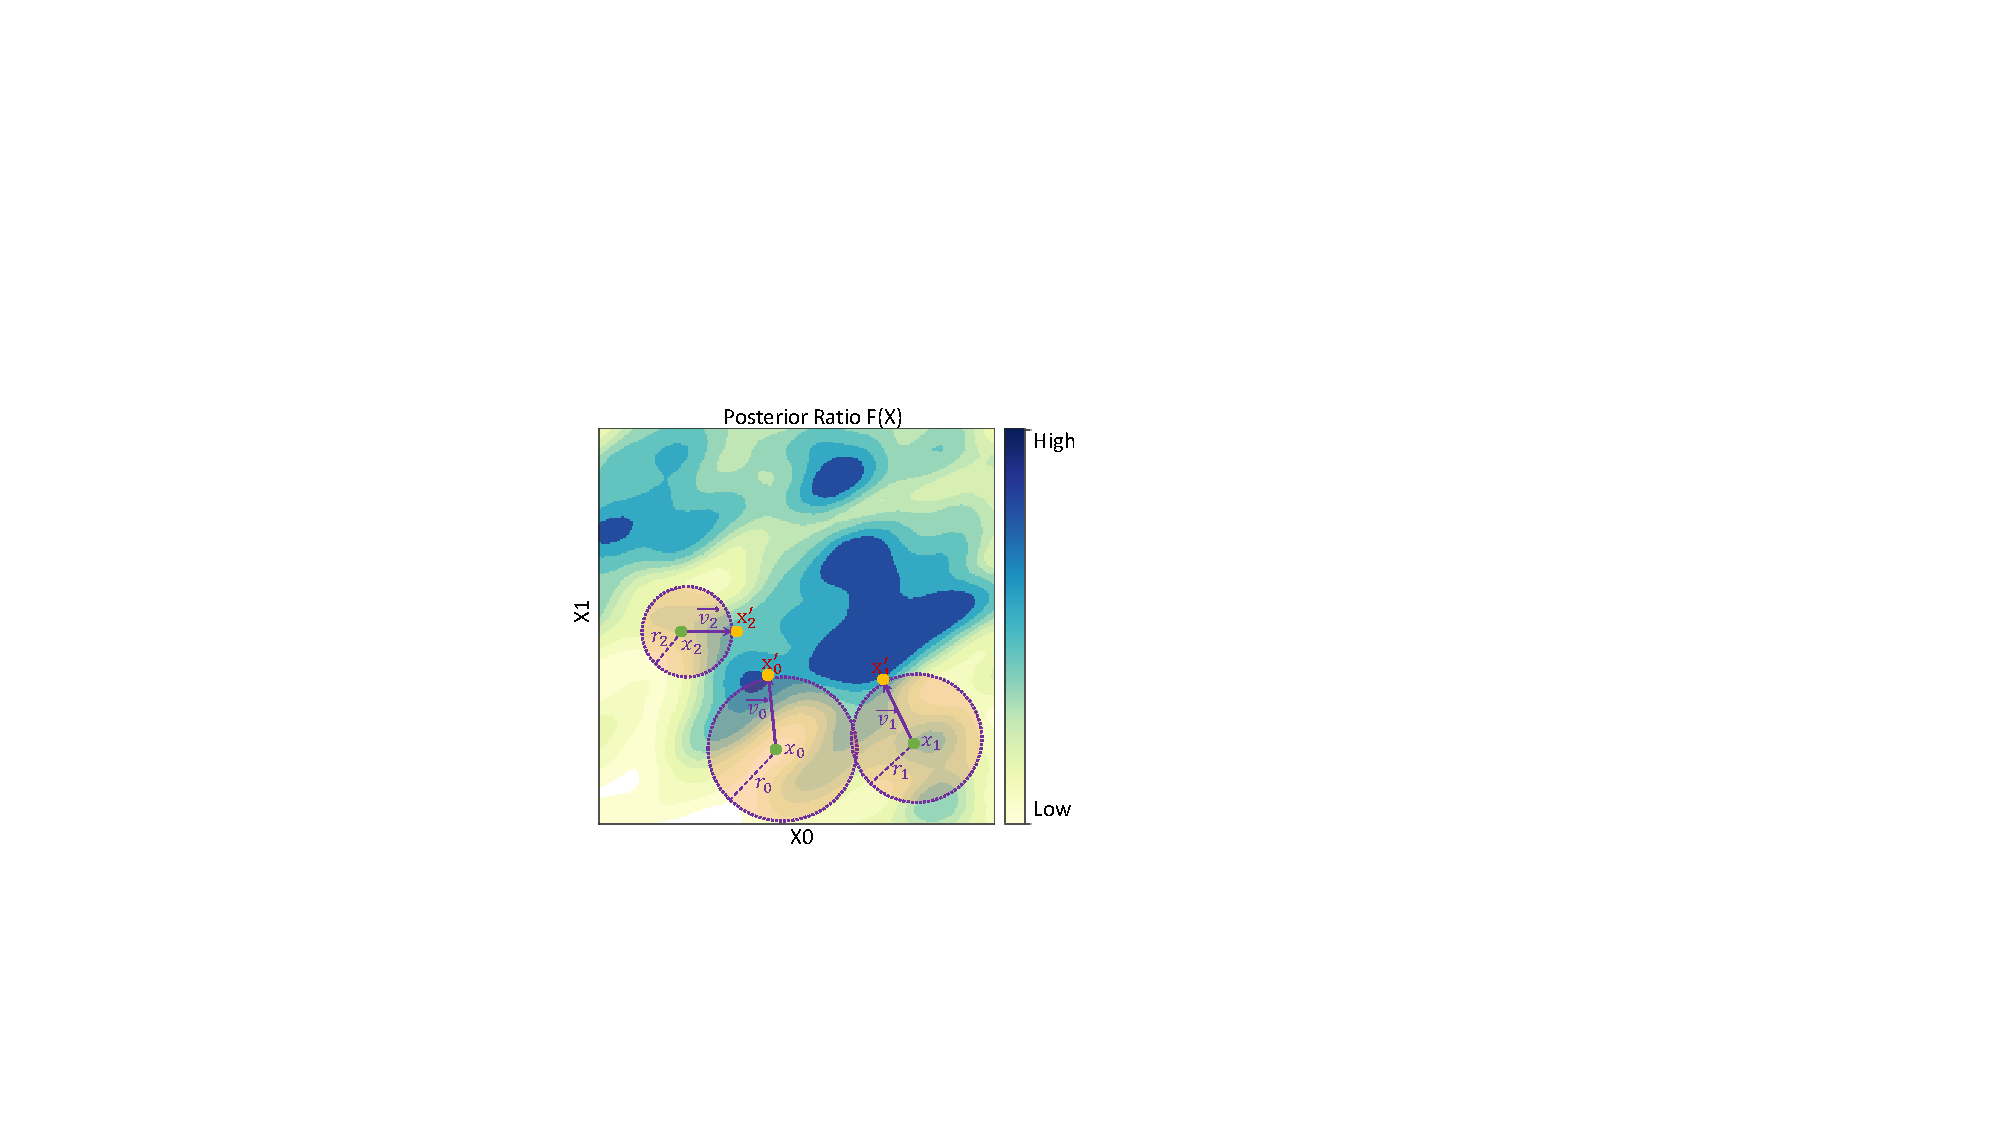
\includegraphics[width=\linewidth, trim=240 120 390 160,clip]{Figures/MaxPosteriorRatio/sphere_maxF.pdf}
	\caption{Demonstration on how \Methodname{} generates three synthetic samples $x'_0, x'_1, x'_2$, from three minority samples $x_0, x_1, x_2$, by maximizing the Posterior Ratio. }
	\label{fig:sphere_maxF}
\end{figure}

Figure \ref{fig:sphere_maxF} depicts a demonstration of finding 3 synthetic samples from 3 minority samples. In practice, one minority can be re-sampled to generate more than one synthetic samples. For a minority sample $x_0$, we find a synthetic sample $x_0'$ by maximizing the objective function $f(x_0'), x_0' \in X$ with a constraint that the Euclidean length of $\vec{v_0}$ equals to a radius $r_0$, $||\vec{v_0}|| = r_0$ or $||\vec{x_0'}-\vec{x_0}||=r_0$ (derived from Equation \ref{equ:vecV}). 


The problem can be described as a constrained optimization problem. For each minority sample $x$, we find a synthetic sample $x'\in \mathbb{R}^d$ lying on the d-sphere centered at $x$ with radius $r$ and maximizing function in Equation \ref{equ:f},
\begin{align}
	\label{prob:optimazation}
	\max_{x'} {f(x')} \;\;\; \textrm{s.t.}\; ||\vec{x'} - \vec{x}||=r.
\end{align}

\textbf{\textit{Solving optimization problem in Equation \ref{prob:optimazation}:}} Interestingly, the problem in Equation\ref{prob:optimazation} can be solved numerically. Function $f(x)$ in Equation \ref{equ:f} is defined and continuous for $x' \in (-\infty, +\infty)$ because all of the exponential components (Gaussian kernels) are continuous and greater than zero. In addition, the constraint, $||\vec{x'} - \vec{x}||=r$, which contains all points on the sphere centered at $x$ with radius $r$ is a closed set (\cite{wikipedia_2021}). Thus, a maximum exits as proved in \cite{maximum_exist}. To enhance the diversity of synthetic data, either the global maximum or any local maximum can be accepted so that the synthetic samples will not simply go to the same direction.  

We solve the problem in Equation \ref{prob:optimazation} by using the Projected Gradient Ascent approach in which we iteratively update the parameter to go up the gradient of the objective function. A local maximum is found if the objective value cannot be increased by any local update. For simplification, we rewrite the problem in Equation \ref{prob:optimazation} by shifting the origin to the considered minority sample. The problem becomes finding the maximum of function $f(x')$, $x' \in \mathbb{R}^d$, constrained on a d-sphere, i.e., $||x'||=r$. Our solution can be described in Algorithm \ref{alg:optimization}. After shifting the coordinates system, we start by sampling a random point on the constraint sphere (line $1-2$). The gradient of the objective function at time $t$, $g_t(x'_t)$, is computed and projected onto the sphere tangent plane as $p_t$ (line $4-5$). It is then normalized and used for update a new $x'_{t+1}$ by rotating a small angle $lr*\theta$ (line $6-7$). The algorithm stops when the value of $f(x')$ is not increased by any update of $x'$. We finally shift to the original coordinates and return the latest $x'_t$.   
\begin{algorithm}[ht]
	\caption{Sphere-Constrained Gradient Ascent for Finding Maximum}
	
	\begin{flushleft}
		\textbf{Input}: A minority sample $x_0$, objective function $f(x,X)$\\
		\textbf{Parameter}: \\
		$r$ : The radius of the sphere centered at $x_0$  \\\
		$\theta$ : Sample space $\theta \in [0,2\pi]$ \\
		$lr$ : Gradient ascent learning rate\\
		
		\textbf{Output}: An local maximum $x'$\\
		\begin{algorithmic}[1]
			\STATE Shift the Origin to $x_0$
			\STATE Randomly initiate $x'_t$ on the sphere with radius $r$	
			\WHILE {converge condition}
			\STATE Compute the gradient at $x'_t$\\
			$g_t(x'_t) = \nabla f(x'_t)$
			\STATE Project the gradient onto the sphere tangent plane\\
			$p_t = g_t - (g_t \cdot x'_t) x_t$
			\STATE Normalize projected vector\\
			$p_t = p_t/ ||p_t||$
			\STATE Update $x'$ on the constrained sphere \\
			$x'_{t+1} = x'_t cos(lr*\theta) + p_t sin (lr*\theta)$ 			
			\ENDWHILE
			\STATE Shift back to the Origin
			\RETURN $x'_t$
		\end{algorithmic}
	\end{flushleft}
	\label{alg:optimization}
\end{algorithm}


\textbf{\textit{Avoiding synthesis of noise:}} To reduce the chance of misplacing synthetic samples on another class region because of noisy borderline and mislabeled minority samples, we set a policy for rejecting minority candidates which are selected for oversampling. The idea is to reject candidates surrounded mainly by other class samples. More specifically, we count the labels of the candidate's $k$-nearest neighbors and reject this candidate if there exists a class that its' number of samples is greater than the number of the minority samples). For example, the candidate is rejected when a class-A sample is selected for generating synthetic data, and its 5-nearest neighbors contain four class-B samples and one class-A sample. This is to avoid selecting mislabeled samples and noisy borderline samples for oversampling.        

\subsection{Algorithm}
Our strategy can be described in Algorithm \ref{alg:SIMPOR}. The algorithm takes an imbalanced dataset as its input and results in a balanced dataset which is a combination of the original dataset and synthetic samples. We first choose an active learning method $AL(\cdot)$ and find a subset of informative samples $S$ by leveraging entropy-based active learning (lines $1-2$). We then generate synthetic data to balance $S$. For each random sample $x_i^c$ in $S$ and belonging to minority class $c$, we randomly sample a small radius $r$ and find a synthetic sample that lies on the sphere centered at $x_i^c$ and maximizes the posterior ratio in Equation \ref{equ:f} (lines $3-11$). The process is repeated until the informative set $S$ is balanced. Similarly, the remaining region is balanced, which can be described in the pseudo-code from line $12$ to line $20$. The final output of the algorithm is a balanced dataset $D'$.       

\begin{algorithm}[ht]
	\caption{\Methodname}
	
	\begin{flushleft}
		\textbf{Input}: Original Imbalance Dataset $D$ including data $X$ and labels $y$.\\
		\textbf{Parameter}: 
		$MA$ is the majority class, $MI$ is a set of other classes.\\
		$k$: Number of  neighbors of the considered sample which determines the maximum range of the sample to its synthetic samples.\\ 
		$\alpha$: preset radius coefficient
		$Count(c, P)$ : A function to count class $c$ sample number in population $P$.\\
		$G(x_0,f,r)$ : Algorithm \ref{alg:optimization}, which returns a synthetic sample on sphere centered at $x_0$ with radius $r$ and maximize Equation \ref{equ:f}.  \\
		\textbf{Output}: Balanced Dataset $D'$ including $\{X',y'\}$
		\begin{algorithmic}[1]
			\STATE Select an Active Learning Algorithm $AL()$
			\STATE Query a subset of informative samples $S \in D$  using $AL$:
			$s  \leftarrow AL(D) $	\\
			
			\COMMENT{Balance the informative region}
			\FOR {$c \in MI$}
			\WHILE {$Count(c, S) \leq Count(MA, S)$ }
			\STATE Select a random $x_i^c \in S$
			\STATE Reject and reselect $x_i^c$ if its label is dominated among k-nearest labels
			\STATE Compute maximum range $R$ based on k-nearest neighbors
			\STATE Randomly sample a radius $r \sim \mathcal{N}(0,\alpha R)$
			\STATE Generate a synthetic neighbor $x'$ from $x_i^c$:
			$x'=G(x_i^c,f,r)$ 
			\STATE Append $x'$ to $D'$
			\ENDWHILE
			\ENDFOR
			
			\COMMENT{Balance the remaining region}
			\FOR {$c$ in $MI$}
			\WHILE { $Count(c, D') \leq Count(MA, D')$ }	
			\STATE Select a random $x_j^c \in \{X-S\}$
			\STATE Compute maximum range $R$ based on $k$
			\STATE Randomly sample a radius $r \sim \mathcal{N}(0,\alpha R)$
			\STATE Generate a synthetic neighbor $x'$ of $x_j^c$ 
			\STATE Append $x'$ to $D'$
			\ENDWHILE
			\ENDFOR
			\RETURN 
		\end{algorithmic}
	\end{flushleft}
	\label{alg:SIMPOR}
\end{algorithm}



%\section{Algorithm Implementation and Time Complexity}


\section{Algorithm Time Complexity.}
\label{sec:implementation}


\iffalse
Our proposed technique is straightforward in implementation. We first train a neural network model with initial samples and start querying the next batches of data based on the entropy scores from the previous model to find informative samples. The model is then updated with new batches of data until the entropy scores reach a certain threshold. All the informative samples are then balanced first, and the remaining data are balanced later. Each synthetic data point is generated by finding local maxima in Equation \ref{equ:f}.
\fi

The costly part of \Methodname{} is that each synthetic sample requires computing a kernel density estimation of the entire dataset. Elaborately, let $n$ be the number of samples of the dataset. In the worst case, the numbers of samples of minority and majority class are $N_B = 1$ and $N_A = n-1$, respectively. We need to generate $n-2$ synthetic samples to balance the dataset completely. Since each generated sample must loop through the entire dataset of size $n$ to estimate the density, the algorithm complexity is $O(n^2)$. 

Although generating synthetic data is only a one-time process, and this does not affect the classification efficiency in the testing phase, we still try to alleviate its weakness by providing parallelized implementations to reduce the time complexity to $O(n)$. Specifically, each exponential component in Equation \ref{equ:f} is computed parallelly, utilizing GPU or CPU threads. Ellaborately, Equation \ref{equ:f} can be rewritten as $N_B$ components of $e^{\frac{1}{2} (\frac {x - X_{B_i}}{h})^2}$ and $N_A$ components of $e^{\frac{1}{2} (\frac {x - X_{A_i}}{h})^2}$. Fortunately, they are all independent and can be processed parallelly. Thus, with a sufficient hardware resource, the consumption time for the kernel density estimation of each synthetic data point is then reduced by $N_A+N_B=n$ times, which significantly simplifies the complexity to $O(n)$.






\section{Experiments}
\label{sec:experiments}
\R{sow}
\Copy{sow}{
In this section, we explore the techniques via binary classification problems on an artificial dataset (i.e., Moon) and 41 real-world datasets (i.e., KEEL, UCI, Credit Card Fraud) with a diversity of imbalance ratios and different numbers of features. Samples in Moon have two features, while other datasets contain various numbers of features and imbalance ratios.} Dataset details are described in Table \ref{tab:dataDecription}.  
The implementation steps to balance datasets follow Algorithm \ref{alg:SIMPOR}. To evaluate our proposed balancing technique, we compare the classification performance to different widely-used and state-of-the-art techniques. More specifically, We compare \Methodname{} to SMOTE \cite{chawla_smote:_2002}, Borderline-SMOTE \cite{bordersmote},  ADASYN \cite{ADASYN}, DeepSMOTE \cite{deepsmote}, Gaussian Distribution Based Oversampling (GDO) \cite{bib:GDO}, SVMCS \cite{cssvm}, EE \cite{EE}. To evaluate the classifications performance for skewed datasets, we measure widely-used metrics, i.e., F1-score and Area Under The Curve (AUC). 

% Table generated by Excel2LaTeX from sheet 'KEEL Data Description'
\Copy{datasetTable}{
\begin{table}[htbp]
	\centering
	\caption{Dataset Description.}
	
	\begin{tabular}{lccc}
		\hline
		dataset & \#samples & \#features & IR \bigstrut\\
		\hline
		glass1 & 214   & 9     & 1.8 (138:76)\bigstrut[t]\\
		wisconsin & 683   & 9     & 1.9 (444:239) \\
		pima  & 768   & 8     & 1.9 (500:268)\\
		glass0 & 214   & 9     & 2.1 (144:70) \\
		yeast1 & 1484  & 8     & 2.5 (1055:429)\\
		haberman & 306   & 3     & 2.8 (225:81) \\
		vehicle1 & 846   & 18    & 2.9 (629:217)\\
		vehicle2 & 846   & 18    & 2.9 (628:218)\\
		vehicle3 & 846   & 18    & 3.0 (634:212)\\
		creditcard & 1968  & 30    & 3.0 (1476:492)\\
		glass-0-1-2-3\_vs\_4-5-6 & 214   & 9     & 3.2 (163:51)\\
		vehicle0 & 846   & 18    & 3.3 (647:199)\\
		ecoli1 & 336   & 7     & 3.4 (259:77)\\
		new-thyroid1 & 215   & 5     & 5.1 (180:35) \\
		new-thyroid2 & 215   & 5     & 5.1 (180:35)\\
		ecoli2 & 336   & 7     & 5.5 (284:52)\\
		glass6 & 214   & 9     & 6.4 (185:29)\\
		yeast3 & 1484  & 8     & 8.1 (1321:63)\\
		ecoli3 & 336   & 7     & 8.6 (301:35)\\
		page-blocks0 & 5472  & 10    & 8.8 (4913:559)\\
		yeast-2\_vs\_4 & 514   & 8     & 9.0 (463:51)\\
		yeast-0-5-6-7-9\_vs\_4 & 528   & 8     & 9.4 (477:51)\\
		vowel0 & 988   & 13    & 10.0 (898:90)\\
		glass-0-1-6\_vs\_2 & 192   & 9     & 10.3 (175:17)\\
		glass2 & 214   & 9     & 11.6 (197:17)\\
		yeast-1\_vs\_7 & 459   & 7     & 14.3 (429:30)\\
		glass4 & 214   & 9     & 15.5 (201:13)\\
		ecoli4 & 336   & 7     & 15.8 (316:20)\\
		page-blocks-1-3\_vs\_4 & 472   & 10    & 15.9 (444:28)\\
		abalone9-18 & 731   & 8     & 16.4 (689:42)\\
		yeast-1-4-5-8\_vs\_7 & 693   & 8     & 22.1 (663:30)\\
		glass5 & 214   & 9     & 22.8 (205:9)\\
		yeast-2\_vs\_8 & 482   & 8     & 23.1 (462:20)\\
		car\_eval\_4 & 1728  & 21    & 25.6 (1663:65)\\
		wine\_quality & 4898  & 11    & 25.8 (4715:183)\\
		yeast\_me2 & 1484  & 8     & 28.0 (1433:51)\\
		yeast4 & 1484  & 8     & 28.1 (1433:51)\\
		yeast-1-2-8-9\_vs\_7 & 947   & 8     & 30.6 (917:30)\\
		yeast5 & 1484  & 8     & 32.7 (1440:44)\\
		yeast6 & 1484  & 8     & 41.4 (1449:35)\\
		abalone19 & 4174  & 8     & 129.4 (689:42)\\
	\end{tabular}%
	\label{tab:dataDecription}%
\end{table}%
}


\subsection{Implementation Detail}
This section describes the general settings and implementation details for the experimental techniques. Our implementation code is publicly available on Github \footnote{\url{https://github.com/nsh135/_SIMPOR_}}.  


\subsubsection{\Methodname{} settings}
\Copy{ALImplementation}{
In order to find the informative subset, we leverage entropy-based active learning. We first utilize a neural network model playing a role as a classifier to find high-entropy samples (Note that the classifier for finding the informative subset differs from the classifiers for the final classification evaluation after all balancing techniques are applied to the data). The detailed steps are introduced in Section \ref{sec:EAL}. The model contains two fully connected hidden layers with \textit{relu} activation functions and 10 neurons in each layer. The output layer applies the soft-max activation function. The model is trained in a maximum of 300 epochs with an early stop option when the loss is not significantly improved after updating weights. The model is trained firstly on a random set of three samples each class (six samples two classes). This model is then used to estimate entropy scores for the remaining data. We then select next 20  highest entropy samples ($k$=20) for the next informative data batch. This batch is concatenated to the initial batch for updating the classifiers and accumulated to the informative set. The steps are repeated until the informative set reaches desire informative portion (IP). In these experiments, we set IP=0.3 corresponding to 30 percent of the training size selected for the informative set. 
}

To solve the optimization problem in Equation \ref{prob:optimazation} for finding optima (this differs from the classification optimization for the evaluation) introduced in Section \ref{sec:solvingOptimization}, we use a gradient ascent method with the gradient rate of $1e-5$ and the maximum iteration of 300.   

\subsubsection{Evaluation Classification settings}
Considering each imbalanced dataset as a classification problem, we use the classification testing performance for the technique comparison. Each dataset is randomly split into two parts, 80\% for training and 20\% for testing. The classifiers are trained on training sets after applying the techniques. The results are reported on the raw testing sets (There isn't any technique applied on the testing sets; thus, they are also possibly class imbalanced). We use F1-score and AUC for the evaluation metrics as they are suitable and widely used to evaluate imbalanced data. Reported testing results for each dataset are the averages of 5 experimental trials.

The classifiers are constructed by neural networks with the input and output sizes corresponding to the number of datasets' features and unique labels. We use the same classifier structure (number of hidden layers, number of neurons in each layer, learning rate, optimizer) for all compared datasets. The detail of neural network implementation is described in Table \ref{tab:model_setting}. 
For baseline technique settings, we follow the experimental parameter sets in \cite{bib:GDO} as we share very similar datasets and comparison techniques. For DeepSMOTE settings, the DCGAN input and output sizes are modified to adapt with each dataset, while other settings is taken from the initial parameter set in \cite{deepsmote}.


\begin{table}[htbp!]
	\centering
	\caption{Classification models' setting for each dataset.}
	%\rule{\linewidth}{3cm}
	\label{tab:model_setting}
	\resizebox{0.9\columnwidth}{!}{%
	
\begin{tabular}{lp{29.57em}}
	\toprule
	Method & \multicolumn{1}{l}{Parameter} \\
	\midrule
	SIMPOR & \multicolumn{1}{l}{k\_neighbors=5, r\_distribtuion=Gaussian, IP=0.3} \\
	GDO   & \multicolumn{1}{l}{k\_neighbors=5, d=1} \\
	SMOTE & \multicolumn{1}{l}{k\_neighbors=5, sampling\_strategy=`auto',random\_state=None} \\
	BL-SMOTE & \multicolumn{1}{l}{k\_neighbors=5, sampling\_strategy=`auto', random\_state=None} \\
	ADASYN & \multicolumn{1}{l}{k\_neighbors=5, sampling\_strategy=`auto', random\_state=None} \\
	EE    & \multicolumn{1}{l}{\#estimators=10, Estimater=AdaBoostClassifier} \\
	DeepSMOTE   & \multicolumn{1}{l}{Sigma=1, Lambda=0.1} \\
	\midrule
	Classifier & \multicolumn{1}{l}{Parameter} \\
	\midrule
	Architecture & \multicolumn{1}{l}{neuron/layer=100, \#layers=3} \\
	Optimization & optimizer=`adam',  epochs=200, batch\_size=32, learning\_rate=0.1, reduce\_lr\_loss(factor=0.9,epsilon=1e-4,patience=5) \\
	\bottomrule
\end{tabular}%

	}
\end{table}%


\subsection{\Methodname{} on artificial Moon dataset}

\begin{figure}[h!]	
	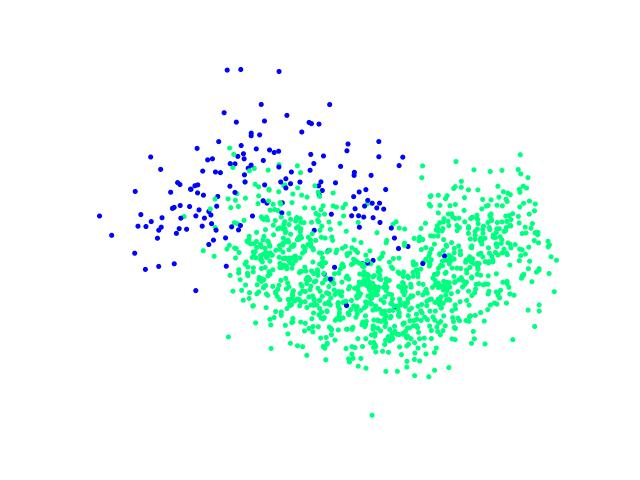
\includegraphics[width=0.9\linewidth]{Figures/moon/ImbalancedData}
	\caption{Artificial class imbalanced Moon dataset with IR of 7:1.}
	\label{fig:raw_moon}
\end{figure}


\begin{figure*}[th]
	\centering
	%[trim=left bottom right top, clip]
	\begin{subfigure}[]{0.3\linewidth}
		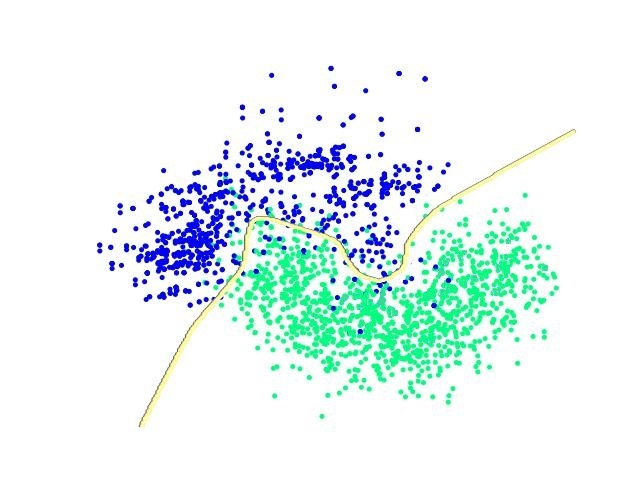
\includegraphics[width=\linewidth]{Figures/moon/Training_Data_PLot_SIMPOR}
		\caption{\Methodname{}.}
		\label{fig:simpor_moon}
	\end{subfigure}
	\hspace{0.1em}% 
	\begin{subfigure}[]{0.3\linewidth}
		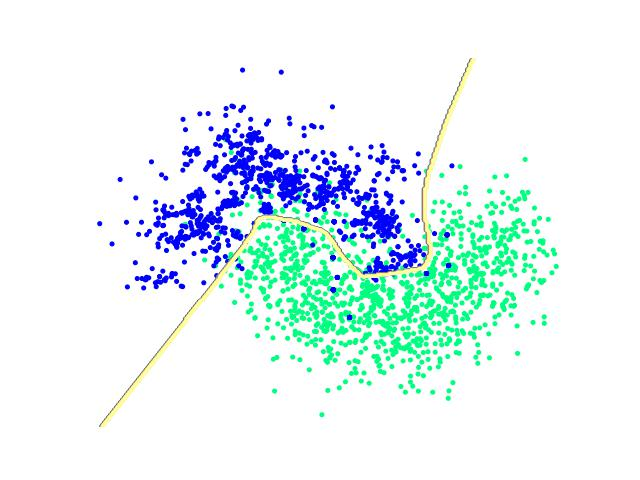
\includegraphics[width=\linewidth]{Figures/moon/Training_Data_PLot_GDO}
		\caption{GDO.}
		\label{fig:gdo_moon}
	\end{subfigure}
	\hspace{0.1em}% 
	\begin{subfigure}[]{0.3\linewidth}
		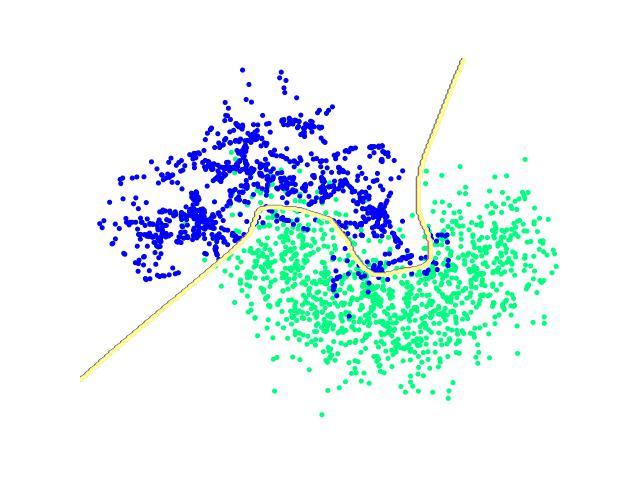
\includegraphics[width=\linewidth]{Figures/moon/Training_Data_PLot_SMOTE}
		\caption{SMOTE.}
		\label{fig:smote_moon}
	\end{subfigure}
	\\
	\begin{subfigure}[]{0.3\linewidth}
		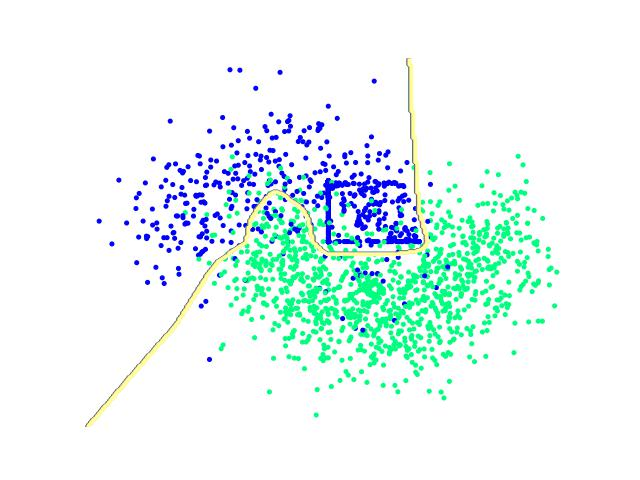
\includegraphics[width=\linewidth]{Figures/moon/Training_Data_PLot_DeepSMOTE}
		\caption{ DeepSMOTE.}
		\label{fig:deepsmote_moon}
	\end{subfigure}
	\hspace{0.1em}% 
	\begin{subfigure}[]{0.3\linewidth}
		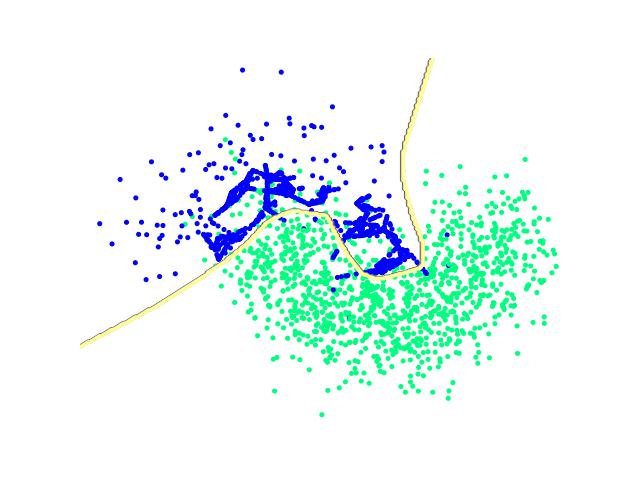
\includegraphics[width=\linewidth]{Figures/moon/Training_Data_PLot_BorderlineSMOTE}
		\caption{BorderlineSMOTE.}
		\label{fig:border_smote_moon}
	\end{subfigure}
	\hspace{0.1em}% 
	\begin{subfigure}[]{0.3\linewidth}
		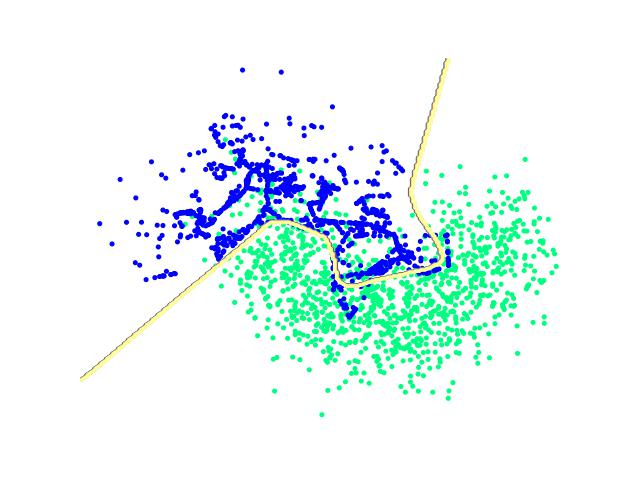
\includegraphics[width=\linewidth]{Figures/moon/Training_Data_PLot_ADASYN}
		\caption{ADASYN. }
		\label{fig:adasyn_moon}
	\end{subfigure}
	
	\caption{Data plot and model's decision boundary visualization for Moon Dataset over different techniques.}
	\label{fig:MoonResults}
\end{figure*}

\Copy{moonGeneration}{
We implement techniques on an artificial 2-dimension dataset for demonstration purposes. We first generate the balanced synthetic MOON dataset using python library \textit{sklearn.datasets.make\_moons}. The generated MOON contains 3000 samples labeled in two classes, and each instance has two numerical features with values ranging from 0 to 1. We then make the dataset artificially imbalanced with an Imbalance Ratio of 7:1 by randomly removing 1285 samples from one class.} As a result, the training dataset becomes imbalanced, as visualized in Figure \ref{fig:raw_moon}.

Figure \ref{fig:MoonResults} captures the classification for different techniques. We also visualize the model decision boundaries to provide additional information on how the classification models are affected. We use a fully connected neural network described in Table \ref{tab:model_setting} to classify the data.




% Table generated by Excel2LaTeX from sheet 'Accuracy'
\begin{table}[htbp!]
	\centering
	\caption{Classification Result on Moon Dataset.}
	\resizebox{\columnwidth}{!}{%
		
	\begin{tabular}{crcccccc}
		Metric &       & SIMPOR & SMOTE & BL-SMOTE & DeepSMOTE   & ADASYN & GDO \bigstrut[b]\\
		\hline
		F1-score &       & 0.883 & 0.824 & 0.827 & 0.842 & 0.785 & 0.817 \bigstrut[t]\\
		AUC   &       & 0.961 & 0.957 & 0.955 & 0.959 & 0.955 & 0.959 \\
	\end{tabular}%

}
	\label{tab:MoonPerformance}
\end{table}%

\subsubsection{Results and Discussion}
From the visualization shown in Figure \ref{fig:MoonResults} and the classification performance results in Table \ref{tab:MoonPerformance}, it is clear that \Methodname{} performs better than others by up to 10\% on F1-score and 1.1\% on AUC. We can see that DeepSMOTE (DeepSM) creates dense squared noise and pushes the decision boundary to the majority class. Due to the fact that SMOTE-based methods does not take the informative region into account, unbalanced data in this area lead to a severe error in decision boundary. In Figures \ref{fig:adasyn_moon} and \ref{fig:border_smote_moon}, BorderlineSMOTE (BL-SMOTE) and ADASYN focus on the area near the model's decision boundary, but they inherit a drawback from SMOTE; any noise or mislabeled samples can, unfortunately, create very dense bridges crossing the expected border and lead to decision errors. Figure \ref{fig:gdo_moon} shows that GDO also generates local gaussian groups of samples near the boder and thus create errors. This phenomenon might cause by a few mis-labeled sample points. In contrast, by generating neighbors of minority samples in the direction towards the minority class and balancing the informative region, \Methodname{} (Figure \ref{fig:simpor_moon}) helps the classifier to make a better decision with a solid smooth decision boundary. Poorly-placed synthetic samples are significantly less than that of others. 


\subsection{\Methodname{} on forty-one real datasets}
\label{subsec:41Datasets}
\Copy{datasetDetail}{
In this section, we compare the proposed technique on 41 real two-class datasets with a variable number of features and Imbalance Ratios, i.e., KEEL datasets \cite{ KEEL_detail,KEEL_dataset}, UCI datasets fetched from Sklearn tool \cite{imbalancedlearnFetch_datasetsx2014, uci_imbalance_dataset} and Credit Card Fraud \cite{kaggleCreditCard} dataset. Since the original Credit Card Fraud contains a large number of banking normal and fraud transaction samples (284,807) which significantly reduces our experimental efficiency, we reduced the dataset size by randomly removing normal class transactions to reach an imbalance ratio of 3.0. Other datasets are kept as their original versions after removing bad samples (containing Null values). The datasets are described in Table \ref{tab:dataDecription}. 
}
\subsubsection{Classification results}
\label{sec:classificationResult}
% Table generated by Excel2LaTeX from sheet 'MacroF1'

\begin{table}[!htbp]
	\centering
	\caption{F1-score over different datasets.}
	\resizebox{0.97\columnwidth}{!}{%
	
  \begin{tabular}{lrrrrrrrr}
  	\toprule
  	& \multicolumn{1}{c}{SIMPOR} & \multicolumn{1}{c}{GDO} & \multicolumn{1}{c}{SMOTE} & \multicolumn{1}{c}{BL-SMOTE} & \multicolumn{1}{c}{ADASYN} & \multicolumn{1}{c}{DeepSM} & \multicolumn{1}{c}{SVMCS} & \multicolumn{1}{c}{EE} \\
  	\midrule
  	glass1 & 0.729 & \textbf{0.741} & 0.707 & 0.729 & 0.729 & 0.706 & 0.719 & 0.705 \\
  	wisconsin & \textbf{0.962} & 0.959 & 0.953 & 0.958 & 0.956 & 0.960 & 0.958 & 0.957 \\
  	pima  & \textbf{0.777} & 0.699 & 0.714 & 0.720 & 0.700 & 0.721 & 0.742 & 0.731 \\
  	glass0 & \textbf{0.840} & 0.799 & 0.804 & 0.795 & 0.806 & 0.813 & 0.835 & 0.811 \\
  	yeast1 & \textbf{0.715} & 0.676 & 0.675 & 0.685 & 0.672 & 0.673 & 0.685 & 0.678 \\
  	haberman & \textbf{0.601} & 0.599 & 0.589 & 0.587 & 0.580 & 0.587 & 0.586 & 0.584 \\
  	vehicle1 & \textbf{0.824} & 0.815 & 0.807 & 0.796 & 0.817 & 0.785 & 0.784 & 0.808 \\
  	vehicle2 & \textbf{0.987} & 0.967 & 0.977 & 0.978 & 0.981 & 0.954 & 0.976 & 0.981 \\
  	vehicle3 & \textbf{0.821} & 0.766 & 0.785 & 0.792 & 0.806 & 0.780 & 0.782 & 0.785 \\
  	creditcard & \textbf{0.954} & 0.935 & 0.946 & 0.944 & 0.943 & 0.947 & 0.907 & 0.939 \\
  	glass-0-1-2-3\_vs\_4-5-6 & 0.850 & 0.923 & 0.918 & 0.912 & 0.915 & \textbf{0.929} & 0.907 & 0.905 \\
  	vehicle0 & 0.933 & 0.956 & \textbf{0.970} & 0.965 & 0.965 & 0.952 & \textbf{0.970} & 0.969 \\
  	ecoli1 & 0.831 & 0.822 & 0.838 & 0.818 & 0.815 & \textbf{0.853} & 0.824 & 0.827 \\
  	new-thyroid1 & 0.970 & \textbf{0.979} & 0.946 & 0.953 & 0.953 & 0.902 & 0.946 & 0.946 \\
  	new-thyroid2 & 0.962 & \textbf{0.982} & 0.938 & 0.938 & 0.938 & 0.872 & 0.930 & 0.930 \\
  	ecoli2 & \textbf{0.922} & 0.880 & 0.905 & 0.864 & 0.884 & 0.887 & 0.909 & 0.914 \\
  	glass6 & \textbf{0.952} & 0.899 & 0.875 & 0.880 & 0.869 & 0.864 & 0.880 & 0.880 \\
  	yeast3 & 0.862 & 0.818 & 0.842 & 0.836 & 0.829 & 0.831 & 0.867 & \textbf{0.879} \\
  	ecoli3 & 0.806 & 0.791 & 0.790 & 0.792 & 0.792 & \textbf{0.829} & 0.827 & 0.824 \\
  	page-blocks0 & \textbf{0.926} & 0.904 & 0.909 & 0.900 & 0.900 & 0.913 & 0.919 & 0.912 \\
  	yeast-2\_vs\_4 & 0.883 & 0.875 & \textbf{0.893} & 0.844 & 0.866 & 0.817 & 0.807 & 0.772 \\
  	yeast-0-5-6-7-9\_vs\_4 & \textbf{0.824} & 0.752 & 0.754 & 0.781 & 0.758 & 0.747 & 0.813 & 0.805 \\
  	vowel0 & \textbf{1.000} & \textbf{1.000} & \textbf{1.000} & \textbf{1.000} & \textbf{1.000} & 0.997 & \textbf{1.000} & 0.997 \\
  	glass-0-1-6\_vs\_2 & \textbf{0.771} & 0.692 & 0.733 & 0.725 & 0.707 & 0.524 & 0.685 & 0.646 \\
  	glass2 & 0.737 & 0.717 & \textbf{0.839} & 0.805 & 0.801 & 0.779 & 0.701 & 0.666 \\
  	yeast-1\_vs\_7 & \textbf{0.710} & 0.663 & 0.595 & 0.654 & 0.608 & 0.614 & 0.681 & 0.691 \\
  	glass4 & 0.795 & 0.871 & 0.846 & 0.850 & 0.859 & \textbf{0.892} & 0.811 & 0.819 \\
  	ecoli4 & \textbf{0.909} & 0.841 & 0.893 & 0.883 & 0.883 & 0.863 & 0.893 & 0.893 \\
  	page-blocks-1-3\_vs\_4 & 0.982 & 0.944 & 0.964 & 0.972 & 0.964 & 0.982 & \textbf{0.990} & \textbf{0.990} \\
  	abalone9-18 & 0.777 & 0.763 & 0.760 & 0.767 & 0.773 & 0.752 & \textbf{0.817} & 0.792 \\
  	yeast-1-4-5-8\_vs\_7 & 0.593 & \textbf{0.637} & 0.584 & 0.618 & 0.628 & 0.487 & 0.489 & 0.489 \\
  	glass5 & 0.912 & 0.843 & 0.792 & \textbf{0.919} & 0.780 & 0.792 & 0.633 & 0.633 \\
  	yeast-2\_vs\_8 & \textbf{0.884} & 0.758 & 0.746 & 0.772 & 0.750 & 0.823 & 0.876 & 0.876 \\
  	car\_eval\_4 & \textbf{1.000} & 0.967 & 0.997 & 0.994 & 0.997 & 0.993 & \textbf{1.000} & \textbf{1.000} \\
  	wine\_quality & \textbf{0.753} & 0.681 & 0.660 & 0.690 & 0.674 & 0.669 & 0.675 & 0.674 \\
  	yeast\_me2 & 0.701 & 0.638 & 0.668 & 0.655 & 0.656 & 0.690 & \textbf{0.707} & 0.702 \\
  	yeast4 & \textbf{0.793} & 0.698 & 0.682 & 0.690 & 0.671 & 0.738 & 0.752 & 0.752 \\
  	yeast-1-2-8-9\_vs\_7 & \textbf{0.775} & 0.642 & 0.612 & 0.633 & 0.607 & 0.698 & 0.750 & 0.750 \\
  	yeast5 & 0.667 & 0.854 & 0.871 & 0.877 & \textbf{0.881} & 0.786 & 0.839 & 0.844 \\
  	yeast6 & \textbf{0.745} & 0.734 & 0.730 & 0.724 & 0.705 & 0.696 & 0.708 & 0.738 \\
  	abalone19 & 0.498 & 0.500 & \textbf{0.526} & 0.518 & 0.524 & 0.497 & 0.498 & 0.498 \\
  	\bottomrule
  \end{tabular}%
	}
	\label{tab:F1AllDatasets}%
\end{table}%

% Table generated by Excel2LaTeX from sheet 'MicroGmean'
\begin{table}[!htbp]
	\centering
	\caption{AUC result over different datasets.}
	\resizebox{0.97\columnwidth}{!}{%
		
     \begin{tabular}{lrrrrrrrr}
 	\toprule
 	& \multicolumn{1}{c}{SIMPOR} & \multicolumn{1}{c}{GDO} & \multicolumn{1}{c}{SMOTE} & \multicolumn{1}{c}{BL-SMOTE} & \multicolumn{1}{c}{ADASYN} & \multicolumn{1}{c}{DeepSM} & \multicolumn{1}{c}{SVMCS} & \multicolumn{1}{c}{EE} \\
 	\midrule
 	glass1 & 0.798 & \textbf{0.818} & 0.788 & 0.782 & 0.807 & 0.804 & 0.800 & 0.795 \\
 	wisconsin & \textbf{0.995} & 0.992 & 0.992 & 0.992 & 0.992 & 0.991 & \textbf{0.995} & 0.994 \\
 	pima  & \textbf{0.858} & 0.790 & 0.800 & 0.804 & 0.782 & 0.810 & 0.826 & 0.818 \\
 	glass0 & \textbf{0.901} & 0.879 & 0.885 & 0.859 & 0.873 & 0.891 & 0.896 & 0.882 \\
 	yeast1 & \textbf{0.811} & 0.758 & 0.753 & 0.753 & 0.746 & 0.776 & 0.782 & 0.774 \\
 	haberman & 0.675 & 0.662 & 0.660 & 0.673 & 0.667 & 0.686 & 0.686 & \textbf{0.689} \\
 	vehicle1 & \textbf{0.936} & 0.917 & 0.922 & 0.920 & 0.929 & 0.924 & 0.920 & 0.928 \\
 	vehicle2 & \textbf{0.999} & 0.998 & \textbf{0.999} & \textbf{0.999} & \textbf{0.999} & 0.991 & \textbf{0.999} & \textbf{0.999} \\
 	vehicle3 & \textbf{0.918} & 0.871 & 0.895 & 0.897 & 0.900 & 0.901 & 0.903 & 0.904 \\
 	creditcard & \textbf{0.974} & 0.969 & 0.966 & 0.962 & 0.962 & 0.961 & 0.968 & 0.945 \\
 	glass-0-1-2-3\_vs\_4-5-6 & 0.968 & 0.987 & \textbf{0.989} & 0.976 & 0.988 & 0.987 & 0.985 & 0.985 \\
 	vehicle0 & 0.975 & 0.991 & 0.995 & 0.995 & \textbf{0.996} & 0.992 & 0.995 & \textbf{0.996} \\
 	ecoli1 & 0.949 & 0.948 & \textbf{0.952} & 0.942 & 0.943 & 0.951 & 0.951 & 0.950 \\
 	new-thyroid1 & \textbf{0.999} & \textbf{0.999} & 0.997 & 0.997 & 0.997 & 0.982 & 0.997 & 0.997 \\
 	new-thyroid2 & \textbf{0.999} & \textbf{0.999} & 0.998 & 0.998 & 0.997 & 0.977 & 0.998 & \textbf{0.999} \\
 	ecoli2 & 0.950 & 0.953 & 0.957 & 0.946 & 0.958 & 0.957 & 0.959 & \textbf{0.960} \\
 	glass6 & \textbf{0.963} & 0.960 & 0.920 & 0.833 & 0.841 & 0.894 & 0.939 & 0.877 \\
 	yeast3 & \textbf{0.968} & 0.943 & 0.935 & 0.927 & 0.937 & 0.946 & 0.966 & 0.967 \\
 	ecoli3 & 0.883 & 0.879 & 0.878 & 0.880 & 0.883 & 0.891 & \textbf{0.897} & 0.885 \\
 	page-blocks0 & \textbf{0.990} & 0.986 & 0.969 & 0.982 & 0.984 & 0.981 & 0.986 & 0.986 \\
 	yeast-2\_vs\_4 & 0.974 & \textbf{0.976} & 0.961 & 0.959 & 0.960 & 0.907 & 0.972 & 0.949 \\
 	yeast-0-5-6-7-9\_vs\_4 & 0.915 & \textbf{0.923} & 0.881 & 0.904 & 0.866 & 0.876 & 0.918 & 0.914 \\
 	vowel0 & \textbf{1.000} & \textbf{1.000} & \textbf{1.000} & \textbf{1.000} & \textbf{1.000} & \textbf{1.000} & \textbf{1.000} & \textbf{1.000} \\
 	glass-0-1-6\_vs\_2 & \textbf{0.942} & 0.897 & 0.905 & 0.892 & 0.910 & 0.886 & 0.907 & 0.941 \\
 	glass2 & 0.929 & 0.917 & 0.923 & 0.923 & \textbf{0.952} & 0.919 & 0.940 & 0.932 \\
 	yeast-1\_vs\_7 & \textbf{0.848} & 0.777 & 0.677 & 0.761 & 0.685 & 0.702 & 0.791 & 0.795 \\
 	glass4 & 0.955 & 0.976 & 0.954 & \textbf{0.987} & 0.949 & 0.979 & 0.972 & 0.975 \\
 	ecoli4 & \textbf{0.997} & 0.978 & 0.984 & 0.984 & 0.989 & 0.953 & 0.990 & 0.988 \\
 	page-blocks-1-3\_vs\_4 & \textbf{1.000} & 0.997 & 0.999 & 0.999 & 0.999 & 0.999 & 0.999 & 0.999 \\
 	abalone9-18 & 0.934 & 0.920 & 0.933 & 0.929 & 0.919 & 0.898 & 0.930 & \textbf{0.940} \\
 	yeast-1-4-5-8\_vs\_7 & \textbf{0.823} & 0.746 & 0.721 & 0.734 & 0.721 & 0.721 & 0.769 & 0.754 \\
 	glass5 & 0.987 & \textbf{0.990} & 0.985 & 0.983 & 0.987 & 0.987 & \textbf{0.990} & 0.988 \\
 	yeast-2\_vs\_8 & 0.855 & 0.845 & 0.835 & \textbf{0.865} & 0.853 & 0.802 & 0.809 & 0.805 \\
 	car\_eval\_4 & \textbf{1.000} & \textbf{1.000} & \textbf{1.000} & \textbf{1.000} & \textbf{1.000} & \textbf{1.000} & \textbf{1.000} & \textbf{1.000} \\
 	wine\_quality & \textbf{0.852} & 0.783 & 0.727 & 0.756 & 0.740 & 0.793 & 0.781 & 0.805 \\
 	yeast\_me2 & \textbf{0.896} & 0.887 & 0.793 & 0.817 & 0.787 & 0.832 & 0.871 & 0.874 \\
 	yeast4 & \textbf{0.935} & 0.889 & 0.796 & 0.810 & 0.792 & 0.817 & 0.832 & 0.848 \\
 	yeast-1-2-8-9\_vs\_7 & \textbf{0.761} & 0.699 & 0.702 & 0.687 & 0.685 & 0.695 & 0.745 & 0.756 \\
 	yeast5 & 0.835 & 0.991 & 0.985 & 0.984 & 0.985 & 0.983 & 0.992 & \textbf{0.993} \\
 	yeast6 & 0.960 & 0.936 & 0.905 & 0.946 & 0.906 & 0.933 & 0.959 & \textbf{0.963} \\
 	abalone19 & \textbf{0.782} & 0.557 & 0.616 & 0.676 & 0.575 & 0.721 & 0.763 & 0.771 \\
 	\bottomrule
 \end{tabular}%
		
	}
	\label{tab:AUCAllDatasets}%
\end{table}%


\Copy{precisionAndRecall}{
\begin{table}[hbp]
	\centering
	\caption{Precision results over 41 datasets.}
	\resizebox{0.97\columnwidth}{!}{%
		
 \begin{tabular}{lrrrrrrrr}
	\toprule
	& \multicolumn{1}{c}{SIMPOR} & \multicolumn{1}{c}{GDO} & \multicolumn{1}{c}{SMOTE} & \multicolumn{1}{c}{BL-SMOTE} & \multicolumn{1}{c}{ADASYN} & \multicolumn{1}{c}{DeepSM} & \multicolumn{1}{c}{SVMCS} & \multicolumn{1}{c}{EE} \\
	\midrule
	glass1 & 0.733 & \textbf{0.744} & 0.710 & 0.732 & 0.730 & 0.710 & 0.726 & 0.711 \\
	wisconsin & \textbf{0.959} & 0.955 & 0.952 & 0.956 & 0.954 & 0.957 & 0.956 & 0.955 \\
	pima  & \textbf{0.776} & 0.694 & 0.714 & 0.715 & 0.700 & 0.727 & 0.752 & 0.737 \\
	glass0 & \textbf{0.836} & 0.782 & 0.796 & 0.782 & 0.795 & 0.809 & 0.825 & 0.808 \\
	yeast1 & \textbf{0.727} & 0.674 & 0.670 & 0.680 & 0.668 & 0.687 & 0.702 & 0.689 \\
	haberman & \textbf{0.610} & 0.588 & 0.578 & 0.574 & 0.570 & 0.592 & 0.603 & 0.608 \\
	vehicle1 & \textbf{0.835} & 0.803 & 0.811 & 0.804 & 0.819 & 0.797 & 0.793 & 0.817 \\
	vehicle2 & \textbf{0.986} & 0.954 & 0.970 & 0.973 & 0.977 & 0.944 & 0.971 & 0.977 \\
	vehicle3 & \textbf{0.826} & 0.760 & 0.779 & 0.797 & 0.807 & 0.788 & 0.794 & 0.798 \\
	creditcard & \textbf{0.961} & 0.933 & 0.955 & 0.953 & 0.951 & 0.958 & 0.904 & 0.954 \\
	glass-0-1-2-3\_vs\_4-5-6 & 0.845 & 0.915 & 0.922 & 0.915 & 0.911 & \textbf{0.925} & 0.907 & 0.911 \\
	vehicle0 & 0.921 & 0.935 & 0.960 & 0.960 & 0.956 & 0.959 & \textbf{0.971} & 0.969 \\
	ecoli1 & 0.810 & 0.795 & 0.811 & 0.792 & 0.784 & \textbf{0.827} & 0.813 & 0.816 \\
	new-thyroid1 & \textbf{0.977} & 0.964 & 0.950 & 0.953 & 0.953 & 0.903 & 0.950 & 0.950 \\
	new-thyroid2 & \textbf{0.974} & 0.971 & 0.966 & 0.966 & 0.966 & 0.886 & 0.963 & 0.963 \\
	ecoli2 & \textbf{0.928} & 0.849 & 0.901 & 0.852 & 0.867 & 0.867 & 0.915 & 0.924 \\
	glass6 & 0.977 & 0.922 & 0.941 & \textbf{0.980} & 0.926 & 0.920 & \textbf{0.980} & \textbf{0.980} \\
	yeast3 & 0.868 & 0.777 & 0.825 & 0.815 & 0.786 & 0.829 & 0.867 & \textbf{0.876} \\
	ecoli3 & 0.791 & 0.726 & 0.739 & 0.743 & 0.734 & 0.806 & \textbf{0.842} & 0.838 \\
	page-blocks0 & 0.929 & 0.858 & 0.897 & 0.870 & 0.854 & \textbf{0.936} & 0.922 & 0.913 \\
	yeast-2\_vs\_4 & 0.874 & 0.846 & \textbf{0.907} & 0.864 & 0.865 & 0.830 & 0.750 & 0.818 \\
	yeast-0-5-6-7-9\_vs\_4 & 0.835 & 0.688 & 0.741 & 0.755 & 0.721 & 0.748 & 0.861 & \textbf{0.868} \\
	vowel0 & \textbf{1.000} & \textbf{1.000} & \textbf{1.000} & \textbf{1.000} & \textbf{1.000} & 0.999 & \textbf{1.000} & 0.999 \\
	glass-0-1-6\_vs\_2 & \textbf{0.822} & 0.710 & 0.760 & 0.728 & 0.720 & 0.531 & 0.664 & 0.619 \\
	glass2 & 0.731 & 0.653 & \textbf{0.765} & 0.764 & 0.723 & 0.758 & 0.739 & 0.649 \\
	yeast-1\_vs\_7 & \textbf{0.779} & 0.613 & 0.580 & 0.632 & 0.584 & 0.693 & 0.740 & 0.759 \\
	glass4 & 0.756 & 0.845 & 0.910 & 0.927 & 0.853 & \textbf{0.985} & 0.887 & 0.899 \\
	ecoli4 & \textbf{0.896} & 0.792 & 0.879 & 0.862 & 0.862 & 0.808 & 0.879 & 0.879 \\
	page-blocks-1-3\_vs\_4 & 0.967 & 0.903 & 0.935 & 0.949 & 0.935 & 0.969 & \textbf{0.982} & \textbf{0.982} \\
	abalone9-18 & 0.806 & 0.706 & 0.717 & 0.731 & 0.731 & 0.762 & \textbf{0.903} & 0.866 \\
	yeast-1-4-5-8\_vs\_7 & \textbf{0.668} & 0.574 & 0.557 & 0.582 & 0.579 & 0.479 & 0.479 & 0.479 \\
	glass5 & 0.912 & 0.823 & 0.824 & \textbf{0.954} & 0.803 & 0.824 & 0.673 & 0.673 \\
	yeast-2\_vs\_8 & 0.913 & 0.728 & 0.670 & 0.752 & 0.682 & 0.825 & \textbf{0.921} & \textbf{0.921} \\
	car\_eval\_4 & \textbf{1.000} & 0.939 & 0.994 & 0.988 & 0.994 & 0.999 & \textbf{1.000} & \textbf{1.000} \\
	wine\_quality & \textbf{0.758} & 0.659 & 0.682 & 0.713 & 0.682 & 0.727 & 0.723 & 0.736 \\
	yeast\_me2 & 0.737 & 0.593 & 0.666 & 0.652 & 0.641 & 0.738 & \textbf{0.852} & 0.843 \\
	yeast4 & 0.800 & 0.635 & 0.640 & 0.660 & 0.629 & 0.738 & 0.829 & \textbf{0.831} \\
	yeast-1-2-8-9\_vs\_7 & 0.909 & 0.598 & 0.587 & 0.620 & 0.589 & 0.842 & 0.957 & \textbf{0.988} \\
	yeast5 & 0.629 & 0.759 & 0.804 & 0.807 & \textbf{0.821} & 0.753 & 0.807 & 0.816 \\
	yeast6 & 0.785 & 0.662 & 0.671 & 0.729 & 0.657 & 0.714 & 0.740 & \textbf{0.801} \\
	abalone19 & 0.497 & 0.498 & 0.516 & \textbf{0.517} & 0.511 & 0.497 & 0.497 & 0.497 \\
	\bottomrule
\end{tabular}%
		
	}
	\label{tab:Precision}%
\end{table}%


\begin{table}[htbp]
	\centering
	\caption{Recall results over 41 datasets.}
	\resizebox{0.97\columnwidth}{!}{%
	       \begin{tabular}{lrrrrrrrr}
	       	\toprule
	       	& \multicolumn{1}{c}{SIMPOR} & \multicolumn{1}{c}{GDO} & \multicolumn{1}{c}{SMOTE} & \multicolumn{1}{c}{BL-SMOTE} & \multicolumn{1}{c}{ADASYN} & \multicolumn{1}{c}{DeepSM} & \multicolumn{1}{c}{SVMCS} & \multicolumn{1}{c}{EE} \\
	       	\midrule
	       	glass1 & 0.725 & \textbf{0.739} & 0.705 & 0.726 & 0.727 & 0.702 & 0.713 & 0.699 \\
	       	wisconsin & \textbf{0.965} & 0.963 & 0.955 & 0.961 & 0.959 & 0.962 & 0.960 & 0.958 \\
	       	pima  & \textbf{0.778} & 0.705 & 0.714 & 0.727 & 0.701 & 0.715 & 0.733 & 0.726 \\
	       	glass0 & 0.844 & 0.817 & 0.814 & 0.810 & 0.818 & 0.817 & \textbf{0.847} & 0.815 \\
	       	yeast1 & \textbf{0.704} & 0.679 & 0.680 & 0.691 & 0.677 & 0.660 & 0.669 & 0.668 \\
	       	haberman & 0.593 & \textbf{0.611} & 0.601 & 0.599 & 0.590 & 0.583 & 0.570 & 0.563 \\
	       	vehicle1 & 0.814 & \textbf{0.827} & 0.803 & 0.789 & 0.816 & 0.774 & 0.777 & 0.800 \\
	       	vehicle2 & \textbf{0.988} & 0.980 & 0.983 & 0.983 & 0.985 & 0.965 & 0.982 & 0.986 \\
	       	vehicle3 & \textbf{0.817} & 0.772 & 0.791 & 0.787 & 0.806 & 0.772 & 0.770 & 0.773 \\
	       	creditcard & \textbf{0.948} & 0.937 & 0.937 & 0.936 & 0.935 & 0.936 & 0.911 & 0.925 \\
	       	glass-0-1-2-3\_vs\_4-5-6 & 0.857 & 0.932 & 0.915 & 0.910 & 0.920 & \textbf{0.935} & 0.909 & 0.901 \\
	       	vehicle0 & 0.947 & \textbf{0.979} & \textbf{0.979} & 0.971 & 0.973 & 0.946 & 0.969 & 0.969 \\
	       	ecoli1 & 0.854 & 0.852 & 0.866 & 0.847 & 0.849 & \textbf{0.880} & 0.837 & 0.839 \\
	       	new-thyroid1 & 0.965 & \textbf{0.995} & 0.942 & 0.953 & 0.953 & 0.901 & 0.942 & 0.942 \\
	       	new-thyroid2 & 0.951 & \textbf{0.995} & 0.913 & 0.913 & 0.913 & 0.859 & 0.900 & 0.900 \\
	       	ecoli2 & \textbf{0.916} & 0.913 & 0.911 & 0.878 & 0.902 & 0.910 & 0.903 & 0.905 \\
	       	glass6 & \textbf{0.931} & 0.880 & 0.818 & 0.800 & 0.820 & 0.816 & 0.800 & 0.800 \\
	       	yeast3 & 0.856 & 0.863 & 0.862 & 0.860 & 0.878 & 0.834 & 0.869 & \textbf{0.883} \\
	       	ecoli3 & 0.823 & \textbf{0.870} & 0.850 & 0.850 & 0.861 & 0.855 & 0.816 & 0.814 \\
	       	page-blocks0 & 0.923 & \textbf{0.955} & 0.924 & 0.932 & 0.952 & 0.892 & 0.917 & 0.913 \\
	       	yeast-2\_vs\_4 & 0.895 & \textbf{0.908} & 0.881 & 0.827 & 0.868 & 0.810 & 0.875 & 0.741 \\
	       	yeast-0-5-6-7-9\_vs\_4 & 0.814 & \textbf{0.832} & 0.770 & 0.815 & 0.802 & 0.771 & 0.772 & 0.752 \\
	       	vowel0 & \textbf{1.000} & \textbf{1.000} & \textbf{1.000} & \textbf{1.000} & \textbf{1.000} & 0.995 & \textbf{1.000} & 0.995 \\
	       	glass-0-1-6\_vs\_2 & \textbf{0.741} & 0.680 & 0.735 & 0.735 & 0.730 & 0.520 & 0.716 & 0.682 \\
	       	glass2 & 0.747 & 0.800 & \textbf{0.939} & 0.869 & 0.907 & 0.812 & 0.677 & 0.689 \\
	       	yeast-1\_vs\_7 & 0.655 & \textbf{0.722} & 0.611 & 0.678 & 0.634 & 0.562 & 0.633 & 0.635 \\
	       	glass4 & 0.841 & \textbf{0.906} & 0.795 & 0.795 & 0.872 & 0.821 & 0.759 & 0.761 \\
	       	ecoli4 & \textbf{0.934} & 0.901 & 0.911 & 0.909 & 0.909 & 0.928 & 0.911 & 0.911 \\
	       	page-blocks-1-3\_vs\_4 & 0.998 & 0.992 & 0.996 & 0.997 & 0.996 & 0.998 & \textbf{0.999} & \textbf{0.999} \\
	       	abalone9-18 & 0.751 & \textbf{0.830} & 0.812 & 0.812 & 0.823 & 0.748 & 0.751 & 0.733 \\
	       	yeast-1-4-5-8\_vs\_7 & 0.549 & \textbf{0.723} & 0.618 & 0.665 & 0.697 & 0.495 & 0.499 & 0.499 \\
	       	glass5 & \textbf{0.912} & 0.868 & 0.768 & 0.893 & 0.766 & 0.768 & 0.602 & 0.602 \\
	       	yeast-2\_vs\_8 & \textbf{0.872} & 0.835 & 0.858 & 0.838 & 0.858 & 0.845 & 0.848 & 0.848 \\
	       	car\_eval\_4 & \textbf{1.000} & 0.997 & \textbf{1.000} & 0.999 & \textbf{1.000} & 0.986 & \textbf{1.000} & \textbf{1.000} \\
	       	wine\_quality & \textbf{0.750} & 0.706 & 0.639 & 0.670 & 0.667 & 0.620 & 0.634 & 0.623 \\
	       	yeast\_me2 & 0.671 & \textbf{0.693} & 0.670 & 0.658 & 0.673 & 0.647 & 0.610 & 0.609 \\
	       	yeast4 & \textbf{0.790} & 0.776 & 0.732 & 0.725 & 0.722 & 0.741 & 0.690 & 0.690 \\
	       	yeast-1-2-8-9\_vs\_7 & 0.685 & \textbf{0.694} & 0.641 & 0.649 & 0.627 & 0.602 & 0.622 & 0.604 \\
	       	yeast5 & 0.716 & \textbf{0.979} & 0.955 & 0.964 & 0.956 & 0.830 & 0.883 & 0.883 \\
	       	yeast6 & 0.714 & \textbf{0.827} & 0.813 & 0.723 & 0.776 & 0.691 & 0.681 & 0.691 \\
	       	abalone19 & 0.499 & 0.503 & 0.537 & 0.518 & \textbf{0.539} & 0.497 & 0.500 & 0.500 \\
	       	\bottomrule
	       \end{tabular}%
		
	}
	\label{tab:Recall}%
\end{table}%
}

\begin{figure}[h!]
	\centering
	%[trim=left bottom right top, clip]
	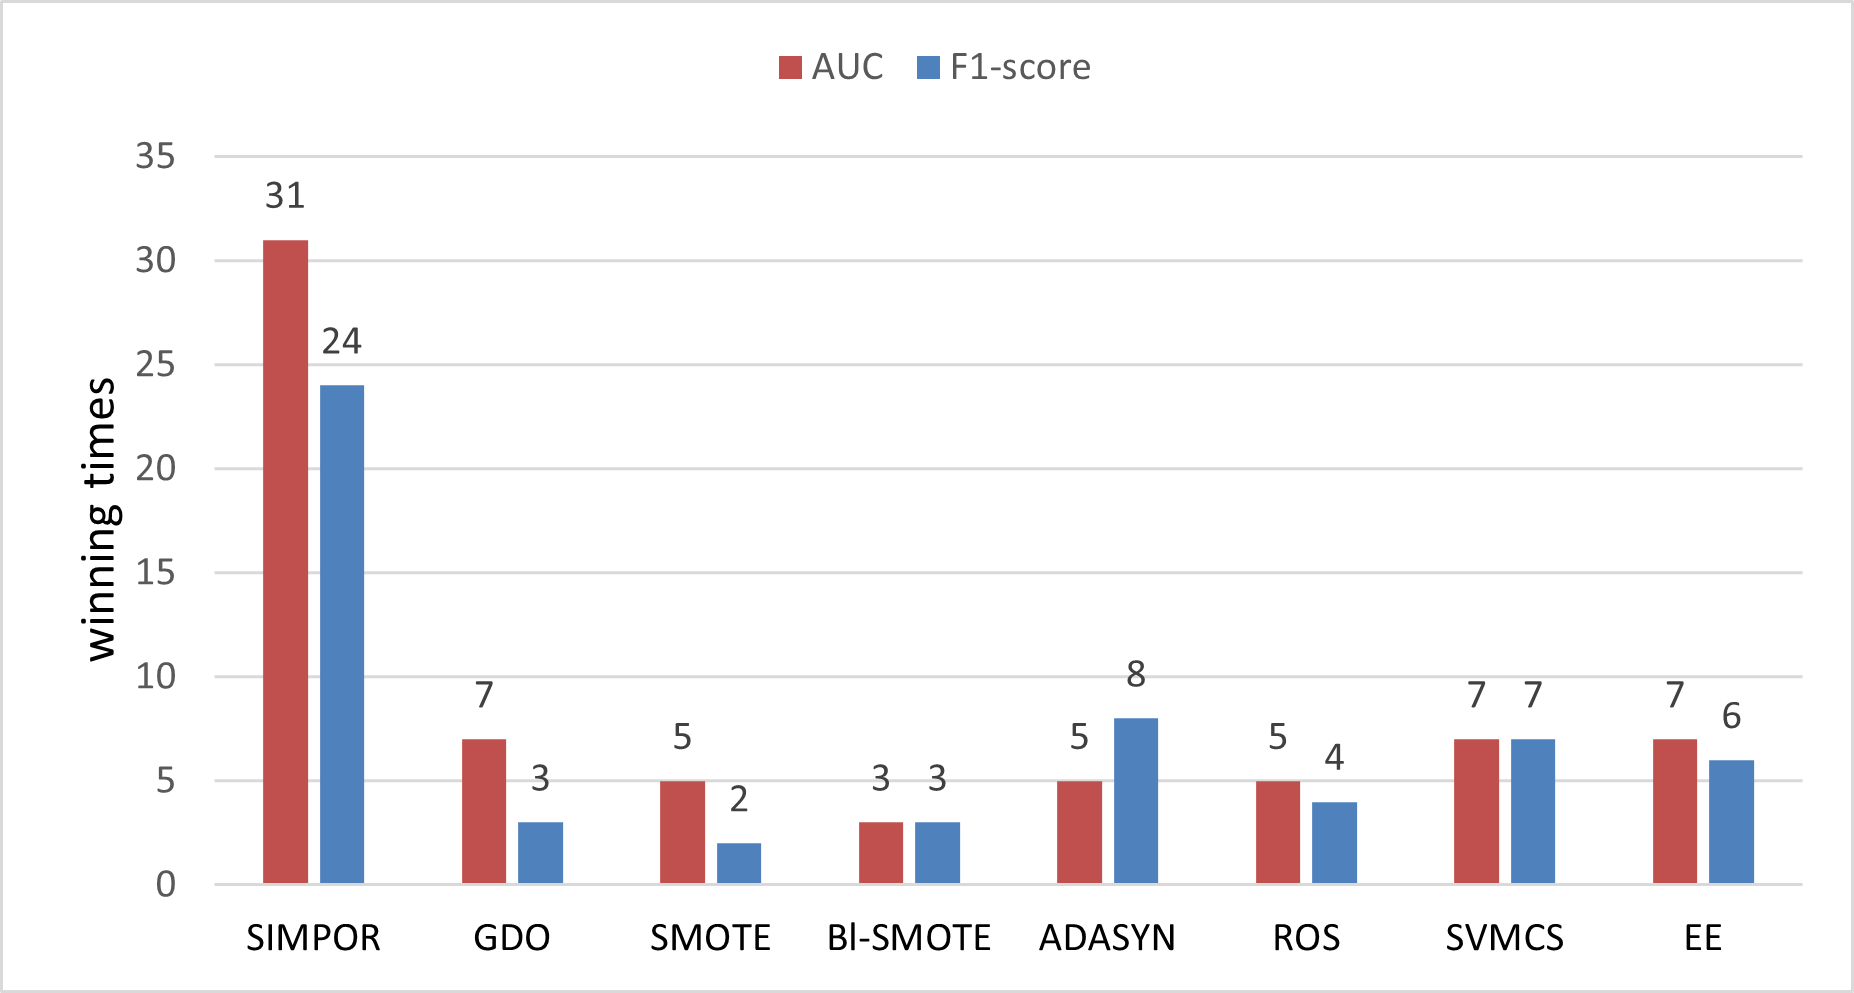
\includegraphics[width=\linewidth ]{Figures/winning_times}
	\caption{Winning times over 41 datasets.}
	\label{fig:winingTimes}
\end{figure}

Table \ref{tab:F1AllDatasets}, \ref{tab:AUCAllDatasets}, \ref{tab:Precision} and \ref{tab:Recall} show the classification F1-score, AUC, Precision, and Recall results, respectively. The highest scores for each dataset are highlighted in bold style. 
\Copy{winningTime}{We also provide the summary of the F1 and AUC scores by ``winning times" scores. We count the number of datasets for which a technique achieves the highest scores among the compared techniques and name this number ``winning times". For convention, if more than two techniques share the same highest score, the winning times will be increased for each technique. Figure \ref{fig:winingTimes} shows a summary of winning times.} 

As we can see from the table, the proposed technique outperforms others on both evaluation metrics, F1-score and AUC. More specifically, \Methodname{} hits 23 F1-score winning times and 25 AUC winning times. Its number of F1-score winning times at 23 four times better than the second winner (SVMCS) at 6, and its AUC winning times at 25 doubles the second AUC winners (EE) at 10. 


\subsection{Statistical Test.}
	\label{sec:wilcoxon}
\Copy{wilcoxonTest}{
To further evaluate the effectiveness of the technique, we also performed a Wilcoxon Signed Rank Test \cite{wilcoxon} on the 41 dataset results (F1 score and AUC). Wilcoxon hypothesis test is relevant to our study as it is a non-parametric statistical test and does not require a specific distribution assumption for the results. On the other hand, 41 data points (corresponding to 41 datasets results) are sufficient to support this test. Our null hypothesis is that the difference between the proposed technique results and those of the other technique is insignificant. Wilcoxon signed-rank test outputs are computed over the 41 dataset results and return a p-value for each technique pair. We then compare the p-value with the significant value $\alpha = 0.05$. Suppose the p-value is smaller than $\alpha$. In that case, the evidence is sufficient to reject the hypothesis, which means the proposed technique does make a significant difference from the others, and vice versa. Table \ref{tab:wilcoxonTest} shows the Wilcoxon p-value results.

	\begin{table}[htbp]
		\centering
		\caption{Wilcoxon Signed Rank Hypothesis Test results.}
		
		\begin{tabular}{lcc}
			\toprule
			& \multicolumn{2}{c}{p-value} \\
			\midrule
			SIMPOR vs. & \multicolumn{1}{l|}{F1-score} & \multicolumn{1}{l}{AUC} \\
			\midrule
			GDO   & 1.82E-03 & 1.93E-03 \\
			SMOTE & 2.66E-03 & 6.64E-05 \\
			BL\_SMOTE & 4.22E-03 & 1.63E-04 \\
			ADASYN & 2.89E-03 & 6.13E-04 \\
			DeepSM   & 6.40E-04 & 2.57E-04 \\
			SVMCS & 2.74E-03 & 3.40E-02 \\
			EE    & 1.99E-03 & 2.17E-02 \\
			\bottomrule
		\end{tabular}%
		\label{tab:wilcoxonTest}%
	\end{table}%

As we can see from Table \ref{tab:wilcoxonTest}, the p-values are all smaller than the critical value of 0.05. Thus, the null hypothesis can be rejected as the supporting evidence is sufficient. In other words, the statistical result shows that the proposed technique makes a significant improvement compared to others.     
}


\subsection{Data visualization}  

\begin{figure*}[h!]
	\centering
	%[trim=left bottom right top, clip]
	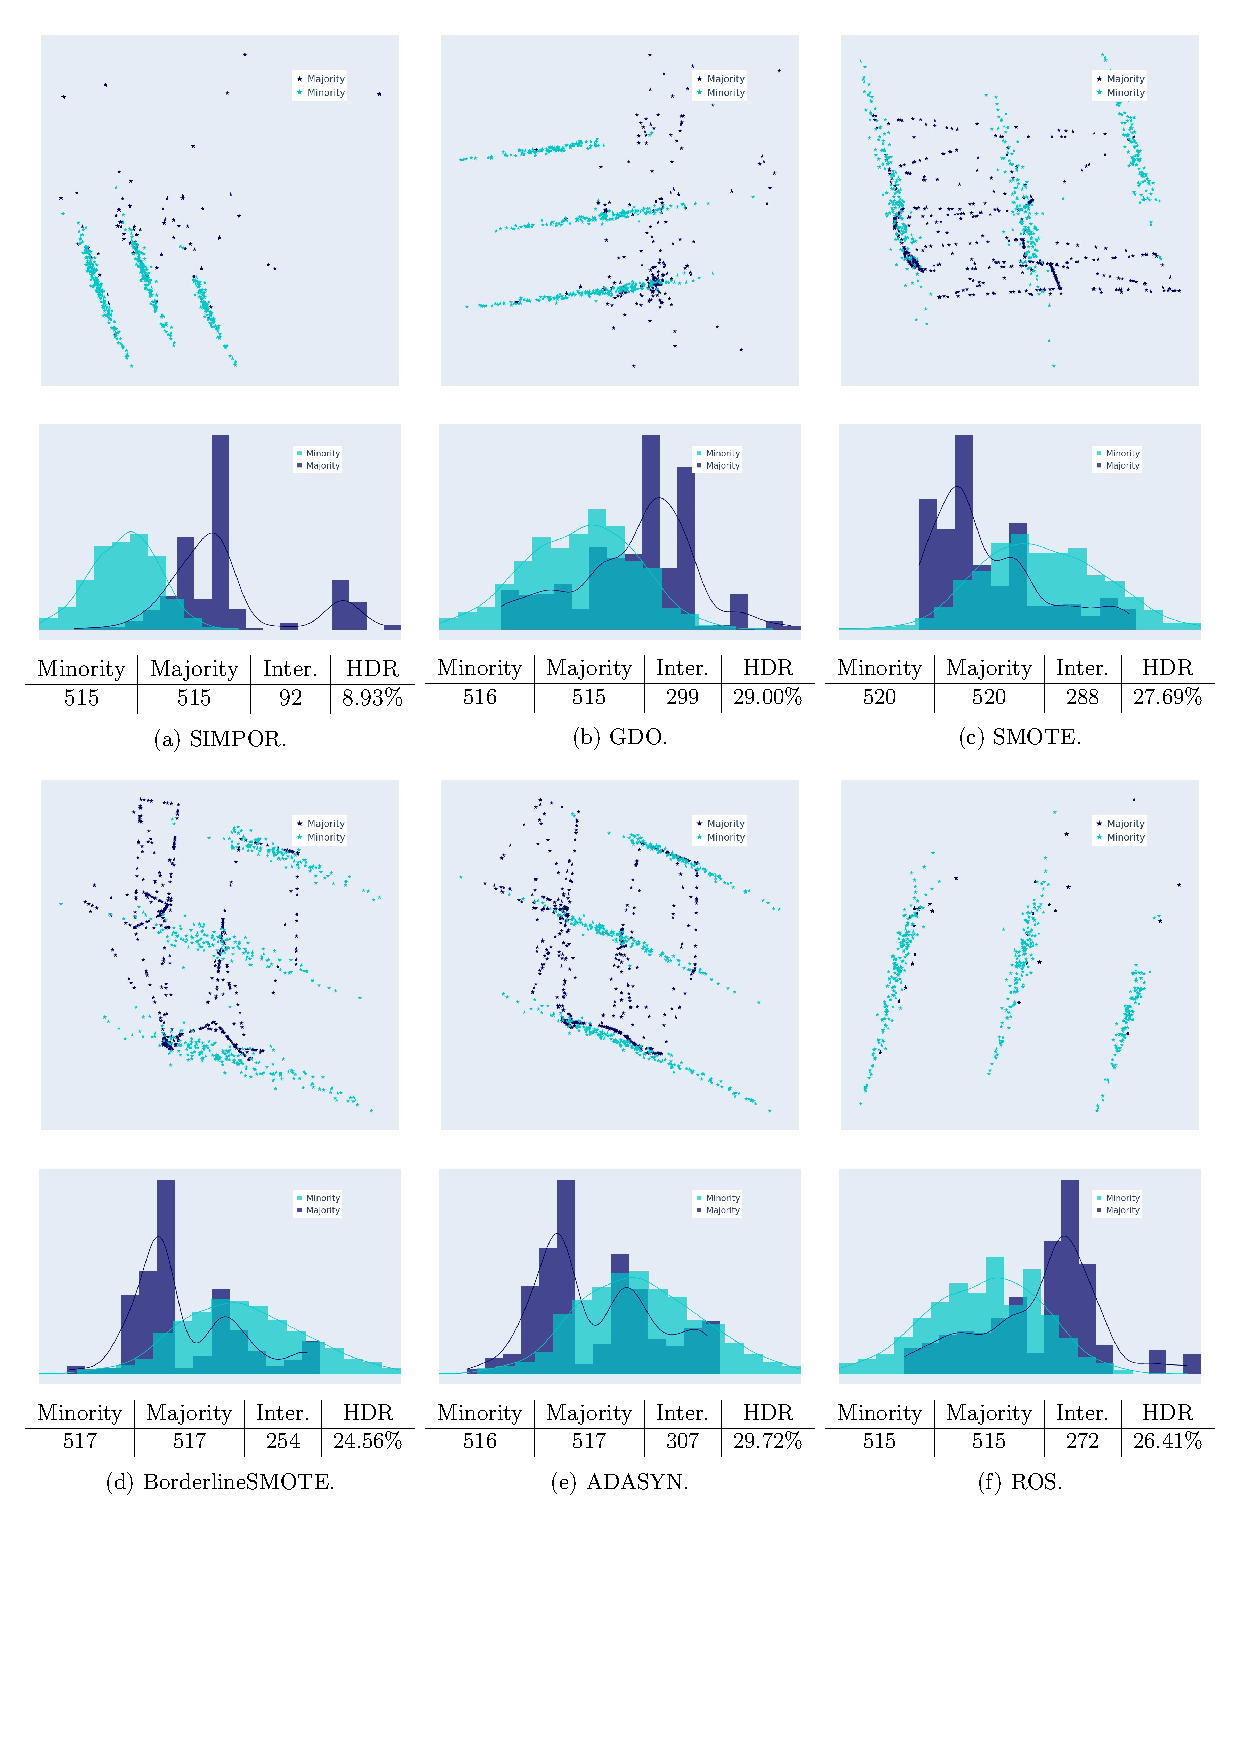
\includegraphics[width=0.8\linewidth,trim=10 90 10 10, clip ]{Figures/PCA/abalone9-18}
	\caption{Abalone9-18: Generated training data projected onto 2-dimension space and their histograms in 1-Dimension space using Principle Component Analysis dimension reduction technique. The bottom tables illustrate the number of samples in two classes, 1-Dimension histogram intersection between 2 classes, and the hard-to-differentiate ratio between the number of intersection samples to the number of minority samples ($HDR = \frac{Inter.}{Minority}100\%$).}
	\label{fig:visualization1d2d}
\end{figure*}

\R{histogramVisualization}
\Copy{histogramVisualization}{
To explore more on how the techniques perform, we visualize the generated data by projecting them onto lower dimension space (i.e., one and two dimensions) using the Principle Component Analysis technique (PCA) \cite{pca}. Data's 2-Dimension (2D) plots and 1-Dimension histograms are presented with a hard-to-differentiate ratio (HDR) for each technique. 1D histograms are computed by dividing one-dimensional-reduced data into 20 bins (intervals) and counting the number of samples within the interval of each bin. A hard-to-differentiate ratio is defined as the ratio of the number of samples in the intersection between 2 classes to the total of minority samples ($HDR = \frac{No.\: Intersection \: samples}{No. \: Minority \: samples}100\% $) where the number of intersection samples is estimated by counting samples in the overlapped bins between the two classes in the 1D histograms. This ratio is expected to be as small as 0\% if the two classes are well separated; in contrast, 100\% indicates that the two classes cannot be distinguished in the projected 1D space. Besides HDR, we show the absolute numbers of Minority, Majority, and Intersection samples for each technique in the bottom tables. From the plots, we observe how the data are distributed in 2D space and quantify samples that are hard to be differentiated in the 1D space histograms.       
}

To save space, we only show the plot of one dataset (i.e., Abalone9-18 dataset) in Figure \ref{fig:visualization1d2d}. Many other datasets are observed to have similar patterns. We observe that the proposed technique does not poorly generate synthetic samples as many as other techniques do. HDR results show that \Methodname{} achieves the least number of hard-to-differentiate ratio at 15.47\%. As shown in the 2D visualization sub-figures, other techniques poorly-place synthetic data crossed the other class. This causes by outliers or noises near the border between the two classes that other techniques do not pay attention to and mistakenly create more noise. In contrast, \Methodname{} safely produces synthetic data towards the minority class by maximizing the posterior ratio ;thus it can reduce the number of poorly-placed samples.
 
 
 
\Copy{processingTime}{ 
\begin{table}[htbp]
	\centering
	\caption{Processing time (in seconds) over 41 datasets.}
	\resizebox{0.97\columnwidth}{!}{%
		
	    \begin{tabular}{lcccccc}
	    	\toprule
	    	& SIMPOR & GDO   & SMOTE & BL-SMOTE & ADASYN & DeepSM \\
	    	\midrule
	    	glass1 & 0.1147 & 0.0576 & 0.0020 & 0.0033 & 0.0032 & 0.8587 \\
	    	wisconsin & 2.0805 & 0.1769 & 0.0024 & 0.0044 & 0.0046 & 1.2004 \\
	    	pima  & 0.2032 & 0.2066 & 0.0025 & 0.0049 & 0.0050 & 1.2297 \\
	    	glass0 & 0.2157 & 0.0553 & 0.0023 & 0.0035 & 0.0036 & 0.8601 \\
	    	yeast1 & 0.2457 & 0.4749 & 0.0035 & 0.0108 & 0.0104 & 1.4846 \\
	    	haberman & 0.0517 & 0.1560 & 0.0022 & 0.0033 & 0.0036 & 0.9246 \\
	    	vehicle1 & 0.4365 & 0.1237 & 0.0025 & 0.0059 & 0.0059 & 1.4147 \\
	    	vehicle2 & 6.2913 & 0.1512 & 0.0029 & 0.0053 & 0.0061 & 1.3976 \\
	    	vehicle3 & 0.2821 & 0.1237 & 0.0024 & 0.0060 & 0.0061 & 1.3487 \\
	    	creditcard & 2.1200 & 0.3783 & 0.0087 & 0.0184 & 0.0182 & 1.7980 \\
	    	glass-0-1-2-3\_vs\_4-5-6 & 0.3376 & 0.0459 & 0.0023 & 0.0035 & 0.0035 & 0.8407 \\
	    	vehicle0 & 7.3645 & 0.1198 & 0.0024 & 0.0054 & 0.0058 & 1.2953 \\
	    	ecoli1 & 0.0418 & 0.0337 & 0.0010 & 0.0018 & 0.0017 & 0.9310 \\
	    	new-thyroid1 & 0.5352 & 0.0304 & 0.0015 & 0.0024 & 0.0024 & 0.8590 \\
	    	new-thyroid2 & 0.3881 & 0.0359 & 0.0025 & 0.0033 & 0.0031 & 0.8747 \\
	    	ecoli2 & 0.2516 & 0.0266 & 0.0011 & 0.0017 & 0.0016 & 0.9733 \\
	    	glass6 & 0.3196 & 0.0268 & 0.0014 & 0.0025 & 0.0023 & 1.0744 \\
	    	yeast3 & 0.1374 & 0.2422 & 0.0023 & 0.0060 & 0.0059 & 1.6699 \\
	    	ecoli3 & 0.0658 & 0.0378 & 0.0015 & 0.0025 & 0.0024 & 0.9647 \\
	    	page-blocks0 & 7.9654 & 2.0918 & 0.0045 & 0.0143 & 0.0138 & 3.6029 \\
	    	yeast-2\_vs\_4 & 2.4310 & 0.0624 & 0.0017 & 0.0028 & 0.0028 & 1.0286 \\
	    	yeast-0-5-6-7-9\_vs\_4 & 0.0868 & 0.0632 & 0.0016 & 0.0029 & 0.0027 & 0.9809 \\
	    	vowel0 & 4.7675 & 0.1312 & 0.0018 & 0.0039 & 0.0037 & 1.2410 \\
	    	glass-0-1-6\_vs\_2 & 0.0482 & 0.0207 & 0.0013 & 0.0023 & 0.0022 & 0.9133 \\
	    	glass2 & 0.0501 & 0.0227 & 0.0013 & 0.0024 & 0.0024 & 0.8855 \\
	    	yeast-1\_vs\_7 & 0.4697 & 0.0420 & 0.0017 & 0.0026 & 0.0026 & 1.0355 \\
	    	glass4 & 0.1141 & 0.0197 & 0.0012 & 0.0024 & 0.0023 & 0.9469 \\
	    	ecoli4 & 0.1087 & 0.0310 & 0.0015 & 0.0024 & 0.0024 & 0.9393 \\
	    	page-blocks-1-3\_vs\_4 & 1.8742 & 0.0445 & 0.0015 & 0.0027 & 0.0026 & 0.9992 \\
	    	abalone9-18 & 2.9722 & 0.0716 & 0.0015 & 0.0028 & 0.0026 & 1.2095 \\
	    	yeast-1-4-5-8\_vs\_7 & 0.0881 & 0.0673 & 0.0017 & 0.0031 & 0.0028 & 1.0803 \\
	    	glass5 & 0.2815 & 0.0241 & 0.0017 & 0.0033 & 0.0036 & 0.8550 \\
	    	yeast-2\_vs\_8 & 0.1239 & 0.0441 & 0.0016 & 0.0027 & 0.0028 & 0.9849 \\
	    	car\_eval\_4 & 0.4381 & 0.1746 & 0.0026 & 0.0066 & 0.0049 & 1.6616 \\
	    	wine\_quality & 0.1622 & 0.8587 & 0.0030 & 0.0144 & 0.0137 & 3.3128 \\
	    	yeast\_me2 & 0.1060 & 0.1379 & 0.0018 & 0.0042 & 0.0039 & 1.7350 \\
	    	yeast4 & 0.1083 & 0.1386 & 0.0018 & 0.0041 & 0.0039 & 1.6314 \\
	    	yeast-1-2-8-9\_vs\_7 & 0.0924 & 0.0757 & 0.0017 & 0.0031 & 0.0030 & 1.3069 \\
	    	yeast5 & 0.1188 & 0.1312 & 0.0019 & 0.0037 & 0.0040 & 1.6181 \\
	    	yeast6 & 0.0613 & 0.1419 & 0.0018 & 0.0037 & 0.0036 & 1.6382 \\
	    	abalone19 & 0.0890 & 0.3161 & 0.0022 & 0.0053 & 0.0054 & 3.0168 \\
	    	\bottomrule
	    \end{tabular}%
		
	}
	\label{tab:ProcessingTime}%
\end{table}%

\subsection{Processing Time.}
\label{sec:processingTime}
Data processing times for oversampling-based approaches on 41 datasets are compared to provide a more comprehensive comparison. We don't compare them to the other approaches, i.e., cost-sensitive learning and ensemble learning, because they only need negligible data processing time as they focus on classifiers other than improving the data. The processing time was recorded from our machine, which uses an Intel i7 32-thread processor and two NVIDIA 3090 Ti GPUs. 
Table \ref{tab:ProcessingTime} shows the recorded processing time over 41 datasets. Overall, our technique takes longer than others as we have to compute the kernel estimation for each data point, as mentioned in Section \ref{sec:implementation}. Similarly, DeepSMOTE generally suffers high time consuming cost because it heavily relies on underlying heuristic methods. In other words, the proposed technique is slower, but it provides better F1 and AUC scores than others.

}

\begin{figure*}[ht]
	\centering
	%[trim=left bottom right top, clip]
	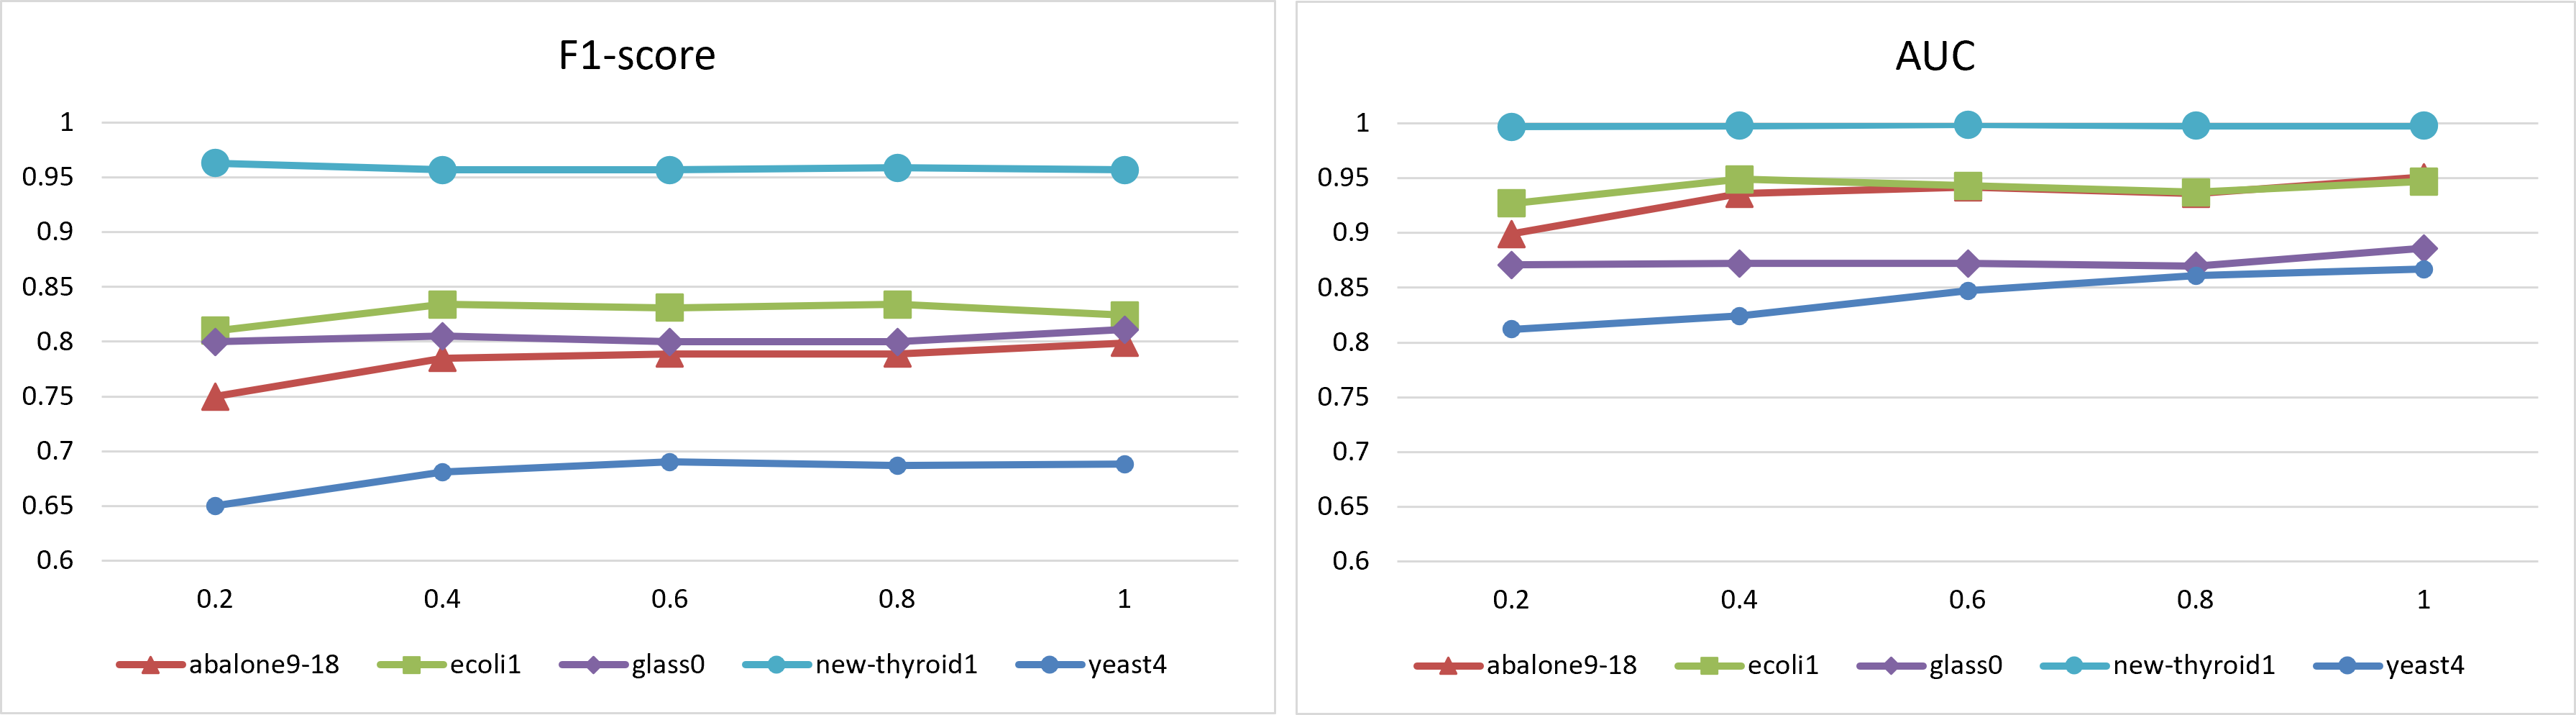
\includegraphics[width=0.98\linewidth, trim=5 10 10 10, clip ]{Figures/r_impact}
	\caption{F1-score and AUC results with varying Gaussian standard deviation (ranging from 0.2R to R).}
	\label{fig:r_result}
\end{figure*}

\begin{figure*}[h]
	\centering
	%[trim=left bottom right top, clip]
	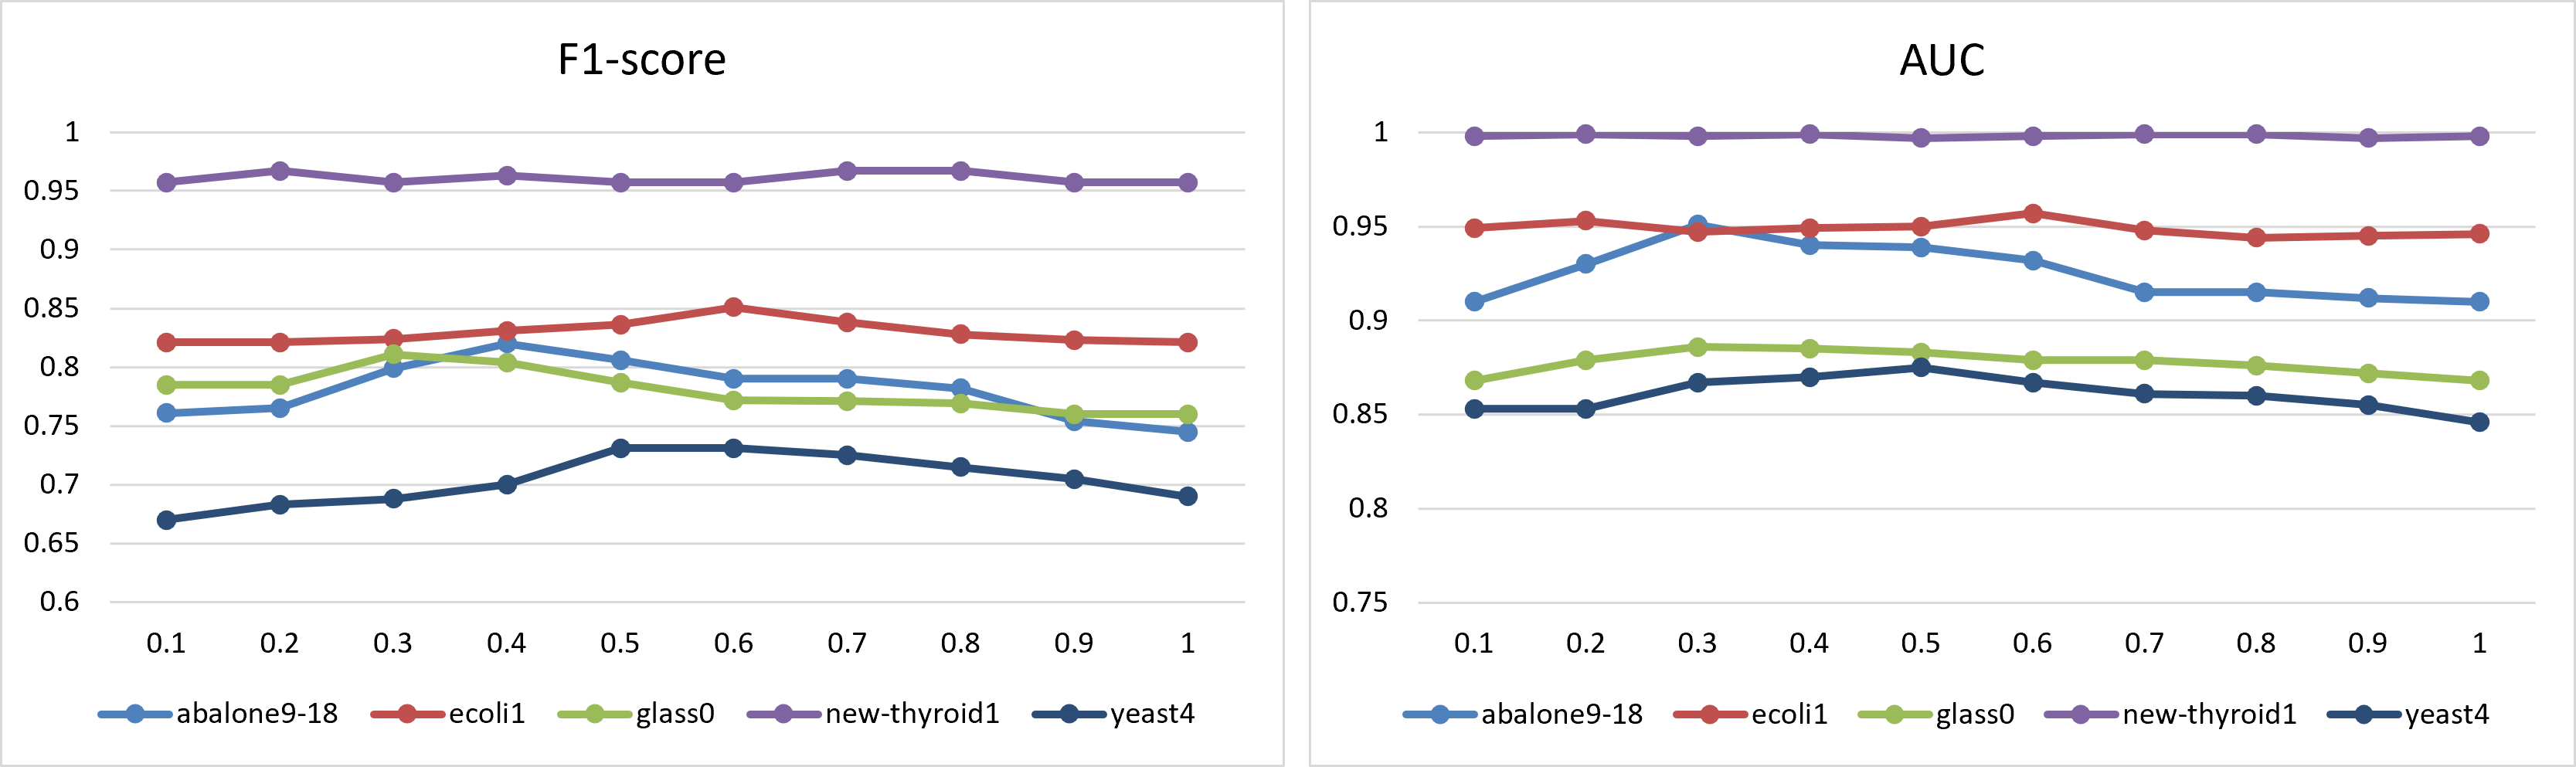
\includegraphics[width=0.98\linewidth, trim=5 10 10 10, clip ]{Figures/threshold_impact}
	\caption{F1-score and AUC results with varying informative portion IP.}
	\label{fig:ip_result}
\end{figure*}

\subsection{Empirical study on the impact of radius factor r.}
\label{sec:simpor_r_distribution_impact}
In this section, we study how the classification performance is impacted by different generation radius factor $r$ in Equation \ref{equ:r_dist}. The classification performance is measured under different distribution settings of the radius r as it controls how far synthetic data are generated from its original minority sample. We use different parameters for the Gaussian distribution $\mathcal{N}(\mu ,\,{(\alpha R)}^{2})$. Particularly, we fix the mean value to zero and change $\alpha$ from 0.2 to 1 with steps of 0.2 so that the Gaussian standard deviation $\alpha R$ will range from 0.2R to R. To save space, we arbitrarily select 5 datasets to conduct this experiment. The classification results are shown in Figure \ref{fig:r_result}. 

\R{EmpiricalExplanation}
\Copy{EmpiricalExplanation}{
The figure obtained from the experiment indicates that the r factor, with a radius distribution standard deviation ranging from 0.6R to R, has minimal impact on the classification performance. While there are slight variations within the $\alpha$ range of 0.6 to 1, the performance improves between 0.2 to 0.6 (such as for ecoli1, abalone9-18, and yeast4). This is because the performance mainly depends on the classifier's decision boundary, and the synthetic data are placed far away from the decision boundary towards the minority class area; thus,  the radius does not have much effect on the accuracy results. However, in the case of multi-classed data, the performance might be affected by a significant value of R. 
}
\subsection{Empirical study on the impact of informative portion (IP).}
This section studies the empirical impact of the informative portion (IP) in Section \ref{sec:EAL}. This portion works as a threshold to adjust how many samples are taken into consideration of informative samples. To save space, we study five datasets used in Section \ref{sec:simpor_r_distribution_impact}. Different values of IP ranging from 0.1 to 1 are applied, and the classification performance results are shown in Figure \ref{fig:ip_result}.

\R{EmpiricalExplanationIP}
\Copy{EmpiricalExplanationIP}{
As we can see from the figure, while datasets with outstanding performance (new-thyroid1, ecoli1) have little impact, there are fluctuations in other datasets' F1-score and AUC score  (abalonce9-18, glass0, yeast4). This is because, for the easy-separated dataset such as new-thyroid1 and ecoli1, the IP change does not affect the classification performance as the data classes are easily separated. While in more challenging datasets, IP changes might affect the balance at the informative region; thus, this leads to performance variations. The resulting figure also suggests tuning IP for each dataset between a range of (0.2, 0.6) could achieve higher performance.
}










\section {Conclusion}
\label{sec:conclusion}
We propose a data balancing technique by generating synthetic data for minority samples maximizing the posterior ratio to embrace the chance they fall into the minority class and do not fall across the expected decision boundary. While maximizing the posterior ratio, we use kernel density estimation to estimate the likelihood so that it is able to work with complex distribution data without requiring data distribution assumptions. In addition, our technique leverage entropy-based active learning to find and balance the most informative samples. This is important to improve model performance as shown in our experiments on 41 real-world datasets. For future work, we would like to investigate the class imbalance for image data type and enhance our technique to adapt to image datasets.     




\newcommand{\argmin}[1]{\underset{#1}{\operatorname{arg}\,\operatorname{min}}\;}
\newcommand{\minmax}[1]{\underset{#1}{\operatorname{min}\,\operatorname{max}}\;}	
\newcommand{\prob}[1]{p_#1} 	

\newtheorem{example}{\bf Example}
\newtheorem{definition}{\bf Definition}
\newtheorem{theorem}{\bf Theorem}
\newtheorem{claim}{\bf Claim}
\newtheorem{proposition}{\bf Proposition}
\newtheorem{lemma}{\bf Lemma}
\newtheorem{remark}{\bf Remark}
\newtheorem{collolary}{\bf Collolary}


\newcommand{\Name}{AutoGAN-based Dimension Reduction for Privacy Preservation}
\newcommand{\shortName}{AGDRPP}

\newcommand{\ChapterPathAutoGAN}{Chapter4}

\chapter[AutoGAN-Based Dimension Reduction for Privacy Preservation]{AutoGAN-Based Dimension Reduction for Privacy Preservation \footnotemark }
\footnotetext{This chapter was published in Journal of Neurocomputing.
Permission is included in Appendix A.}

\label{chap:AUTOGAN}


\section{Introduction}
\label{sec:introduction}


Machine Learning (ML) is an important aspect of modern applications that rely on big data analytics (e.g., an on-line system collecting data from multiple data owners). However, these applications are progressively raising many different privacy issues as they collect different types of data on a daily basis. For example, many types of data are being collected in smart cities such as patient records, salary information, biological characteristics, Internet access history, personal images and so on. These types of data then can be widely used in daily recommendation systems, business data analysis, or disease prediction systems which in turn affect the privacy of individuals who contributed their sensitive data. Considering a multi-level access control system of a company using biometric recognition (e.g., face recognition, fingerprint) for granting permission to access data resources, the company staff members may concern their biological information being vulnerable to adversaries. Even though the utility of these biometric features can be effectively used in machine learning tasks for authentication purpose, leaking this information might lead to privacy breaches. For example, an adversary could utilize them to determine the members' identities.

Several tools and methods have been developed to preserve the privacy in machine learning applications, such as homomorphic encryption \cite{Bost2015,Emekci2007,Hesamifard2017}, secure multi-party computing \cite{Yao1986,Shamir1979}, differential privacy (DP) \cite{Chaudhuri,Zhang2012,Phan2016,Abadi2016,XiaoqianJiangZhanglongJiShuangWangNomanMohammedSamuelCheng2013}, compressive privacy \cite{zhuang2017fripal,GAP,DBLP:journals/corr/abs-1809-08911,DifferentialPrivacywithCompression,7815484, Kung, XieKun} and so on. Typically, differential privacy-based methods aim at preventing leaking individual information caused by queries. However, they are not designed to serve large number of queries since they require adding huge amount of noise to preserve privacy, thus significantly decreasing the ability to learn meaningful information from data. On the other hand, homomorphic encryption-based methods can be used to privately evaluate a function over encrypted data by a third party without accessing to plain-text data, hence the privacy of data owners can be protected. However, due to the high computational cost and time consumption, they may not work with a very large dataset, normally required in ML applications.

In this study, we consider an access control system collecting dimension-reduced face images of staff members to perform authentication task and to provide permission for members who would like to access company's data resources (Figure \ref{fig:attackmodel}). We propose a non-linear dimension reduction framework to decrease data dimension for the authentication purpose mentioned above and to protect against an adversary from reconstructing member images. Firstly, we introduce $\epsilon$-DR Privacy as a theoretical tool for dimension reduction privacy evaluation. It evaluates the reconstruction distance between original data and reconstructed data of a dimension reduction (DR) mechanism. This approach encourages a DR mechanism to enlarge the distance as high distance yields high level of privacy. While other methods such as differential privacy-based methods rely on inference uncertainty to protect sensitive data, $\epsilon$-DR Privacy is built on reconstruction error to evaluate privacy. Therefore, unlike differential privacy methods,  $\epsilon$-DR Privacy is not negatively impacted by the number of queries. Secondly, as detailed in Section \ref{sec:autogan_methodology}, we recommend a privacy-preserving framework Autoencoder Generative Adversarial Nets-based Dimension Reduction Privacy (AutoGAN-DRP) for enhancing data owner privacy and preserving data utility. The \textit{utility} herein is evaluated via machine learning task performance (e.g., classification accuracy).

Our dimension reduction (DR) framework can be applied to different types of data and used in several practical applications without heavy computation of encryption and impact of query number. The proposed framework can be applied directly to the access control system mentioned above. More elaboratively, face images are locally collected, nonlinearly compressed to achieve DR, and sent to the authentication center. The server then performs classification tasks on the dimension-reduced data. We assume the authentication server is semi-honest, that is to say it does not deviate from authenticating protocols while being curious about a specific member's identity. Our DR framework is designed to resist against reconstruction attacks from a strong adversary who obtains the training dataset and the transformation model. 

During the stage of experiments, we implemented our framework to evaluate dimension-reduced data in terms of accuracy of the classification tasks, and we attempted to reconstruct original images to examine the capacity of adversaries. We performed several experiments on three facial image datasets in both gray-scale and color, i.e., \textit{the Extended Yale Face Database B} \cite{GeBeKr01}, \textit{AT}\&\textit{T} \cite{341300}, and \textit{CelebFaces Attributes Dataset (CelebA)} \cite{celeba}. The experiment results illustrate that with only seven reduced dimensions our method can achieve accuracies of 93\%, 90\%, and 80\% for AT\&T, YaleB, and CelebA respectively. Further, our experiments show that at the accuracies of 79\%, 80\% and 73\% respectively, the reconstructed images could not be recognized by human eyes. In addition, the comparisons shown in Section \ref{sec:AutoGAN_DP_PCA} also illustrate that AutoGAN-DRP is more resilient to reconstruction attacks compared to related works.
Our work has two main contributions:
\begin{enumerate}
\item To analytically support privacy guarantee, we introduce $\epsilon$-DR Privacy as a theoretical approach to evaluate privacy preserving mechanism.
\item We propose a non-linear dimension reduction framework for privacy preservation motivated by Generative Adversarial Nets \cite{Goodfellow2014} and Auto-encoder Nets \cite{Baldi2012}. 
  
\end{enumerate}
The rest of this chapter is organized as follows. Section \ref{sec:autogan_relatedwork} summarizes state-of-the-art privacy preservation machine learning (PPML) techniques and reviews knowledge of deep learning methods including generative adversarial neural nets and Auto-encoder. Section \ref{sec:autogan_methodology} describes the privacy problem through a scenario of a facial recognition access control system, introduces the definition of $\epsilon$-DR Privacy to evaluate DR-based privacy preserving mechanisms, and presents our framework \Name. Section \ref{sec:experimentsanddiscussion} presents and discusses our experiment results over three different face image datasets. Section \ref{sec:AutoGAN_GAP} compares AutoGAN-DRP to a similar work GAP in terms of reconstruction error and classification accuracy. Section \ref{sec:AutoGAN_DP_PCA} demonstrates reconstructed images over AutoGAN-DRP and other privacy preservation techniques (i.e., Differential Privacy and Principle Component Analysis). Finally, the conclusion and future work are mentioned in Section \ref{sec:Autogan_conclusion}. 

	
\section{Related Work}
\label{sec:autogan_relatedwork}
\subsection{Literature Review}

Machine learning privacy preservation methods are categorized into two main approaches. Cryptographic approach applies to the scenarios where the data owners do not wish to expose their plain-text sensitive data while asking for machine learning services from a third-party. The most common tool used in this approach is fully homomorphic encryption that supports multiplication and addition operations over encrypted data, which enabling the ability to perform a more complex function. However, the high cost of the multiplicative homomorphic operations renders it difficult to be applied on machine learning tasks. In order to avoid multiplicative homomorphic operations, additive homomorphic encryption schemes are more widely used in privacy preserving machine learning (PPML). However, the limitation of the computational capacity in additive homomorphic schemes narrows the ability to apply on particular ML techniques. Thus, such additive homomorphic encryption-based methods in \cite{Bost2015,Emekci2007,Raphael,Hesamifard}  are only applicable to simple machine learning algorithms such as decision tree and naive bayes. In Hesamifard's work \cite{Hesamifard2017},the fully homomorphic encryption is applied to perform deep neural networks over encrypted data, where the non-linear activation functions are approximated by polynomials. 
  
In secure multi-party computing (SMC), multiple parties collaborate to compute functions without revealing plain-text to other parties. A widely-used tool in SMC is garbled circuit \cite{Yao1986}, a cryptographic protocol carefully designed for two-party computation, in which they can jointly evaluate a function over their sensitive data without the trust of each other. In \cite{Al-rubaie}, Mohammad introduced a SMC protocol for principle component analysis (PCA) which is a hybrid system utilizing additive homomorphic and garbled circuit. In secret sharing techniques \cite{Shamir1979}, a secret \textbf{s} is distributed over multiple pieces \textbf{n} also called \textit{shares}, where the secret can only be recovered by a sufficient amount of \textbf{t} \textit{shares}. A good review of secret sharing-based techniques and encryption-based techniques for PPML is given in \cite{Pedersen2007}. Although these encryption-based techniques can protect the privacy in particular scenarios, their computational cost is a significant concern. Furthermore, as \cite{Pedersen2007} elaborated, the high communication cost also poses a big concern for both techniques.
      
The other category is Non-Cryptographic approach. For example, Differential Privacy (DP) \cite{Dwork2006} aims to prevent membership inference attacks. DP considers a scenario that an adversary infers a member's information based on the difference of outputs of a ML mechanism before and after the member join a database. The database with the member's information and without the member's information can be considered as two neighbor databases which differ by at most one element. DP adds noise to the outputs of the ML mechanism to result in similar outputs from the two neighbor databases. Thus, adversaries cannot differentiate the difference between the two databases. A mechanism M satisfies $\epsilon$-differential privacy if for any two neighbor databases $D$ and $D'$, and any subset S of the output space of M satisfies 
$ Pr[M(D) \in S] \leq e^{\epsilon}  Pr[M(D') \in S]  $. 
The similarity of query outputs protects a member information from such membership inference attacks. The \textit{similarity} is guaranteed by the parameter $\epsilon$ in a mechanism in which the smaller $\epsilon$ provides a better level of privacy preservation. \cite{Chaudhuri, Zhang2012,NIPS2008, Wu, MYang} propose methods to guarantee $\epsilon$-differential privacy by adding noise to outcome of the weights $w^*= w + \eta$, where $\eta$ drawn from Laplacian distribution and adding noise to the objective function of logistic regression or linear regression models. \cite{Phan2016,Abadi2016} satisfy differential privacy by adding noise to the objective function while training a deep neural network using stochastic gradient descent as the optimization algorithm. 

In addition, there are existing works proposing differential privacy dimension reduction. One can guarantee $\epsilon$-differential privacy by perturbing dimension reduction outcome. Principal component analysis (PCA) whose output is a set of eigenvectors is a popular method in dimension reduction. The original data is then represented by its projection on those eigenvectors, which keeps the largest variance of the data. One can reduce the data dimension by eliminating insignificant eigenvectors which contain less variance, and apply noise on the outcome to achieve differential privacy\cite{XiaoqianJiangZhanglongJiShuangWangNomanMohammedSamuelCheng2013}. However, the downside of these methods is that they are designed for specific mechanisms and datasets and not working well with the others. For example, record-level differential privacy is not effectively used with image dataset as shown in \cite{Hitaj2017}. Also, the amount of added noise is accumulative based on the number of queries so that this approach usually leads to low accuracy results with a high number of queries. 

Similar to our work, Generative Adversarial Privacy (GAP) \cite{GAP} is a perturbation method utilizing the minimax algorithm of Generative Adversarial Nets to preserve privacy and to keep utility of image datasets. GAP perturbs data within a specific $l_2$ distance constraint between original and perturbed data to distort private class labels and at the same time preserve non-private class labels. However, it does not protect the images themselves, and an adversary can visually infer private label (e.g., identity) from images. In contrast, our method protects an image by compressing it into a few dimension vector and then transferring without clearly exposing the original image.

 



	
\subsection{Preliminaries}
	To enhance the distance between original and reconstructed data in our DR system, we utilize the structure of Generative Adversarial Network (GAN) \cite{Goodfellow2014} for data perturbation and deep Auto-encoder \cite{Baldi2012} for data reconstruction. The following sections briefly review Auto-encoder and GAN.
\subsubsection{Auto-encoder}
Auto-encoder is aimed at learning lower dimension representations of unsupervised data. Auto-encoder can be used for denoising and reducing data dimension. It can be implemented by two neural network components: \textit{encoder} and \textit{decoder}. The \textit{encoder} and \textit{decoder} perform reverse operations. The input of the \textit{encoder} is the original data while the output of the \textit{decoder} is expected to be similar to the input data. The middle layer extracts latent representation of original data that could be used for dimension reduction. An Auto-encoder training process can be described as a minimization problem of the auto-encoder's loss function $\mathcal{L(\cdot)}$:
\begin{equation}
\mathcal{L}(x,g(f(x)))
\end{equation}
where x is input data, f($\cdot$) is an encoding function, and g($\cdot$) is a decoding function.

\subsubsection{GAN}
Generative Adversarial Nets is aimed at approximating distribution $p_d$ of a dataset via a generative model. GAN simultaneously trains two components \textit{generator} $G$ and \textit{discriminator} $D$, and the input of $G$ is sampled from a prior distribution $p_z(z)$ through which $G$ generates fake samples similar to the real samples. At the same time, $D$ is trained to differentiate between fake samples and real samples, and send feedback to $G$ for improvement. GAN can be formed as a two-player minimax game with value function V(G,D):

\begin{equation}
	\begin{split}
		\min_G \max_D{V(G,D)} = & E_{x \sim \prob{d}} [log(D(x))] + \\& E_{z\sim \prob{z} }[log( 1 - D( G(z) ))]
	\end{split}
\end{equation}

The two components, \textit{Generator} and \textit{Discriminator} can be built from neural networks (e.g., fully connected neural network, convolutional neural network). The goal of G is to reduce the accuracy of D. Meanwhile, the goal of D is to differentiate fake samples from real samples. These two components are trained until the discriminator cannot distinguish between generated samples and real samples.


\section{Methodology} \label{sec:autogan_methodology}

In this section, we first describe the problem and threat model, then we introduce a definition of DR-Privacy and our dimensionality reduction method (AutoGAN-DRP).    

  
\begin{figure}[h]
	\includegraphics[width=\linewidth]{\ChapterPathAutoGAN/figures/AttackModel_CP}
	\caption{Attack model.}
	\label{fig:attackmodel}
\end{figure} 

\subsection{Problem Statement}
We introduce the problem through the practical scenario mentioned in Section \ref{sec:introduction}. Figure \ref{fig:attackmodel} briefly describes the entire system in which staff members (clients) in a company request access to company resources, such as websites and data servers through a face recognition access control system. For example, if member n requests to access web server 2, the local device first takes a facial photo of the member by an attached camera, locally transforms it into lower dimension data, and sends to an authentication center. The authentication server then obtains the low dimensional data and determines member access eligibility by using a classifier without clear face images of the requesting member. We consider that the system has three levels of privileges (i.e., single level, four-level, eight-level) corresponding to three groups of members. We assume the authentication server is semi-honest (it obeys work procedure but might be used to infer personal information). If the server is compromised, an adversary in the authentication center can reconstruct the face features to achieve plain-text face images and determine members' identity.  
\subsection{Threat Model}
In the above scenario, we consider that a strong adversary who has access to the model and training dataset attempts to reconstruct the original face images for inferring a specific member's identity. Our attack model can be represented in Figure \ref{fig:attackmodel}. The adversary utilizes training data and facial features to identify a member identity by reconstructing the original face images using a reconstructor in an auto-encoder. Rather than using fully connected neural network, we implement the auto-encoder by convolutional neural network which more effective for image datasets. Our goal is to design a data dimension reduction method for reducing data dimension and resisting full reconstruction of original data.  



\subsection{$\epsilon$-Dimension Reduction Privacy ($\epsilon$-DR Privacy)} \label{sec:theory}


\begin{figure}[H]
	\centering
	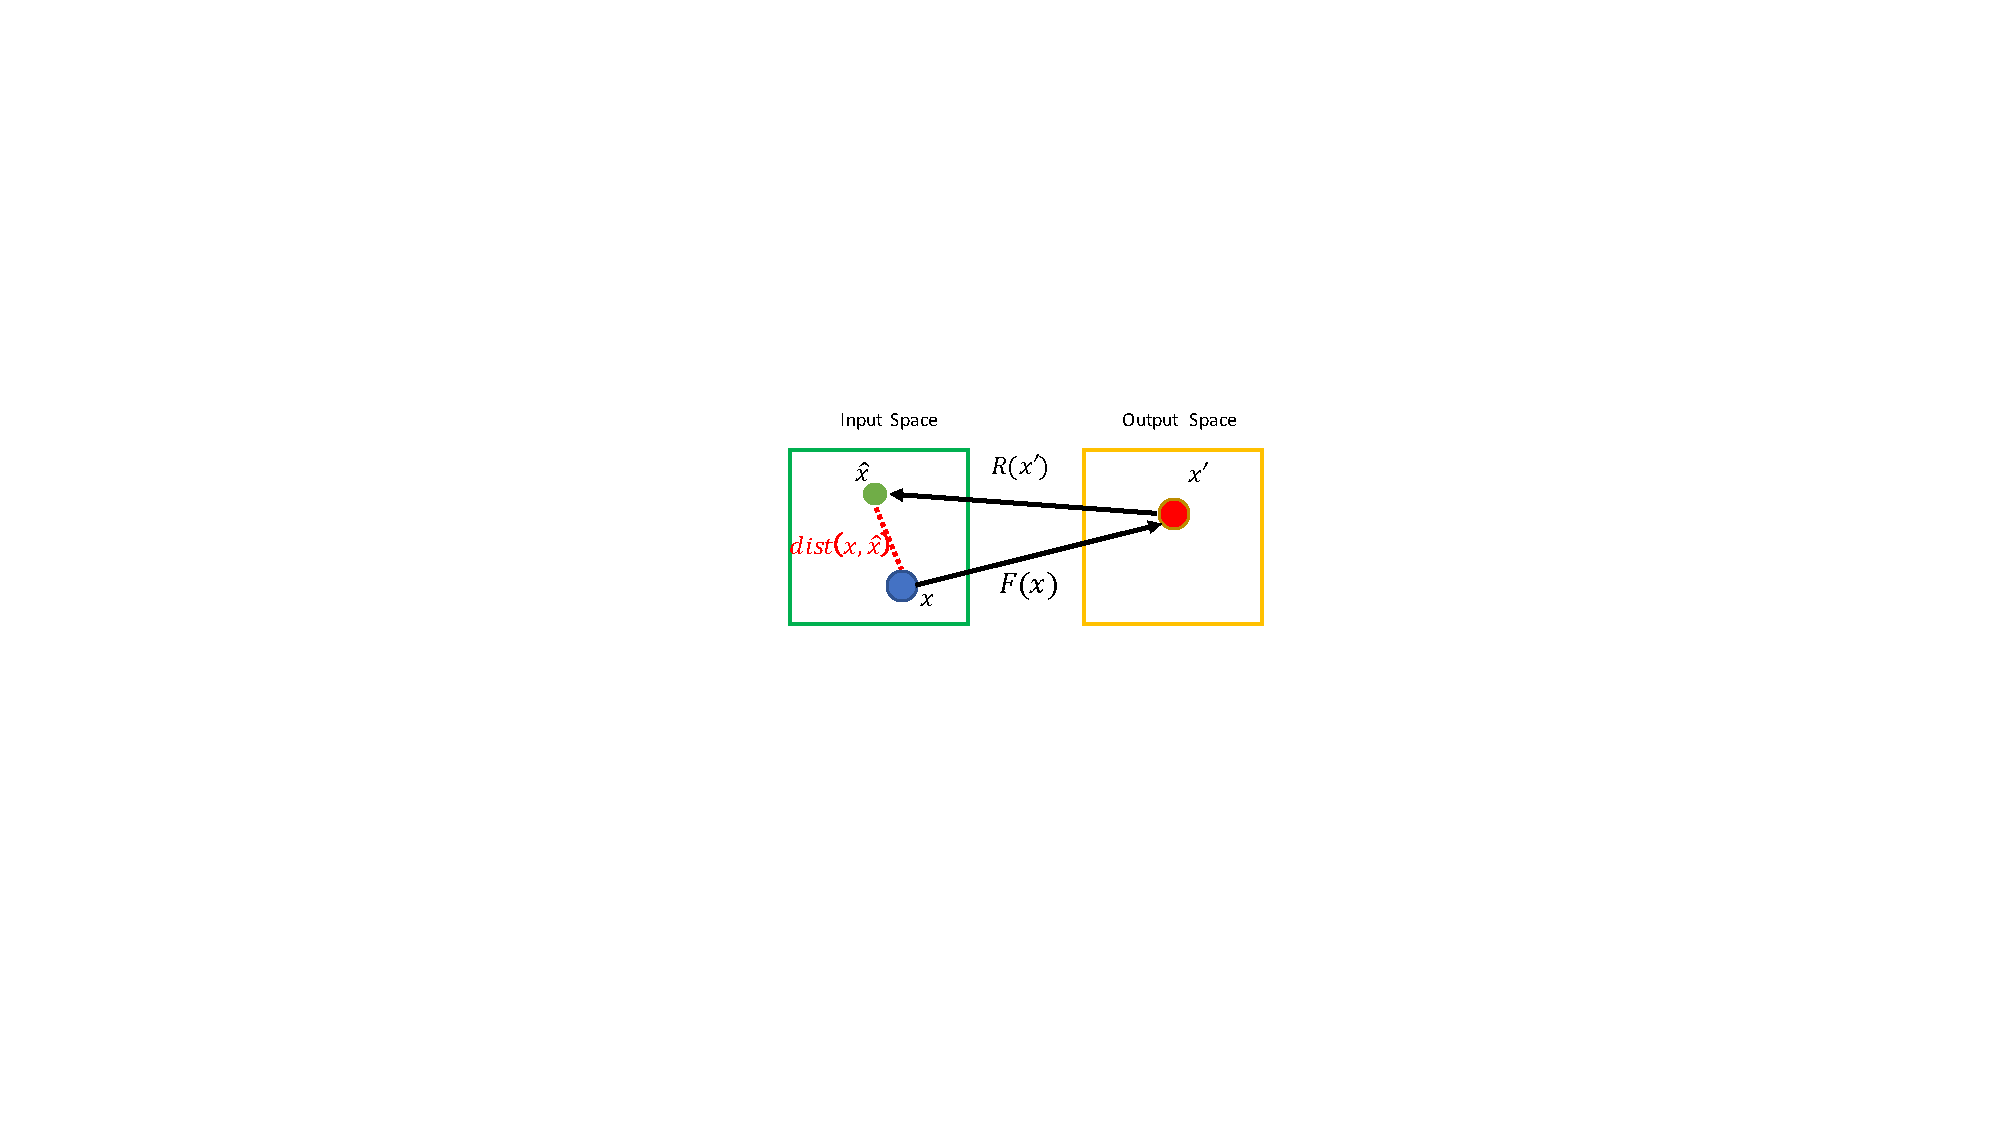
\includegraphics[width=0.4\textwidth]{\ChapterPathAutoGAN/figures/DR_P_CP}
	\caption{DR projection and reconstruction.} 
	\label{fig:DRP}
\end{figure} 

%\section{$\epsilon$-Dimension Reduction Privacy ($\epsilon$-DR Privacy)}
We introduce the Dimension Reduction Privacy (DR-Privacy), and define a formal definition of the $\epsilon$-DR Privacy to mathematically quantify/evaluate the mechanisms designed to preserve the DR-Privacy 
% the privacy that has been preserved
via dimension reduction. The DR-Privacy aims to achieve privacy-preserving via dimension reduction, which refers to transforming the data into a lower dimensional subspace, such that the private information is concealed while the underlying probabilistic characteristics are preserved, which can be utilized for machine learning purposes. To quantify the DR-Privacy and guide us to design such DR functions, we define $\epsilon$-DR Privacy as follows.


{\bf Definition 1}: ($\epsilon$-DR Privacy) A Dimension Reduction Function $F(\cdot)$ satisfies $\epsilon$-DR Privacy if for each i.i.d. $m$-dimension input sample $x$ drawn from the same distribution $D$, and for a certain distance measure $dist(\cdot)$, we have
\begin{equation}
\begin{split} \label{eq:modularity}
\mathbb{E}[dist(x, \hat{x})] \geq \epsilon
\end{split}
\end{equation}
where $\mathbb{E}[\cdot]$ is the expectation, $\epsilon \geq 0$, $x^{\prime}=F(x)$, $\hat{x}=R(x^{\prime})$, and $R(\cdot)$ is the Reconstruction Function.

For instance, as shown in Fig.~\ref{fig:DRP}, given original data $x$, our framework utilizes certain dimension reduction function $F(x)$ to transform the original data $x$ into the transformed data $x^{\prime}$. The adversaries aim to design a corresponding reconstruction function $R(x^{\prime})$ such that the reconstructed data $\hat{x}$ would be closed/similar to the original data $x$. DR-Privacy aims to design/develop such dimension reduction functions, that the distance between the original data and its reconstructed data would be large enough to protect the privacy of the data owner.





\begin{figure}
	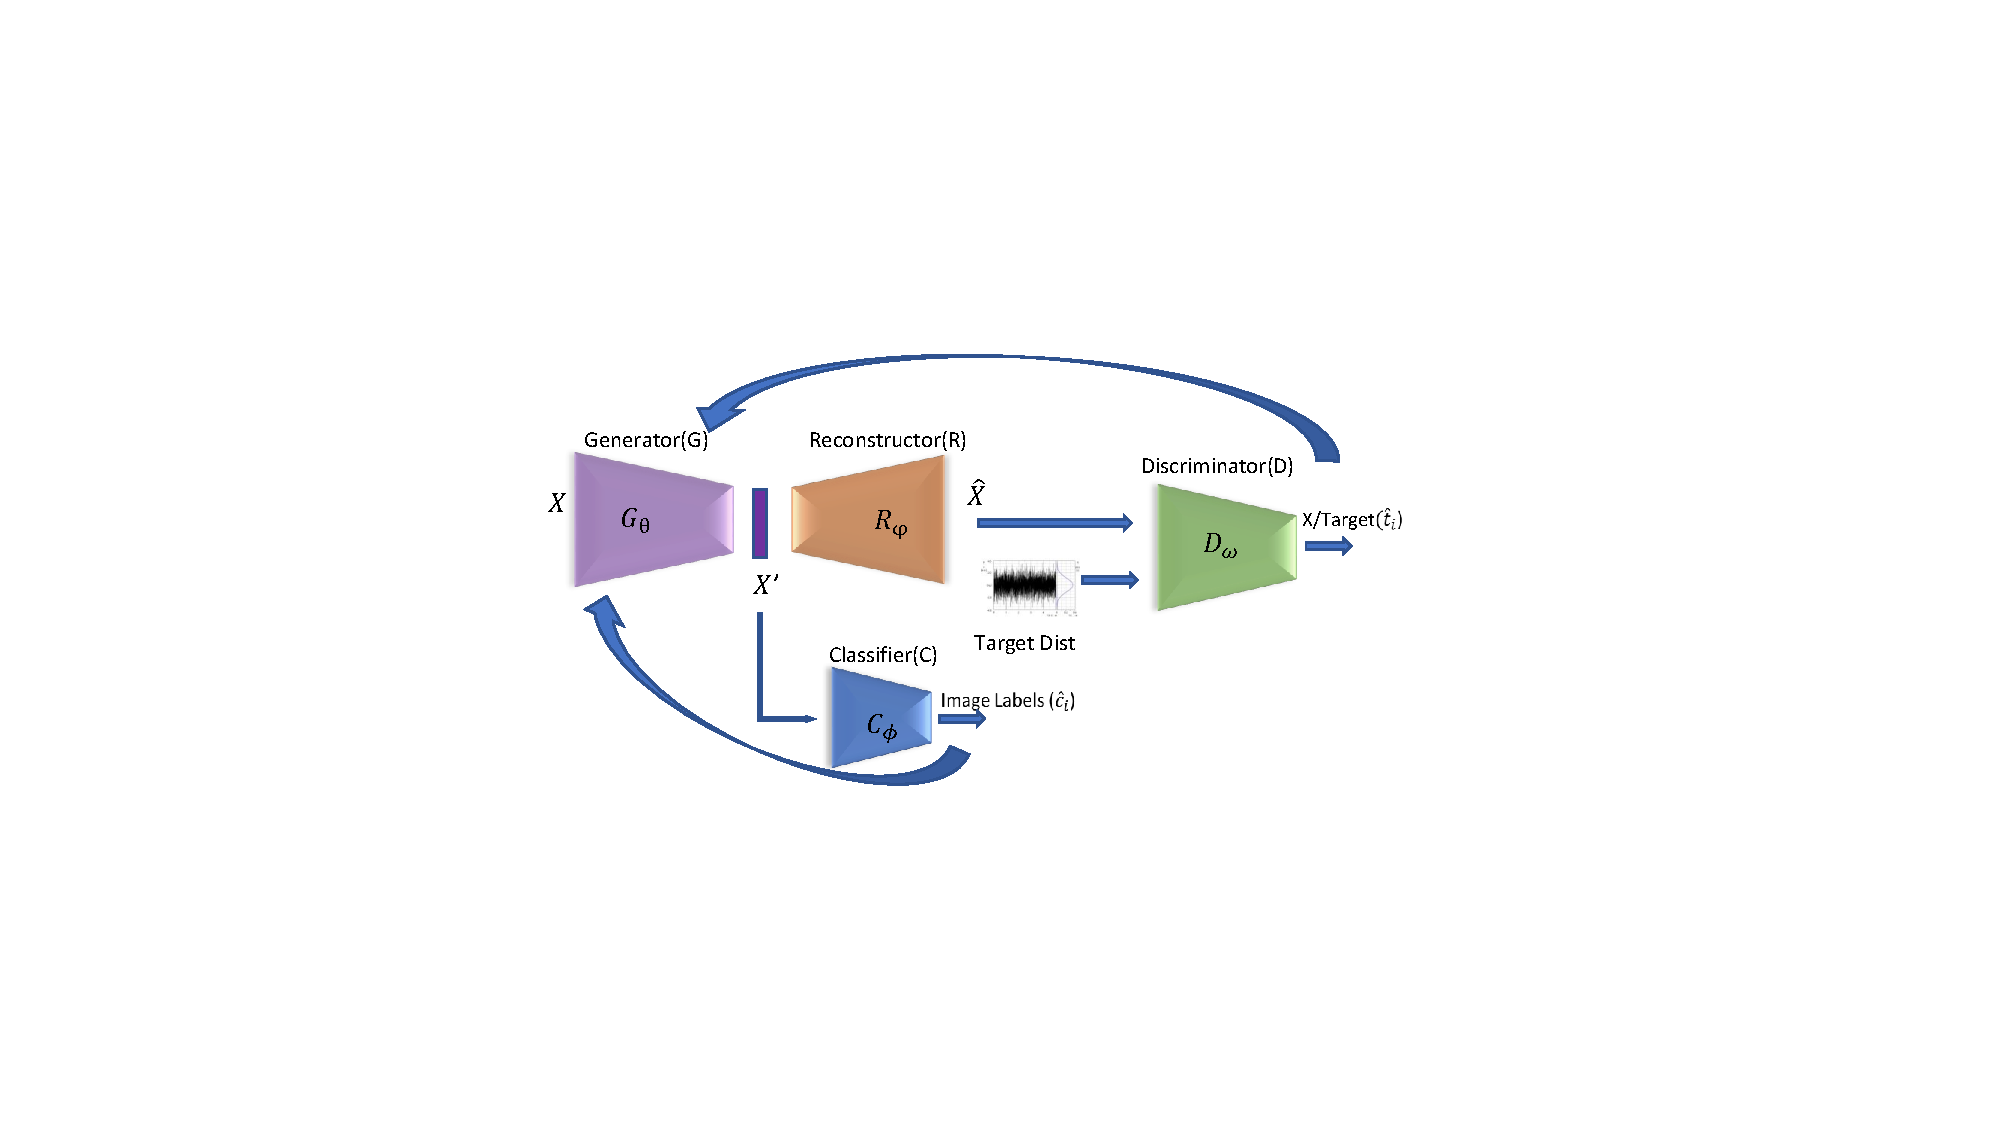
\includegraphics[width=\linewidth, trim= 8.5cm 5.5cm 8.5cm 5.5cm, clip=true]{\ChapterPathAutoGAN/figures/eGAN}
	\caption{AutoGAN-DRP}
	\label{fig:eGAN}
\end{figure}


\subsection{AutoGAN Dimension Reduction for Privacy Preserving}

We propose a deep learning framework for transforming face images to low dimensional data which is hard to be fully reconstructed. The framework can be presented in Figure \ref{fig:eGAN}. We leverage the structure of an auto-encoder \cite{Baldi2012} which contains encoder and decoder (in this work, we called them generator and re-constructor) in order to reduce data dimension. More specifically, the low dimensional representations are extracted from the middle layer of the auto-encoder (the output of the generator). The dimension-reduced data can be sent to the authentication server as an authentication request. We consider an adversary as a re-constructor implemented by a decoder. To resist against fully reconstructing images, the framework utilizes a discriminator in GAN \cite{Goodfellow2014} to direct reconstructed data to a designated target distribution with an assumption that the target distribution is different from our data distribution. In this work, the target distribution is sampled from Gaussian distribution and the mean is the average of training data. After projecting data into a lower dimension domain, the re-constructor is only able to partially reconstruct the data. Therefore, the adversary might not be able to recognize an individual's identity. To maintain data utility, we also use feedback from a classifier. The entire framework is designed to enlarge the distance between original data and its reconstruction to preserve individual privacy and retain significant data information. The dimension-reduced transformation model is extracted from the framework and provided to clients for reducing their face image dimensions. The classification model will be used in an authentication center that classifies whether a member's request is valid to have access (1) or not (0). 
 
We formulate the problem as follows:
Let $X$ be the public training dataset. $(x_i, y_i)$ is the $i$th sample in the dataset in which each sample $x_i$ has $d$ features and a ground truth label $y_i$. The system is aimed at learning a dimension reduction transformation $F(\cdot)$ which transforms the data from $d$ dimensions to $d'$ dimensions in which $d' \ll d $. Let $X'$ be the dataset in lower dimension domain. The dimension-reduced data should keep significant information to work with different types of machine learning tasks and should resist against the reconstruction or inference from data owner information.   

Our proposed framework is designed to learn a DR function $F(\cdot)$ that projects data onto low dimension space and preserves privacy at certain value of $\epsilon$. The larger distance implies higher level of privacy. Figure \ref{fig:eGAN} presents our learning system in which the dimension-reduced data $X'$ is given by a generator $G$. Since $X'$ is expected to be accurately classified by a classifier $C$, the generator improves by receiving feedback from the classifier via the classifier's loss function $\mathcal{L}_C$. We use a binary classifier for single-level authentication system and multi-class classifiers for multi-level authentication system. The classifier loss function is defined as the cross entropy loss of the ground truth label $y$ and predicted label $\hat y$ as follows.

\begin{equation}
\mathcal{L}_C=-\sum_{i=1}^n\sum_{j=1}^m y_{ij} \log(\hat y_{ij})  
%\quad y,\hat y \in \{0,1,..,m-1\}
\label{C_loss}
\end{equation}
where $m$ denotes the number of classes and $n$ denotes the number of samples.

To evaluate data reconstruction and enlarge the reconstruction distance, a re-constructor $R$ is trained as a decoder in an auto-encoder and sends feedback to the generator via its loss function $\mathcal{L}_R$. The re-constructor plays its role as an aggressive adversary attempting to reconstruct original data by using known data. The loss function of $R$ is the mean square error of original training data ($x$) and reconstructed data ($\hat x$), as displayed in (\ref{R_loss}) as follows 

\begin{align}
\mathcal{L}_R = \sum_{i=1}^n{(x_i - \hat x_i)^2} 
\label{R_loss}
\end{align}   
 
To direct the reconstructed data to a direction that reveals less visual information, the generator is trained with a discriminator $D$ as a minimax game in GAN. The motivation is to direct reconstructed data to a certain target distribution (e.g., normal distribution). To ensure a distance, the target distribution should be different to training data distribution. The discriminator aims to differentiate the reconstructed data from samples of the target distribution. The loss function of $D$ ($\mathcal{L}_D$) can be defined as a cross-entropy loss of ground truth labels (0 or 1) $t$ and prediction labels $\hat t$ shown in (\ref{D_loss}).

\begin{equation}
\mathcal{L}_D = -\sum_{i=1}^n{(t_i\log(\hat t_i) + (1 - t_i)\log(1 - \hat t_i))} 
\label{D_loss}
\end{equation}

The optimal generator parameter $\theta^*$ is given by the optimization problem of the generator loss function  $\mathcal{L}_G$:
\begin{equation}
\underset{\theta}{minimize} \; \mathcal{L}_G(\theta) = \alpha \min\limits_{\phi}{\mathcal{L}_C} - \beta\min\limits_{\omega}{\mathcal{L}_D}
 -\gamma\min\limits_{\varphi}{\mathcal{L}_R} + \mathcal{C}(\epsilon)
 \label{eqn:G_loss}
\end{equation}  
where $\theta$, $\phi$, $\omega$, and $\varphi$ are the model parameters of the generator, classifier, discriminator, and re-constructor respectively. $\alpha$, $\beta$, and $\gamma$ are weights of components in the objective function of the generator and can be freely tuned. $\mathcal{C}(\epsilon)$ is a constraint function with respect to hyper-parameter $\epsilon$, as to be elaborated in the following subsection.

\subsection{Optimization with Constraint}
In order to meet a certain level of reconstruction distance, we consider the constrained problem:

\begin{equation}
\begin{array}{l}
\; \; \; \;\underset{\theta}{minimize} \;\mathcal{L}_G(\theta) \\ 
s.t \; \; \;  \mathbb{E}_{x \sim p_d}[dist(x, \hat{x})] \leq \epsilon  
\end{array}
\label{constr}
\end{equation}

The optimization problem above can be approximated as an unconstrained problem \cite{pauljensen}:
\begin{equation} 
\underset{\theta}{minimize} \; ( \mathcal{L}_G(\theta) + \gamma \mathcal{C}(\epsilon) )  
\end{equation}
 where $\gamma$ is a penalty parameter and $\mathcal{C}$ is a penalty function 

\begin{equation} 
\mathcal{C}(\epsilon) = \max(0, \mathbb{E}_{x \sim p_d}[dist(x, \hat{x})] -\epsilon)
\end{equation}
Note that $\mathcal{C}$ is nonnegative, and $\mathcal{C}(\theta)=0$ iff the constraint in (\ref{constr}) is satisfied.


\subsection{Training Algorithms}


\begin{algorithm}[h]
	\caption{Algorithm for stochastic gradient descent training of $\epsilon$ -DR Privacy.}
	\begin{algorithmic}[1]
		\renewcommand{\algorithmicrequire}{\textbf{Input:}}
		\renewcommand{\algorithmicensure}{\textbf{Output:}}
		\REQUIRE Training dataset $X$. \\Parameter: learning rate $\alpha_r,\alpha_d,\alpha_c,\alpha_g $, 
		training steps $n_r,n_d,n_c,n_g$ \\
		A constraint for $\epsilon$-DR 
		\ENSURE  Transformation Model
		\\ \textit{Initialization.} 
		\FOR {$n$ global training iterations}
		\STATE  Randomly sample a mini batch from target distribution and label $\boldsymbol{t}$.\\
		\STATE  Randomly sample mini batch of data $\boldsymbol x $ and corresponding label $\boldsymbol{y}$  
		
		\FOR{$i = 0 $ to $n_r$ iterations}
		\STATE	Update the Reconstruction:\\
		$ \varphi_{i+1} = \varphi_{i} - \alpha_r \nabla_\varphi{\mathcal{L}_R(\varphi_{i} ,\boldsymbol{x} ) }	$\\
		\ENDFOR	
		\FOR{$j = 0 $ to $n_d$ iterations}
		\STATE	Update the Discriminator parameter:\\
		$ \omega_{j+1} = \omega_{j} - \alpha_d \nabla_\omega{\mathcal{L}_D(\omega_{j} ,\boldsymbol{x,t} ) }	$
		\ENDFOR	
		\FOR{$k = 0 $ to $n_c$ iterations}
		\STATE	Update the Classifier parameter:\\
		$ \phi_{k+1} = \phi_{k} - \alpha_c \nabla_\phi{\mathcal{L}_C(\phi_{k} ,\boldsymbol{x,y} ) }	$
		\ENDFOR	
		\FOR{$l = 0 $ to $n_g$ iterations}
		\STATE	Update the Generator parameter:\\
		$\theta_{l+1} = \theta_{l} - \alpha_g \nabla_\theta{\mathcal{L}_G(\theta_{l} ,\boldsymbol{x,t,y} ) }$
		\ENDFOR					
		\ENDFOR
		
		\RETURN 
	\end{algorithmic}
	\label{alg}
\end{algorithm}


Algorithm \ref{alg} describes the training process of AutoGAN-DRP. The framework contains four components, and they are trained one by one (lines 4-15) within one global training step. After sampling batches from target distribution and data for inputs of the models (lines 2-3), we  then train the four components. First, the re-constructor is trained in $n_r$ iterations while other components' parameters are fixed (lines 4-6). Second, the discriminator is trained (lines 7-9). Third, the classifier is trained in $n_c$ iterations (lines 10-12). Fourth, the generator is trained in $n_g$ iterations (lines 13-15). After training each component in their number of local training steps, the above training process is repeated until it reaches the number of global training iterations (lines 1-16). In our setting, the numbers of local training iterations ($n_c$, $n_r$, $n_d$, $n_g$ ) are much smaller than the number of global iterations $n$.   







\section{Experiments and Discussion}
\label{sec:experimentsanddiscussion}



\begin{table*}
	\centering
	%trim  left, bottom, right and top 
	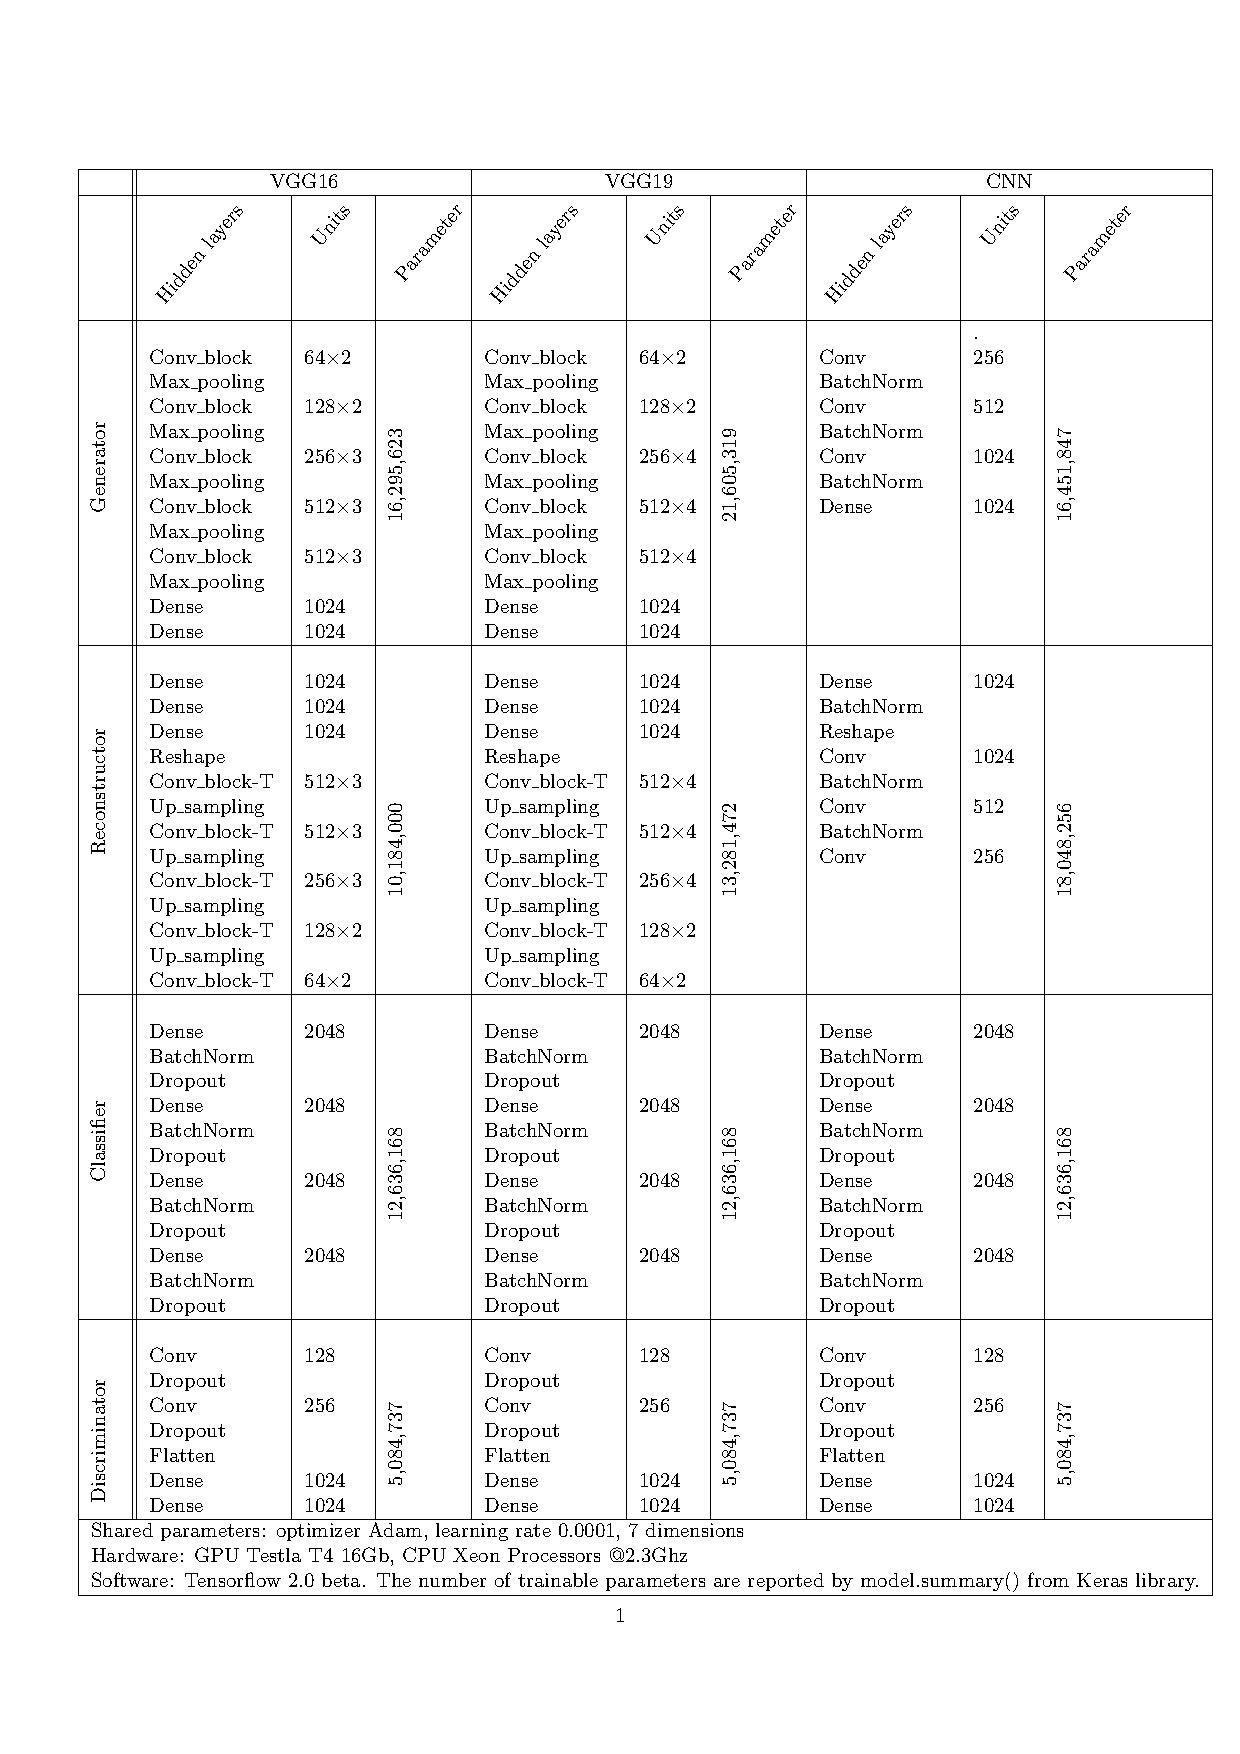
\includegraphics[width=0.9\linewidth, trim=1cm 2.5cm 0.1cm 2.5cm, clip=true]{\ChapterPathAutoGAN/tables/implement_table}
	\caption{Implementation information}
	\label{table:implementation}
\end{table*}



\begin{figure*}[ht!]
	\begin{subfigure}{.32\textwidth}
		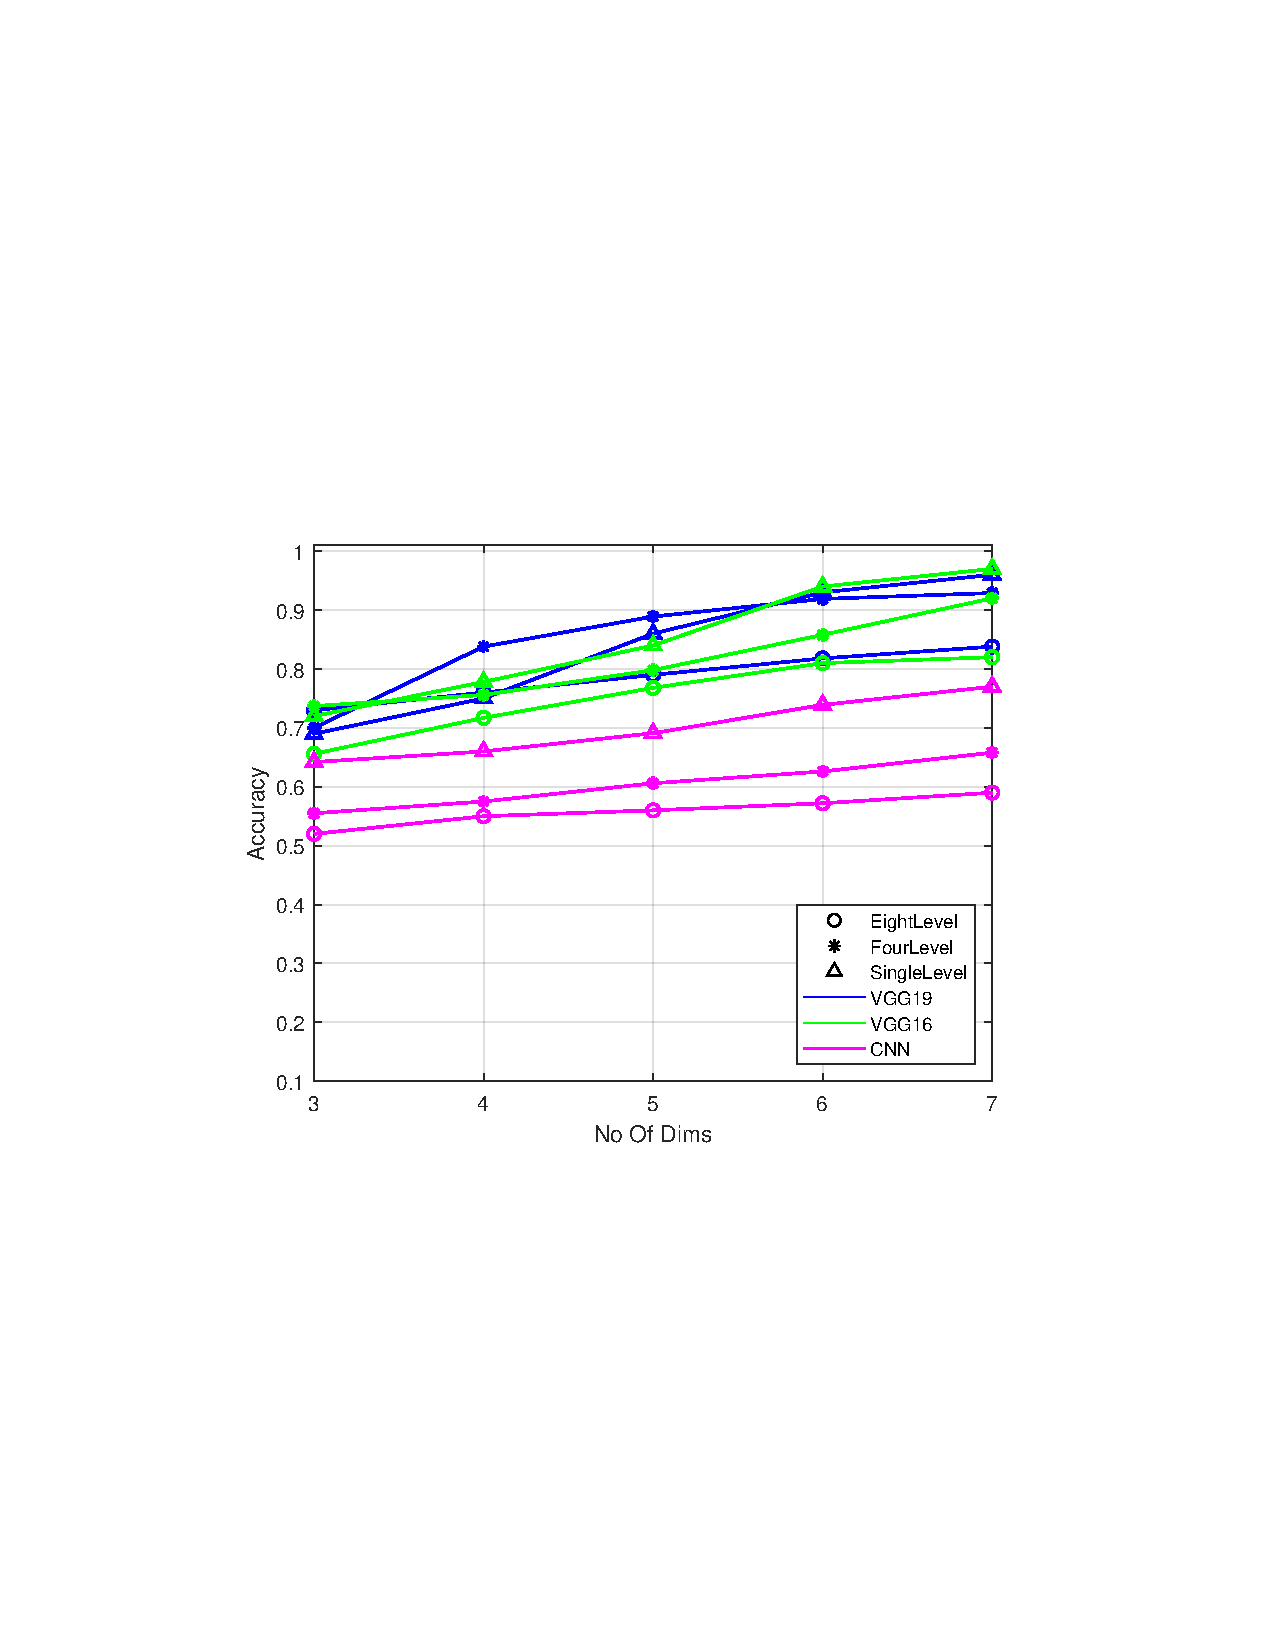
\includegraphics[width=\linewidth, trim=3.8cm 8cm 4cm 8cm, clip=true]{\ChapterPathAutoGAN/figures/att_acc}
		\captionsetup{justification=centering}
		\caption{ AT\&T}
		\label{fig:att_acc}
	\end{subfigure}
	\begin{subfigure}{.32\textwidth}
		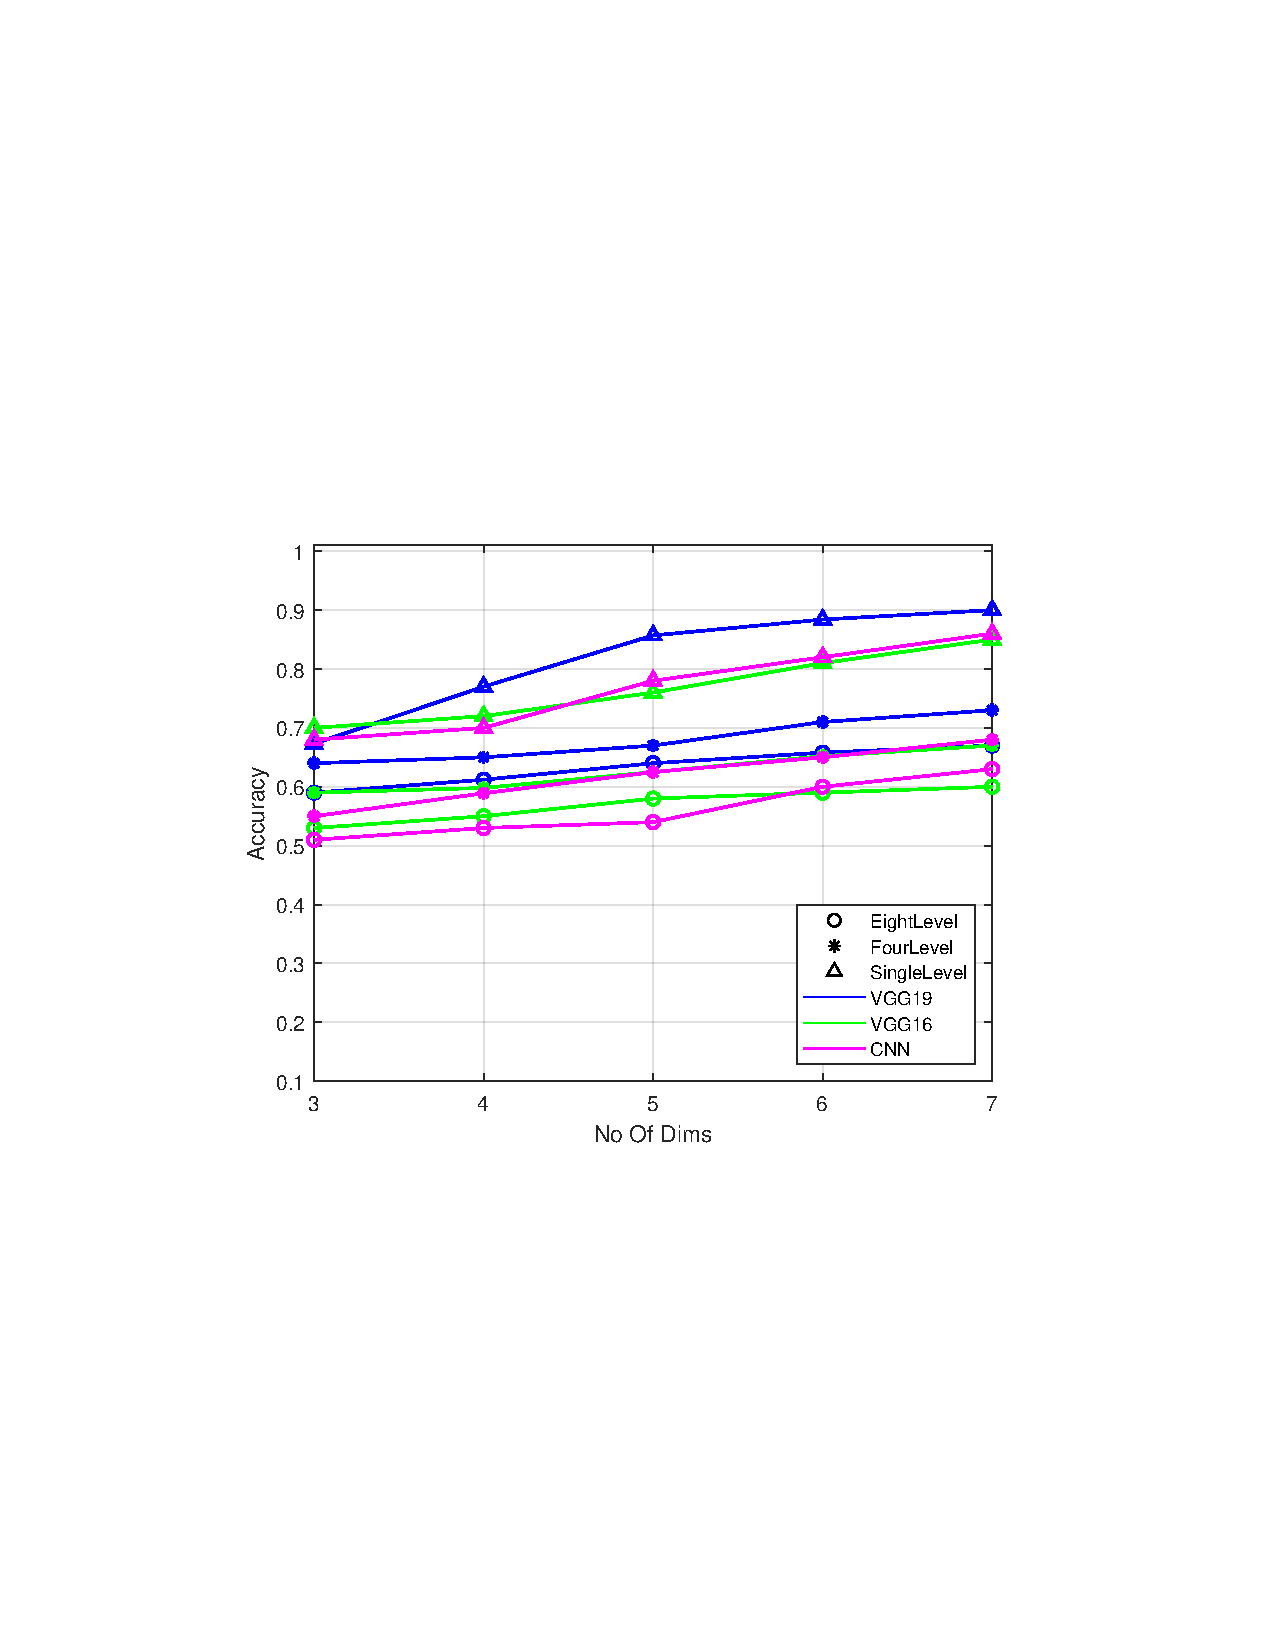
\includegraphics[width=\linewidth, trim=3.8cm 8cm 4cm 8cm, clip=true]{\ChapterPathAutoGAN/figures/yale_acc}
		\captionsetup{justification=centering}
		\caption{Yale\_B}
		\label{fig:yale_acc}
	\end{subfigure}
	\begin{subfigure}{.32\textwidth}
		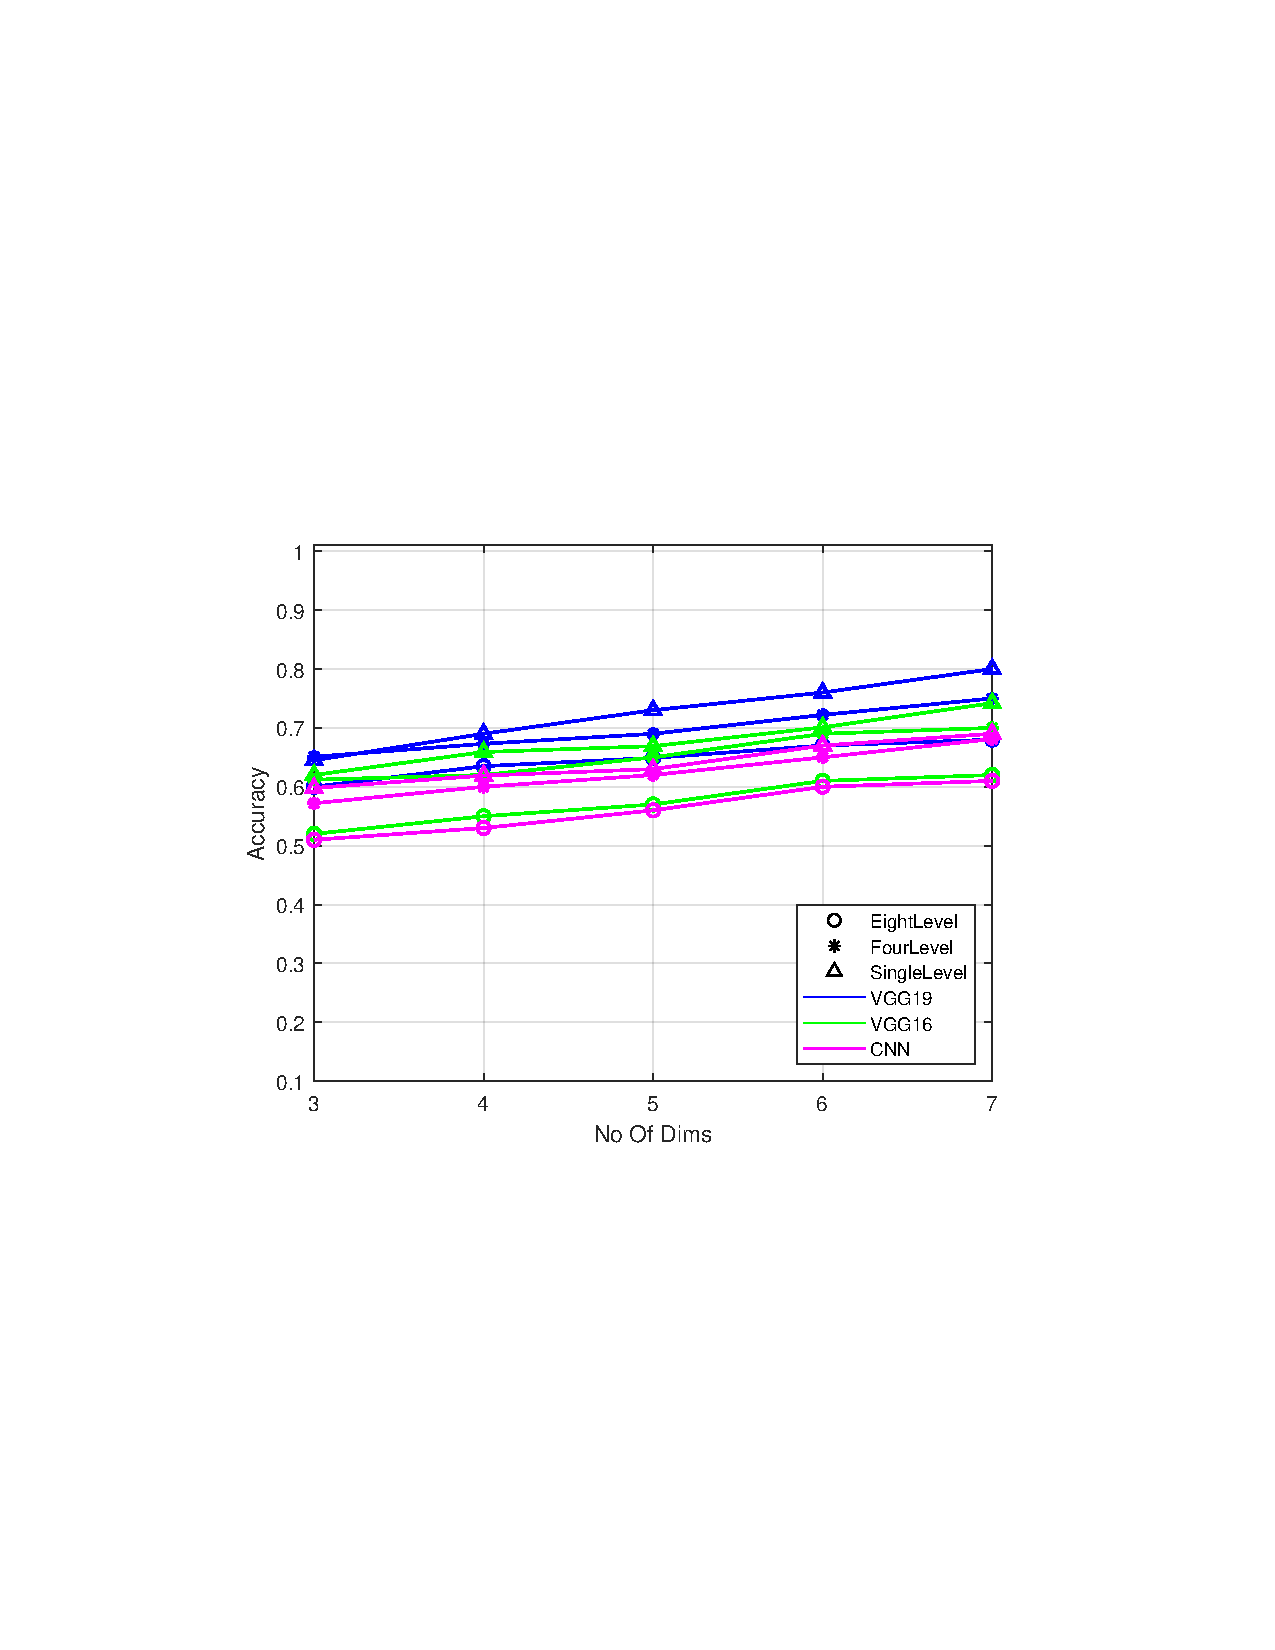
\includegraphics[width=\linewidth, trim=3.8cm 8cm 4cm 8cm, clip=true]{\ChapterPathAutoGAN/figures/celeba_acc}
		\captionsetup{justification=centering}
		\caption{CelebA}
		\label{fig:celeba_acc}
	\end{subfigure}
	\caption{Accuracy for different number of reduced dimensions. }
	\label{fig:acc}
\end{figure*}

\begin{figure*}[ht!]
	\begin{subfigure}{.32\textwidth}
		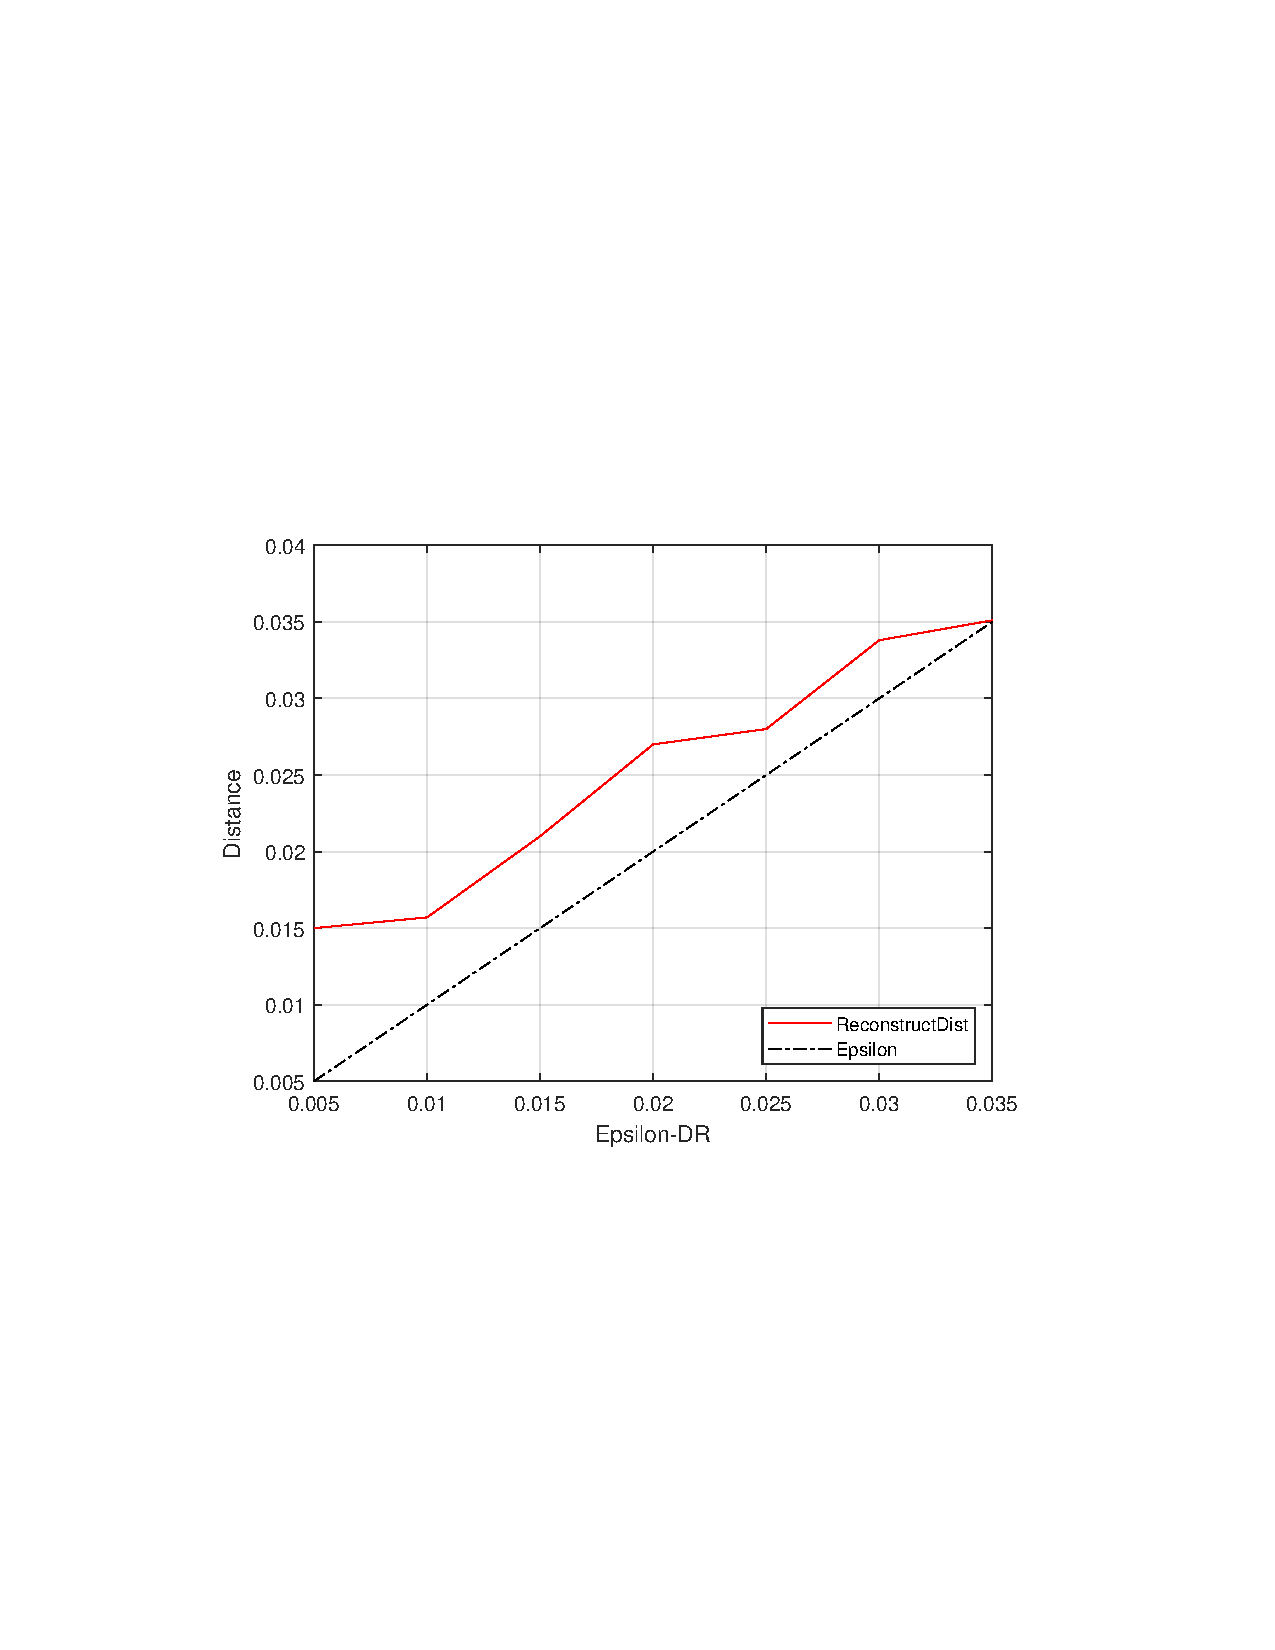
\includegraphics[width=\linewidth, trim=3.8cm 8cm 4cm 8cm, clip=true]{\ChapterPathAutoGAN/figures/ep_att}
		\captionsetup{justification=centering}
		\caption{ AT\&T}
		\label{fig:att_dist}
	\end{subfigure}
	\begin{subfigure}{.32\textwidth}
		\includegraphics[width=\linewidth, trim=3.8cm 8cm 4cm 8cm, clip=true]{\ChapterPathAutoGAN/figures/ep_yale}
		\captionsetup{justification=centering}
		\caption{Yale\_B}
		\label{fig:yale_dist}
	\end{subfigure}
	\begin{subfigure}{.32\textwidth}
		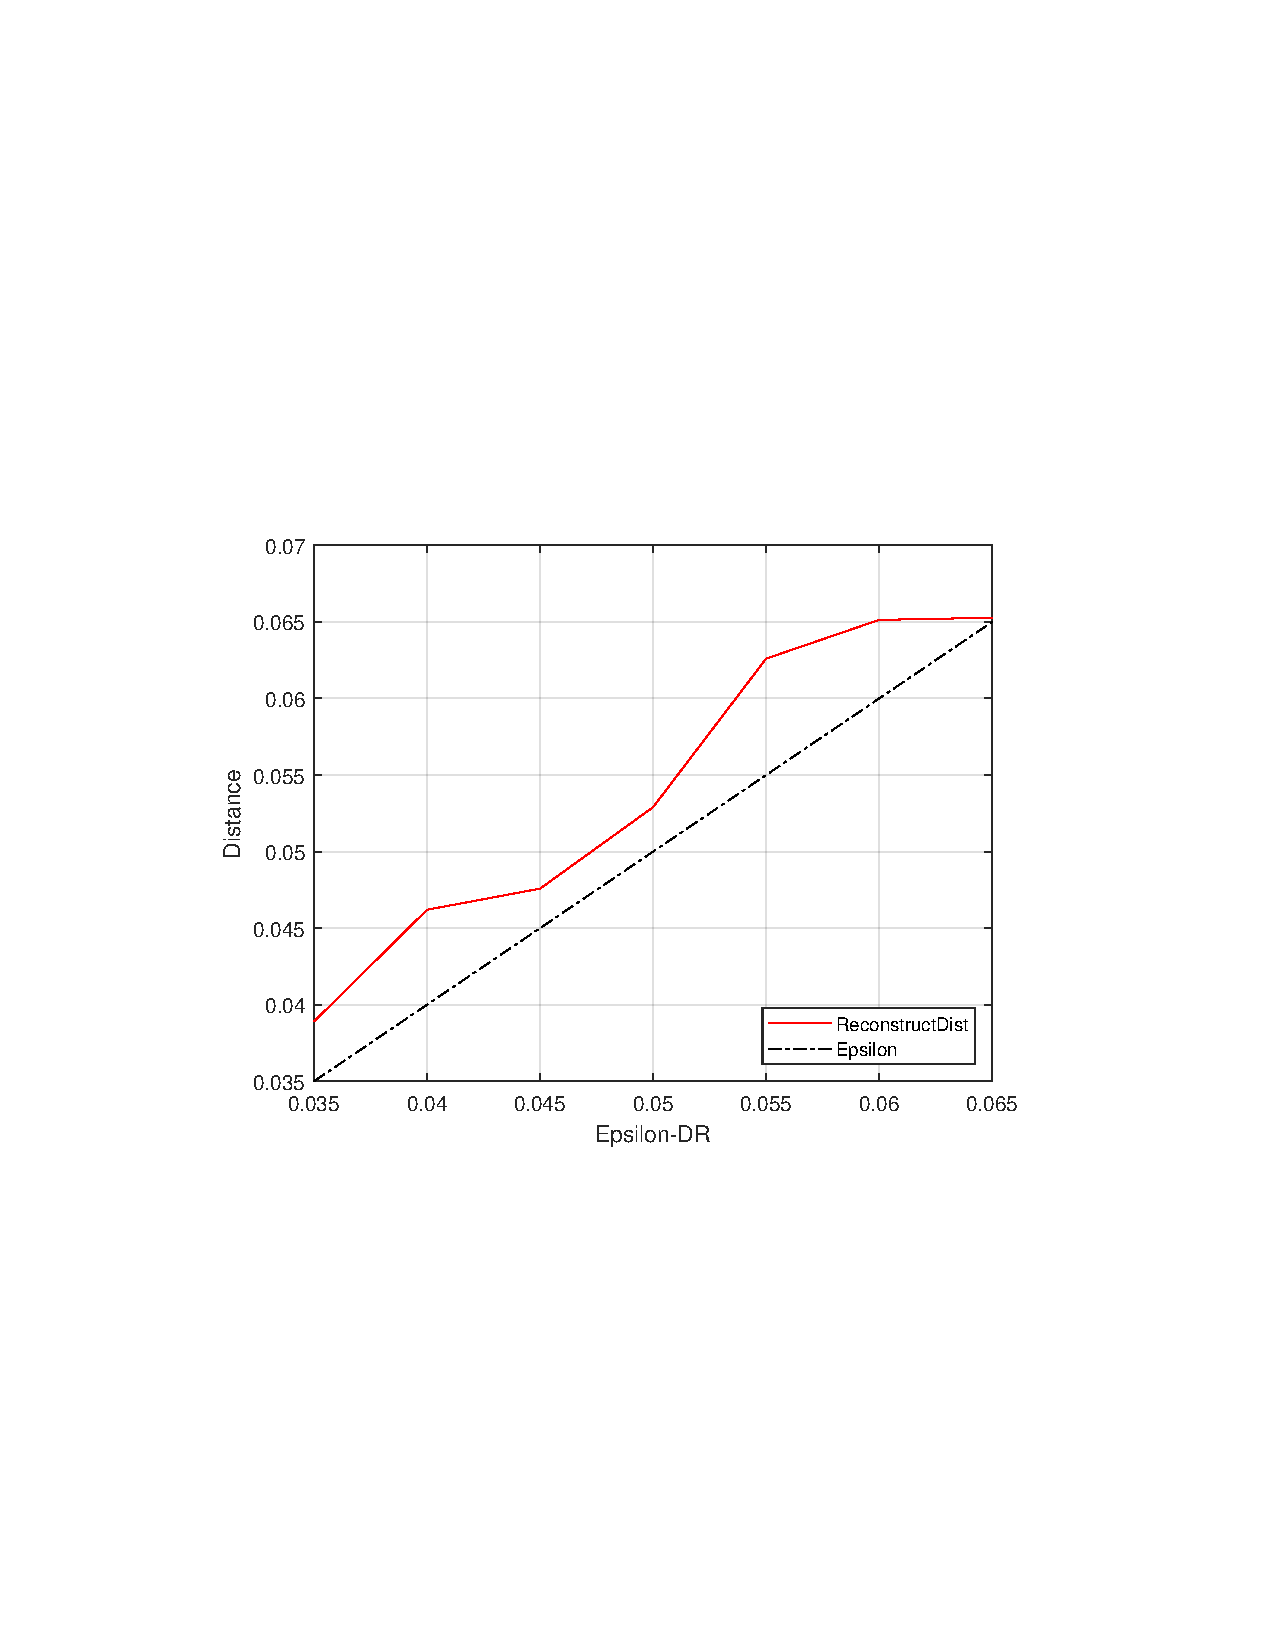
\includegraphics[width=\linewidth, trim=3.8cm 8cm 4cm 8cm, clip=true]{\ChapterPathAutoGAN/figures/ep_celeba}
		\captionsetup{justification=centering}
		\caption{CelebA}
		\label{fig:celeba_dist}
	\end{subfigure}
	\caption{Average distance measurement result.}
	\label{fig:distresult}
\end{figure*}


In this section, we demonstrate our experiments over three popular supervised face image datasets: \textit{the Extended Yale Face Database B} \cite{GeBeKr01}, \textit{AT}\&\textit{T} \cite{341300}, and \textit{CelebFaces Attributes Dataset (CelebA)} \cite{celeba}. To comprehensively evaluate our method performance, we also conduct experiments with different generator and re-constructor structures, different types of classifications (binary and multi-class classification), different numbers of reduced dimensions. The effectiveness of the method is then evaluated in terms of utility and privacy.   
\subsection{Experiment Setup}
\textit{The Extended Yale Face Database B} (YaleB) contains 2,470 grayscale images of 38 human subjects under different illumination conditions and their identity label. In this dataset, the image size is 168$\times$192 pixels. The AT\&T dataset has 400 face images of 40 subjects. For convenience, we resize each image of these two dataset to 64$\times$64 pixels. CelebA is a color facial image dataset containing 202,599 images of 10,177 subjects. 1,709 images of the first 80 subjects are used for our experiment. Each image is resized to 64$\times$64$\times$3 pixels. All pixel values are scaled to the range of [0,1]. We randomly select 10\% of each subject's images for validation and 15\% for testing dataset. 

The generator and re-constructor in Figure \ref{fig:eGAN} are implemented by three different structures. Specifically, we follow the architecture of recent powerful models VGG19, VGG16 \cite{vgg} and a basic convolutional network (CNN). We modify the models to adapt to our data size (64$\times$64). Discriminator and Classifier are built on fully connected neural network and convolutional network respectively. Leaky ReLU is used for activation function in hidden layers. We use linear activation function for generator's output layers and softmax activation functions for other components' output layers. Each component is trained in 5 local iterations ($n_r, n_g, n_d, n_c$), and the entire system is trained in 500 global iterations ($n$). The target distribution is drawn from Gaussian distribution (with the covariance value of 0.5 and the mean is the average of the training data). Table \ref{table:implementation} provides detail information of neural networks' structures and other implementation information. 
 
To evaluate the reliability, we test our framework with different levels of authentication corresponding to binary classification (single-level) and multi-class classification (multi-level). For the single-level authentication system, we consider half of the subjects in the dataset are valid to access company's resources while the rest are invalid. We randomly divide the dataset into two groups of subjects and labels their images to (1) or (0) depending on their access permission. For the cases of multi-level authentication system, we divide the subjects into four groups and eight groups. Therefore, the authentication server becomes four-class and eight-class classifier respectively. 
\subsection{Utility}
We use accuracy metric to evaluate the utility of dimension-reduced data. The testing dataset is tested with the classifier extracted from our framework. Different structures of Generator and re-constructor are applied including VGG19, VGG16, basic CNN on different privilege levels which correspond to multi-class classification. Figure \ref{fig:acc} illustrates the accuracies for different dimensions from three to seven over the three facial datasets. Overall, the accuracies improve when the number of dimension increases. The accuracies on the two gray image datasets (AT\&T and Yale\_B) reaches 90\% and higher when using VGG with only seven dimensions. This accuracy figure for Celeba is smaller, but it still reaches 80\%. In general, VGG19 structure performs better than using VGG16 and basic CNN in terms of utility due to the complexity (table \ref{table:implementation}) and adaptability to image datasets of VGG19. As the dimension number is reduced from 4,096 (64$\times$64) to 7, we can achieve a compression ratio of 585 yet achieve accuracy of 90\% for the two gray datasets and 80\% for the color dataset. This implies our method could gain a high compression ratio and maintain a high utility in terms of accuracy. During conducting experiments we also observe that the accuracy could be higher if we keep the original resolution of images. However, for convenience and reducing the complexity of our structure, we resize images to the size of 64$\times$64 pixels.    

\subsection{Privacy}
In this study, the Euclidean distance is used to measure the distance between original and reconstructed images: $dist(x,\hat{x}) = ||x-\hat{x}||^2$. Figure \ref{fig:distresult} illustrates the average distances between original images and reconstructed images on testing data with different $\epsilon$ constraints (other setting parameters: seven dimensions, single-level authentication, and VGG19 structure). The achieved distances (red lines) are larger than the hyper-parameter $\epsilon$ (black dotted lines) where $\epsilon$ is less than 0.035 for AT\&T, 0.052 for YaleB and 0.067 for CelebA. Thus, our framework can satisfy $\epsilon$-DR with $\epsilon$ of above values. Due to the fact that the re-constructor obtained some information (we consider the adversary can reach the model and the training data), we can only set the distance constraint $\epsilon$ within a certain range as shown in \ref{fig:distresult}. The intersection between the red line and the dotted black line points out the largest distance our framework can achieve. Since the mean of the target distribution is set to be the same as the mean of training dataset, reconstructed images will be close to the mean of training dataset which we believe it will enlarge the distance and expose less individual information. Thus, the range of epsilon can be estimated base on the expectation of the distance between testing samples and the mean of training data. In addition, the first section of Table \ref{table:visualization} demonstrates some samples and their corresponding reconstructions in single-level authentication and seven dimensions with different achieved accuracies and distances. The reconstructed images could be nearly identical, thus making it visually difficult to recognize the identity of an individual.      

\section{Comparison to GAP\cite{GAP}}
\label{sec:AutoGAN_GAP}

In this section, we compare the proposed framework with GAP, which shares many similarities. At first, we attempt to visualize AutoGAN-DRP and GAP by highlighting their similarities and differences. Then, we exhibit our experiment results of the two methods on the same dataset. 

In terms of similarities, AutoGAN-DRP and GAP are utilizing minimax algorithms of Generative Adversarial Nets, applying the state-of-the-art convolution neural nets for image datasets, considering $l_2$ norm distance (i.e., distortion in GAP, privacy measurement in AutoGAN-DRP) between the original images and reconstructed images. Specifically, both GAP and AutoGAN-DRP consider the reconstruction distance between original and reconstructed images. In GAP this \textit{distortion} refers to the Euclidean between original and privatized images, and AutoGAN-DRP denotes the \textit{distance} as the Euclidean distance between original and reconstructed images. In this context, the distance and distortion refer to the same measurement and have the same meaning. To be consistent, we use the term \textit{distance} to present this measurement in the rest of this section.

However, there are also distinctions between GAP and AutoGAN-DRP. In GAP, the adversary aims to identify a private label (e.g., gender) which should be kept secret while AutoGAN-DRP aims to visually protect the owner's face images by enlarging the reconstruction distance. Thus, instead of considering a private label in loss function of the generator in GAP, AutoGAN-DRP is aimed at driving the reconstructed data into a target distribution using a discriminator.   
   
\begin{figure}
	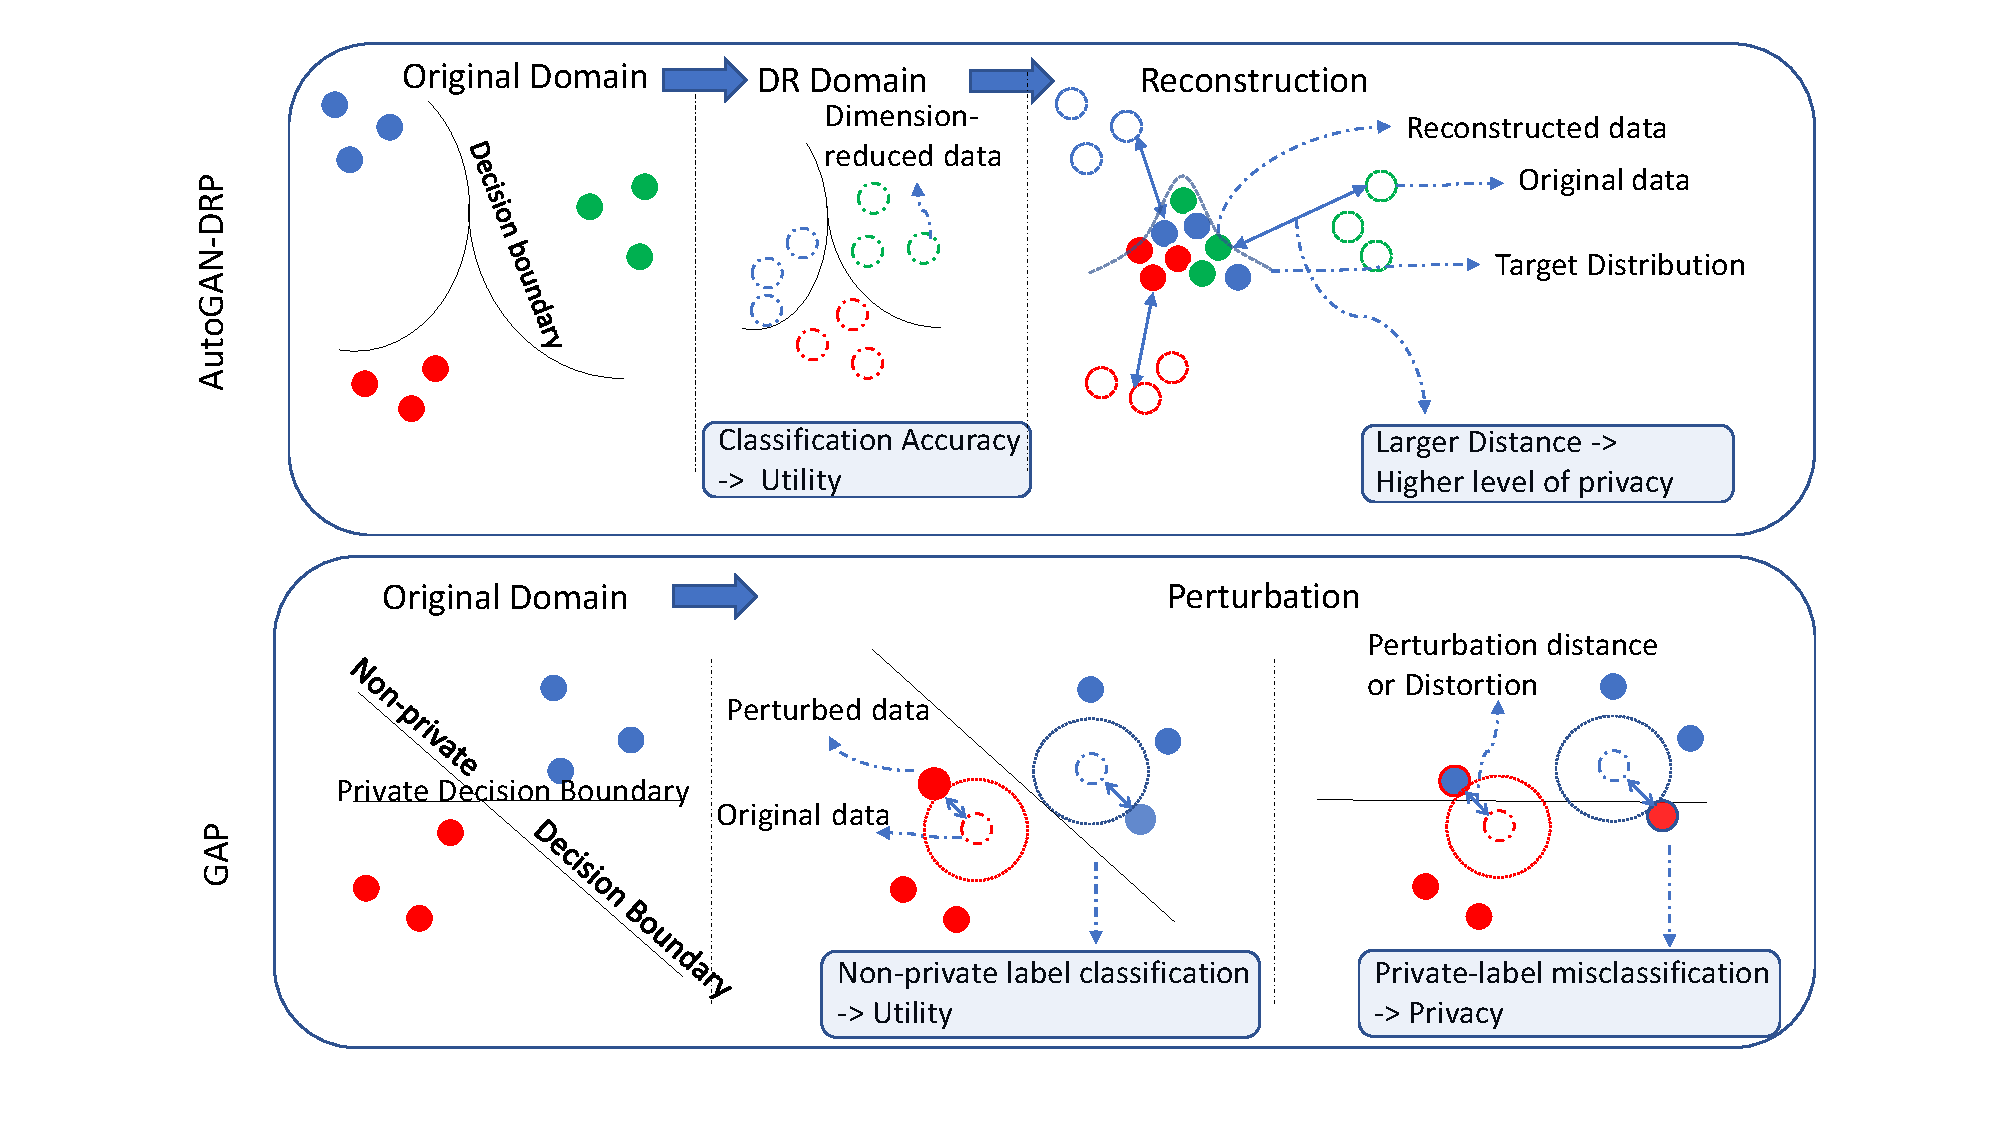
\includegraphics[width=\linewidth,trim=2.7cm 0.5cm 2.5cm 0.5cm, clip=true]{\ChapterPathAutoGAN/figures/GAPvsAGDRPP}
	\caption{AutoGAN-DRP and GAP visualization.}
	\label{fig:AGDRPPvsGAP}
\end{figure}
      
Figure \ref{fig:AGDRPPvsGAP} illustrates the visualization of AutoGAN-DRP and GAP. In AutoGAN-DRP, privacy is assessed based on how well an adversary can reconstruct the original data and measured by the distance between original and reconstructed data. The dimension-reduced data is reconstructed using the state-of-the-art neural network (an Auto-encoder). The larger the distance is, the more privacy can be achieved. Further, if the reconstructed images are blurry, privacy can be preserved since it is hard to visually determine an individual identity. The data utility is quantified by the accuracy of the classification tasks over dimension-reduced data which captures the most significant data information. Meanwhile, GAP perturbs images with a certain distortion constraint to achieve privacy. It evaluates data utility by the classification accuracy of non-private label and assesses privacy by the classification accuracy of private label. Similar to AutoGAN-DRP, the high distortion is most likely to yield high level of privacy. In GAP, however, high distortion might dramatically reduce the classification accuracy of non-private label. This might be caused by the high correlation between private and non-private labels. This difference enables AutoGAN-DRP to preserve more utility than GAP at the same distortion level, as the experiment result (depicted in Figure \ref{fig:genki}) reveals. 

\begin{figure}[H]
	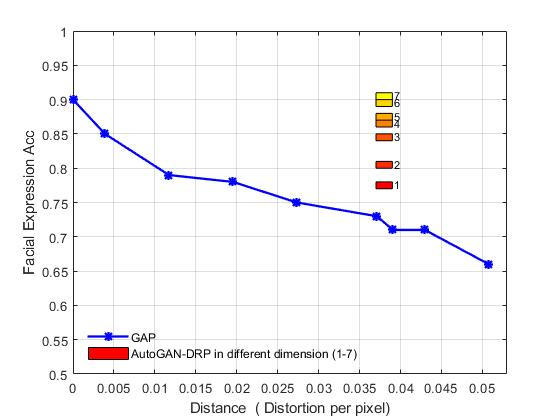
\includegraphics[width=\linewidth]{\ChapterPathAutoGAN/figures/ACC_AutoGANvsGAP}
	\caption[Facial expression accuracy and distance.]{GENKI Facial Expression Accuracy Vs Distance using GAP and AutoGAN-DRP}
	\label{fig:genki}
\end{figure}

In the experiment, we reproduce a prototype of Transposed Convolutional Neural Nets Privatizer (TCNNP) in GAP using materials and source code provided by \cite{GAP}. We also modify our framework to make it as similar to TCNNP as possible. Specifically, a combination of two convolutional layers with ReLU activation function and two fully connected neural network layers are used for implementing the Generator similar to TCNNP. Our Classifier is constructed on two convolutional layers and two fully connected hidden layers similar to the Adversary in GAP. We also test our framework on GENKI, the same dataset with GAP. The utility is evaluated by the accuracy of facial expression classification (a binary classification). It should be noted that our framework have been shown to work on different datasets with multi-class classification, which is more challenging and comprehensive. Figure \ref{fig:genki} shows the accuracy results of GAP and AutoGAN-DRP for GENKI dataset. AutoGAN-DRP achieves distances ranging from 0.037 to 0.039 for different dimensions from one to seven. At the same range of distance (distortion per pixel), GAP achieves accuracy of only 72\% while AutoGAN-DRP gains accuracy rates starting from 77\% to 91\% for different number of dimensions. It becomes evident that our method can achieve higher accuracy than that of GAP at the same distortion level.        



\section{Visual Comparison to Privacy Preserving Techniques}
\label{sec:AutoGAN_DP_PCA}

In this section, we compare AutoGAN-DRP with other privacy preserving methods in terms of ability to visually identify client's identities. We choose the widely used tool for privacy preserving Differential Privacy (DP) \cite{Dwork2006} and another privacy preservation method utilizing dimensionality reduction technique (i.e., Principle Component Analysis \cite{PCA} ).
 
 \begin{table*}[http!]
 	\centering
 	%trim  left, bottom, right and top 
 	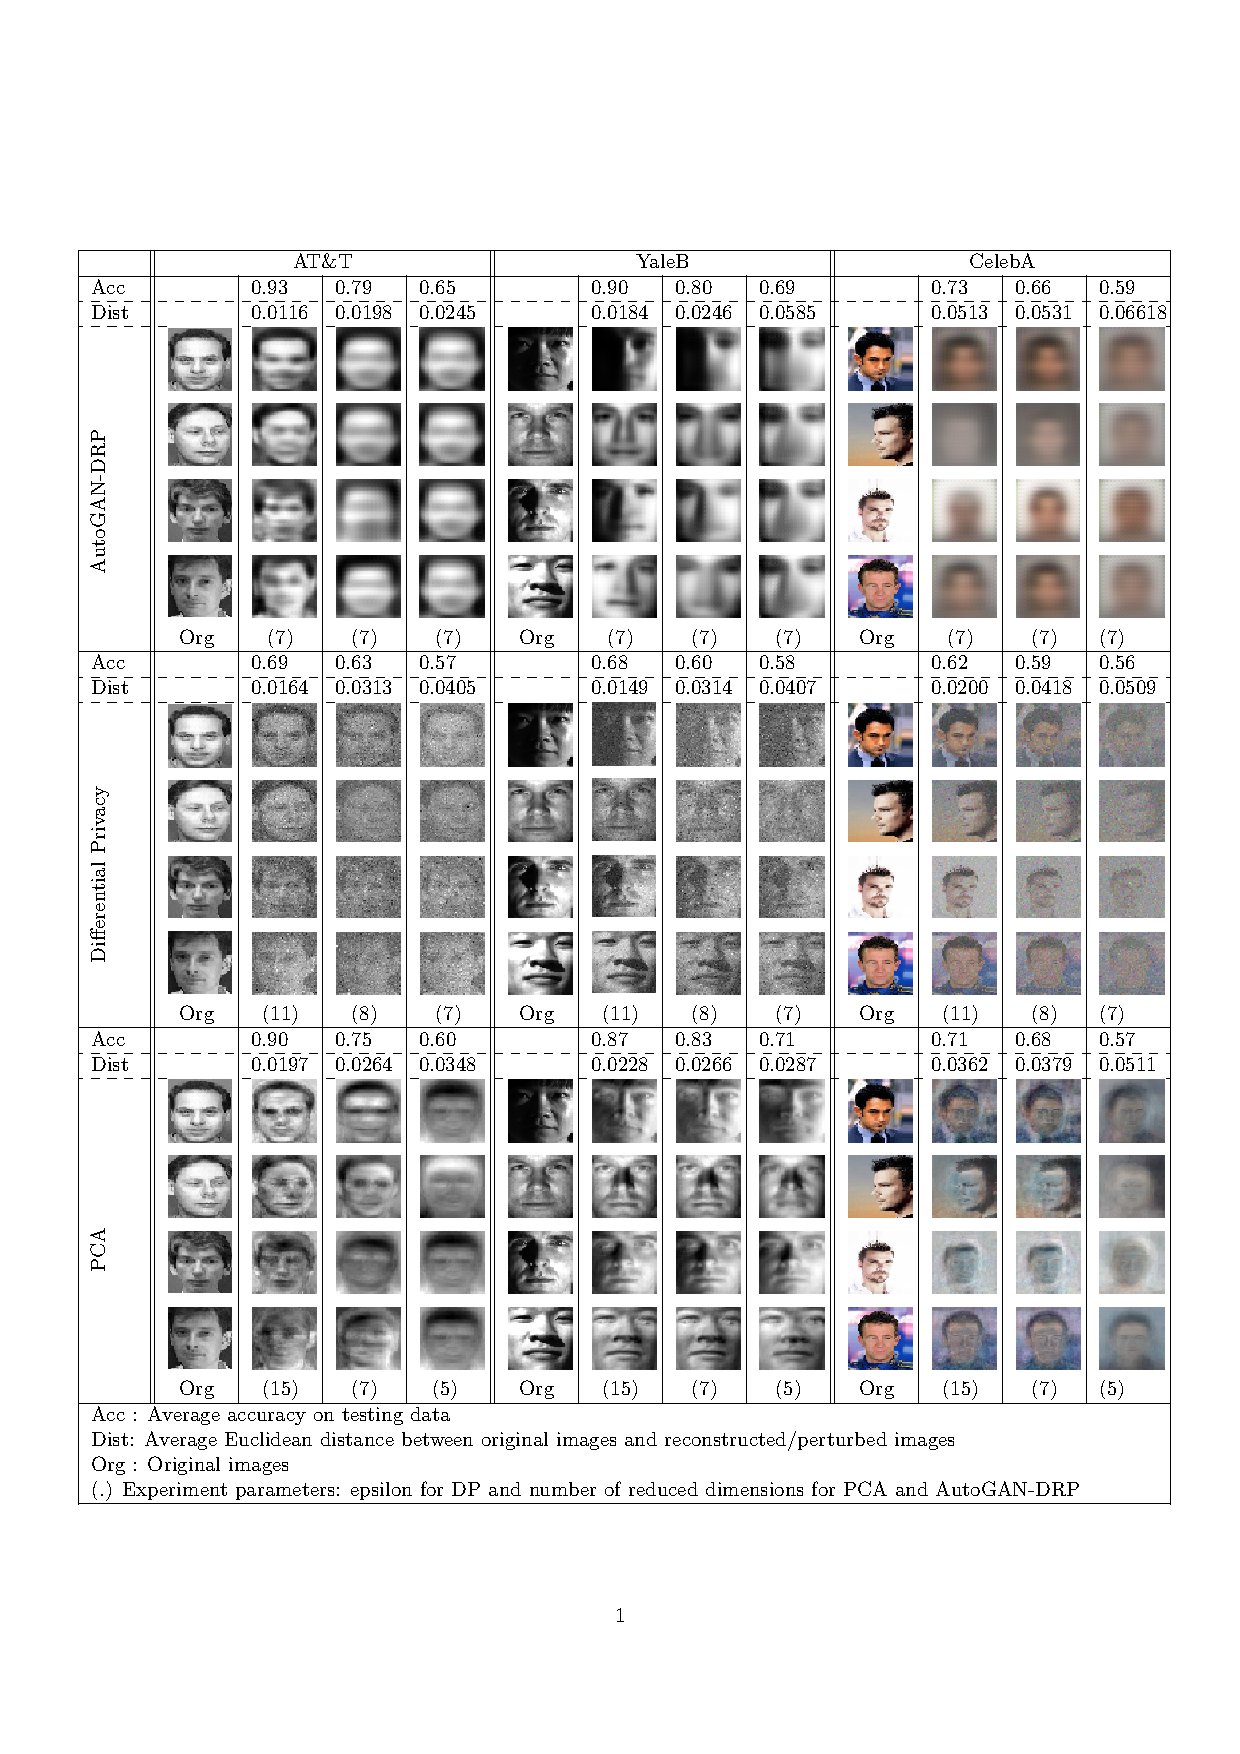
\includegraphics[width=0.9\linewidth, trim=1cm 3cm 1cm 3cm, clip=true]{\ChapterPathAutoGAN/tables/img_table}
 	\caption{Sample visualization of AutoGAN, DP, PCA over three datasets}
 	\label{table:visualization}
 \end{table*}
 
In these experiments, we implement AutoGAN-DRP following VGG19 structure for the Generator and Re-constructor, and other setting parameters (e.g., number of hidden layers, learning rate, optimization) are shown in Table \ref{table:implementation}. The images are reduced to seven dimensions for different values of $\epsilon$-DR to achieve different distances and accuracies. The datasets are grouped into two groups corresponding to a binary classifier. 

For implementing DP, we first generate a classifier on the authentication server by training the datasets with a VGG19 binary classifier (the structure of hidden layers is similar to our Generator in Table \ref{table:implementation}). The testing images are then perturbed using differential privacy method. Specifically, Laplace noise is added to the images with the sensitivity coefficient of 1 (it is computed by the maximum range value of each pixel [0,1]) and different DP epsilon parameters (this DP epsilon is different from our $\epsilon$-DR). The perturbed images are then sent to the authentication server and fed to the classifier. We visually compare the perturbed images of this method with AutoGAN. 

In addition, we follow instruction in FRiPAL \cite{zhuang2017fripal} in which the clients reduce image dimension using Principle Component Analysis (PCA) and send reduced features to the server. FRiPAL claims that by reducing image dimension, their method can be more resilient to reconstruction attacks. The experiments are conducted with different number of reduced dimension. The images are reconstructed using \textit{Moore–Penrose inverse} method with assumption that an adversary has assess to the model. The classification accuracy is evaluated using a classifier which has similar structure to AutoGAN's classifier. 

Table \ref{table:visualization} shows image samples and results over the three datasets. Overall, AutoGAN-DRP is more resilient to reconstruction attacks compared to the other two techniques. For instance, at the accuracy of 79\% on AT\&T dataset, 80\% on YaleB, and 73\% on CelebA, we cannot distinguish entities from the others. For DP method, the accuracy decreases when the DP epsilon decreases (adding more noise), and the perturbed images become harder to recognize. However, at a low accuracy 57\%, we are still able to distinguish identities by human eyes. The reason is that DP noise does not focus on the important visual pixels. For PCA, the accuracy also goes down when the number of dimensions decreases and the distances increase. Since PCA transformation is linear and deterministic, the original information can be significantly reconstructed using the inverse transformation deriving from the model or training data. Thus, at the accuracy of 75\% on AT\&T, 71\% on YaleB, and 68\% on CelebA, we still can differentiate individuals. Overall, our proposed method shows the advantage in securing the data while retaining high data utility.       




\section{Conclusion}
\label{sec:Autogan_conclusion}
In this work, we introduce a mathematical tool $\epsilon$-DR to evaluate privacy preserving mechanisms. We also propose a non-linear dimension reduction framework. This framework projects data onto lower dimension domain in which it prevents reconstruction attacks and preserves data utility. The dimension-reduced data can be used effectively for the machine learning tasks such as classification. In our future works, we plan to extend the framework to adapt with different types of data, such as time series and categorical data. We will apply different metrics to compute the distance other than $l_2$ norm and investigate the framework on several applications in security systems and data collaborative contributed systems.  









\begin{spacing}{1}
\bibliographystyle{plain}
\interlinepenalty=10000
\bibliography{template}
\end{spacing}


\begin{appendices}

\chapter{Copyright Permissions}\label{cp:apex}
The permission below is for the reproduction of material in Chapter \ref{chap:AUTOGAN}.
\begin{figure}[!ht]
	\centering
    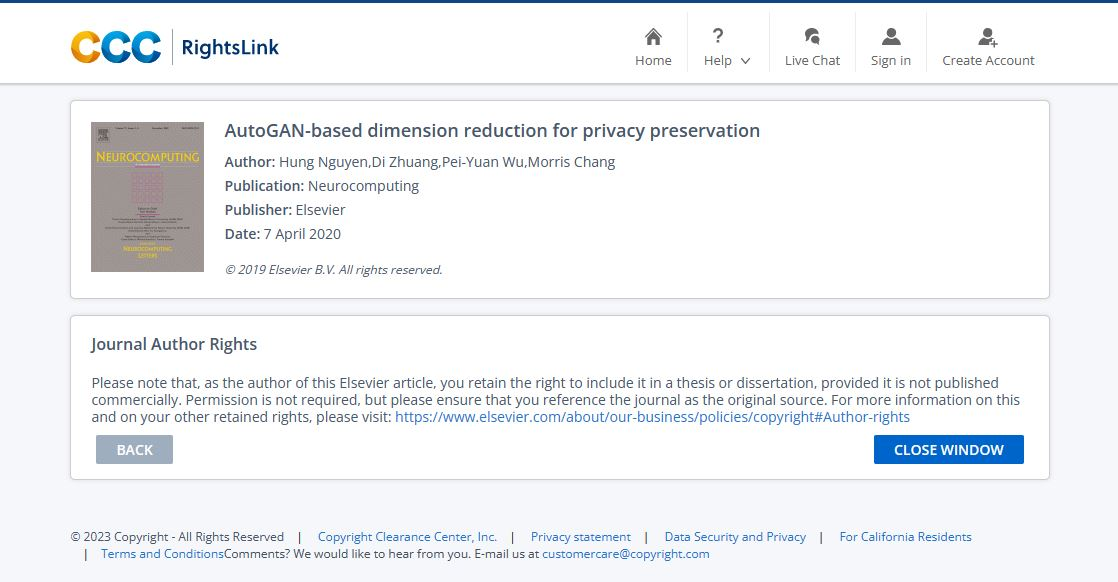
\includegraphics[width=0.9\textwidth]{Figures/copyright}
	\label{copyright1}
\end{figure} 


\end{appendices}


%\printvita



\end{document}

